%% abtex2-modelo-trabalho-academico.tex, v<VERSION> laurocesar
%% Copyright 2012-<COPYRIGHT_YEAR> by abnTeX2 group at http://www.abntex.net.br/ 
%%
%% This work may be distributed and/or modified under the
%% conditions of the LaTeX Project Public License, either version 1.3
%% of this license or (at your option) any later version.
%% The latest version of this license is in
%%   http://www.latex-project.org/lppl.txt
%% and version 1.3 or later is part of all distributions of LaTeX
%% version 2005/12/01 or later.
%%
%% This work has the LPPL maintenance status `maintained'.
%% 
%% The Current Maintainer of this work is the abnTeX2 team, led
%% by Lauro César Araujo. Further information are available on 
%% http://www.abntex.net.br/
%%
%% This work consists of the files abntex2-modelo-trabalho-academico.tex,
%% abntex2-modelo-include-comandos and abntex2-modelo-references.bib
%%

% ------------------------------------------------------------------------
% ------------------------------------------------------------------------
% abnTeX2: Modelo de Trabalho Academico (tese de doutorado, dissertacao de
% mestrado e trabalhos monograficos em geral) em conformidade com 
% ABNT NBR 14724:2011: Informacao e documentacao - Trabalhos academicos -
% Apresentacao
% ------------------------------------------------------------------------
% ------------------------------------------------------------------------

\documentclass[
	% -- opções da classe memoir --
	12pt,				% tamanho da fonte
	openany,			% capítulos começam em pág ímpar (insere página vazia caso preciso)
	twoside,			% para impressão em recto e verso. Oposto a oneside
	a4paper,			% tamanho do papel. 
	% -- opções da classe abntex2 --
	chapter=TITLE,		% títulos de capítulos convertidos em letras maiúsculas
	section=Title,		% títulos de seções convertidos em letras maiúsculas
	subsection=Title,	% títulos de subseções convertidos em letras maiúsculas
	subsubsection=Title,% títulos de subsubseções convertidos em letras maiúsculas
	% -- opções do pacote babel --
	english,			% idioma adicional para hifenização
	french,				% idioma adicional para hifenização
	spanish,			% idioma adicional para hifenização
	brazil			% o último idioma é o principal do documento
	]{abntex2}



% ---
% Pacotes básicos 
% ---
\usepackage[boxruled,linesnumbered,portuguese]{algorithm2e}
% \usepackage{float}
% \usepackage{algorithm}
% \usepackage{algpseudocode}

\usepackage{tablefootnote}
\usepackage{makecell}
\usepackage{amsmath}
\usepackage{amsfonts} % for "\mathbb" macro
\newcommand{\N}{\mathbb{N}}
\newcommand{\Z}{\mathbb{Z}}
\newcommand{\Q}{\mathbb{Q}}
\newcommand{\R}{\mathbb{R}}
\newcommand{\C}{\mathbb{C}}
\usepackage{lmodern}			% Usa a fonte Latin Modern
\usepackage{longtable}
\usepackage[T1]{fontenc}		% Selecao de codigos de fonte.
\usepackage[utf8]{inputenc}		% Codificacao do documento (conversão automática dos acentos)
\usepackage{indentfirst}		% Indenta o primeiro parágrafo de cada seção.
\usepackage{color}				% Controle das cores
\usepackage{graphicx}			% Inclusão de gráficos
\usepackage{microtype} 			% para melhorias de justificação
% ---
		
% ---
% Pacotes adicionais, usados apenas no âmbito do Modelo Canônico do abnteX2
% ---
\usepackage{lipsum}				% para geração de dummy text
% ---

% ---
% Pacotes de citações
% ---
\usepackage[brazilian,hyperpageref]{backref}	 % Paginas com as citações na bibl
\usepackage[alf]{abntex2cite}	% Citações padrão ABNT
\renewcommand{\ABNTEXchapterfont}{\fontfamily{lmr}\fontseries{b}\selectfont}
% --- 
% CONFIGURAÇÕES DE PACOTES
% --- 

% ---
% Configurações do pacote backref
% Usado sem a opção hyperpageref de backref
\renewcommand{\backrefpagesname}{Citado na(s) página(s):~}
% Texto padrão antes do número das páginas
\renewcommand{\backref}{}
% Define os textos da citação
\renewcommand*{\backrefalt}[4]{
	\ifcase #1 %
		Nenhuma citação no texto.%
	\or
		Citado na página #2.%
	\else
		Citado #1 vezes nas páginas #2.%
	\fi}%
% ---

% ---
% Informações de dados para CAPA e FOLHA DE ROSTO
% ---
\setcounter{page}{1}
\titulo{Método híbrido de Enxame de Partículas de Aprendizagem Abrangente com Programação Quadrática Sequencial e \emph{Branch-and-Bound} para resolução de problemas do Fluxo de Potência Ótimo com variáveis discretas.}
\autor{Equipe \abnTeX}
\local{Brasil}
\data{2018, v<VERSION>}
\orientador{Lauro César Araujo}
\coorientador{Equipe \abnTeX}
\instituicao{%
  Universidade do Brasil -- UBr
  \par
  Faculdade de Arquitetura da Informação
  \par
  Programa de Pós-Graduação}
\tipotrabalho{Tese (Doutorado)}
% O preambulo deve conter o tipo do trabalho, o objetivo, 
% o nome da instituição e a área de concentração 
\preambulo{Método Híbrido de Enxame de Partículas de Aprendizagem Abrangente com Programação Sequencial Quadrática e \emph{Branch-and-Bound}.}
% ---


% ---
% Configurações de aparência do PDF final

% alterando o aspecto da cor azul
\definecolor{blue}{RGB}{41,5,195}

% informações do PDF
\makeatletter
\hypersetup{
     	%pagebackref=true,
		pdftitle={\@title}, 
		pdfauthor={\@author},
    	pdfsubject={\imprimirpreambulo},
	    pdfcreator={LaTeX with abnTeX2},
		pdfkeywords={abnt}{latex}{abntex}{abntex2}{trabalho acadêmico}, 
		colorlinks=true,       		% false: boxed links; true: colored links
    	linkcolor=blue,          	% color of internal links
    	citecolor=blue,        		% color of links to bibliography
    	filecolor=magenta,      		% color of file links
		urlcolor=blue,
		bookmarksdepth=4
}
\makeatother
% --- 

% ---
% Posiciona figuras e tabelas no topo da página quando adicionadas sozinhas
% em um página em branco. Ver https://github.com/abntex/abntex2/issues/170
\makeatletter
\setlength{\@fptop}{5pt} % Set distance from top of page to first float
\makeatother
% ---

% ---% ---
% Possibilita criação de Quadros e Lista de quadros.
% Ver https://github.com/abntex/abntex2/issues/176
%
\newcommand{\quadroname}{Quadro}
\newcommand{\listofquadrosname}{Lista de quadros}

\newfloat[chapter]{quadro}{loq}{\quadroname}
\newlistof{listofquadros}{loq}{\listofquadrosname}
\newlistentry{quadro}{loq}{0}

% configurações para atender às regras da ABNT
\setfloatadjustment{quadro}{\centering}
\counterwithout{quadro}{chapter}
\renewcommand{\cftquadroname}{\quadroname\space} 
\renewcommand*{\cftquadroaftersnum}{\hfill--\hfill}

\setfloatlocations{quadro}{hbtp} % Ver https://github.com/abntex/abntex2/issues/176
% ---

% --- 
% Espaçamentos entre linhas e parágrafos 
% --- 

% O tamanho do parágrafo é dado por:
\setlength{\parindent}{1.3cm}

% Controle do espaçamento entre um parágrafo e outro:
\setlength{\parskip}{0.2cm}  % tente também \onelineskip

% ---
% compila o indice
% ---
\makeindex
% ---

% ----
% Início do documento
% ----
\begin{document}

% Seleciona o idioma do documento (conforme pacotes do babel)
%\selectlanguage{english}
\selectlanguage{brazil}

% Retira espaço extra obsoleto entre as frases.
\frenchspacing 

% ----------------------------------------------------------
% ELEMENTOS PRÉ-TEXTUAIS
% ----------------------------------------------------------
% \pretextual

% ---
% Capa
% ---
\imprimircapa
% ---

% ---
% Folha de rosto
% (o * indica que haverá a ficha bibliográfica)
% ---
\imprimirfolhaderosto*
% ---

% ---
% Inserir a ficha bibliografica
% ---

% Isto é um exemplo de Ficha Catalográfica, ou ``Dados internacionais de
% catalogação-na-publicação''. Você pode utilizar este modelo como referência. 
% Porém, provavelmente a biblioteca da sua universidade lhe fornecerá um PDF
% com a ficha catalográfica definitiva após a defesa do trabalho. Quando estiver
% com o documento, salve-o como PDF no diretório do seu projeto e substitua todo
% o conteúdo de implementação deste arquivo pelo comando abaixo:
%
% \begin{fichacatalografica}
%     \includepdf{fig_ficha_catalografica.pdf}
% \end{fichacatalografica}

\begin{fichacatalografica}
	\sffamily
	\vspace*{\fill}					% Posição vertical
	\begin{center}					% Minipage Centralizado
	\fbox{\begin{minipage}[c][8cm]{13.5cm}		% Largura
	\small
	\imprimirautor
	%Sobrenome, Nome do autor
	
	\hspace{0.5cm} \imprimirtitulo  / \imprimirautor. --
	\imprimirlocal, \imprimirdata-
	
	\hspace{0.5cm} \thelastpage p. : il. (algumas color.) ; 30 cm.\\
	
	\hspace{0.5cm} \imprimirorientadorRotulo~\imprimirorientador\\
	
	\hspace{0.5cm}
	\parbox[t]{\textwidth}{\imprimirtipotrabalho~--~\imprimirinstituicao,
	\imprimirdata.}\\
	
	\hspace{0.5cm}
		1. Palavra-chave1.
		2. Palavra-chave2.
		2. Palavra-chave3.
		I. Orientador.
		II. Universidade xxx.
		III. Faculdade de xxx.
		IV. Título 			
	\end{minipage}}
	\end{center}
\end{fichacatalografica}
% ---

% ---
% Inserir errata
% ---
\begin{ERRATA}
Elemento opcional da \citeonline[4.2.1.2]{NBR14724:2011}. Exemplo:


\vspace{\onelineskip}

FERRIGNO, C. R. A. \textbf{Tratamento de neoplasias ósseas apendiculares com
reimplantação de enxerto ósseo autólogo autoclavado associado ao plasma
rico em plaquetas}: estudo crítico na cirurgia de preservação de membro em
cães. 2011. 128 f. Tese (Livre-Docência) - Faculdade de Medicina Veterinária e
Zootecnia, Universidade de São Paulo, São Paulo, 2011.

\begin{table}[htb]
\center
\footnotesize
\begin{tabular}{|p{1.4cm}|p{1cm}|p{3cm}|p{3cm}|}
  \hline
   \textbf{Folha} & \textbf{Linha}  & \textbf{Onde se lê}  & \textbf{Leia-se}  \\
    \hline
    1 & 10 & auto-conclavo & autoconclavo\\
   \hline
\end{tabular}
\end{table}

\end{errata}
% ---

% ---
% Inserir folha de aprovação
% ---

% Isto é um exemplo de Folha de aprovação, elemento obrigatório da NBR
% 14724/2011 (seção 4.2.1.3). Você pode utilizar este modelo até a aprovação
% do trabalho. Após isso, substitua todo o conteúdo deste arquivo por uma
% imagem da página assinada pela banca com o comando abaixo:
%
% \begin{folhadeaprovacao}
% \includepdf{folhadeaprovacao_final.pdf}
% \end{folhadeaprovacao}
%
\begin{folhadeaprovacao}

  \begin{center}
    {\ABNTEXchapterfont\large\imprimirautor}

    \vspace*{\fill}\vspace*{\fill}
    \begin{center}
      \ABNTEXchapterfont\bfseries\Large\imprimirtitulo
    \end{center}
    \vspace*{\fill}
    
    \hspace{.45\textwidth}
    \begin{minipage}{.5\textwidth}
        \imprimirpreambulo
    \end{minipage}%
    \vspace*{\fill}
   \end{center}
        
   Trabalho aprovado. \imprimirlocal, 24 de novembro de 2012:

   \assinatura{\textbf{\imprimirorientador} \\ Orientador} 
   \assinatura{\textbf{Professor} \\ Convidado 1}
   \assinatura{\textbf{Professor} \\ Convidado 2}
   %\assinatura{\textbf{Professor} \\ Convidado 3}
   %\assinatura{\textbf{Professor} \\ Convidado 4}
      
   \begin{center}
    \vspace*{0.5cm}
    {\large\imprimirlocal}
    \par
    {\large\imprimirdata}
    \vspace*{1cm}
  \end{center}
  
\end{folhadeaprovacao}
% ---

% ---
% Dedicatória
% ---
\begin{dedicatoria}
   \vspace*{\fill}
   \centering
   \noindent
   \textit{ Este trabalho é dedicado às crianças adultas que,\\
   quando pequenas, sonharam em se tornar cientistas.} \vspace*{\fill}
\end{dedicatoria}
% ---

% ---
% Agradecimentos
% ---
\begin{agradecimentos}
Os agradecimentos principais são direcionados à Gerald Weber, Miguel Frasson,
Leslie H. Watter, Bruno Parente Lima, Flávio de Vasconcellos Corrêa, Otavio Real
Salvador, Renato Machnievscz\footnote{Os nomes dos integrantes do primeiro
projeto abn\TeX\ foram extraídos de
\url{http://codigolivre.org.br/projects/abntex/}} e todos aqueles que
contribuíram para que a produção de trabalhos acadêmicos conforme
as normas ABNT com \LaTeX\ fosse possível.

Agradecimentos especiais são direcionados ao Centro de Pesquisa em Arquitetura
da Informação\footnote{\url{http://www.cpai.unb.br/}} da Universidade de
Brasília (CPAI), ao grupo de usuários
\emph{latex-br}\footnote{\url{http://groups.google.com/group/latex-br}} e aos
novos voluntários do grupo
\emph{\abnTeX}\footnote{\url{http://groups.google.com/group/abntex2} e
\url{http://www.abntex.net.br/}}~que contribuíram e que ainda
contribuirão para a evolução do \abnTeX.

\end{agradecimentos}
% ---

% ---
% Epígrafe
% ---
\begin{epigrafe}
    \vspace*{\fill}
	\begin{flushright}
		\textit{``Não vos amoldeis às estruturas deste mundo, \\
		mas transformai-vos pela renovação da mente, \\
		a fim de distinguir qual é a vontade de Deus: \\
		o que é bom, o que Lhe é agradável, o que é perfeito.\\
		(Bíblia Sagrada, Romanos 12, 2)}
	\end{flushright}
\end{epigrafe}
% ---

% ---
% RESUMOS
% ---

% resumo em português
\setlength{\absparsep}{18pt} % ajusta o espaçamento dos parágrafos do resumo
\begin{resumo}
 Segundo a \citeonline[3.1-3.2]{NBR6028:2003}, o resumo deve ressaltar o
 objetivo, o método, os resultados e as conclusões do documento. A ordem e a extensão
 destes itens dependem do tipo de resumo (informativo ou indicativo) e do
 tratamento que cada item recebe no documento original. O resumo deve ser
 precedido da referência do documento, com exceção do resumo inserido no
 próprio documento. (\ldots) As palavras-chave devem figurar logo abaixo do
 resumo, antecedidas da expressão Palavras-chave:, separadas entre si por
 ponto e finalizadas também por ponto.

 \textbf{Palavras-chave}: latex. abntex. editoração de texto.
\end{resumo}

% resumo em inglês
\begin{resumo}[ABSTRACT]
 \begin{otherlanguage*}{english}
   This is the english abstract.

   \vspace{\onelineskip}
 
   \noindent 
   \textbf{Keywords}: latex. abntex. text editoration.
 \end{otherlanguage*}
\end{resumo}



% ---
% inserir lista de ilustrações
% ---
\pdfbookmark[0]{\listfigurename}{lof}
\listoffigures*
\cleardoublepage
% ---

% ---
% inserir lista de quadros
% ---
\pdfbookmark[0]{\listofquadrosname}{loq}
\listofquadros*
\cleardoublepage
% ---

% ---
% inserir lista de tabelas
% ---
\pdfbookmark[0]{\listtablename}{lot}
\listoftables*
\cleardoublepage
% ---

% ---
% inserir lista de abreviaturas e siglas
% ---
\begin{siglas}
    \item[ACO] \emph{Ant Colony Optimization}
    \item[ALO] \emph{Ant Lion Optimization}
    \item[BFGS] Broyden–Fletcher–Goldfarb–Shanno
    \item[CLPSO] \emph{Comprehensive Learning Particle Swarm Optimization}
    \item [CPSO] \emph{Chaotic Particle Swarm Optimization}
    \item[DE] Despacho Econômico
    \item[DT] Desvio de Tensão
    \item[ED] \emph{Differential Evolution}
    \item[ED-BFGS] \emph{Differential Evolution} com método BFGS
    \item[EGP] Emissão de Gases Poluentes
    \item[ESSOA] \emph{Enhanced Simple Swarm Optimization Algorithm}
    \item[EP-SQP] \emph{Evolutionary Programming} com \emph{Sequential Quadratic Programming}
    \item[GHz] Gigahertz
    \item[GM] \emph{Gradient Method}
    \item[FA] \emph{Firefly Algorithm}
    \item[FD] \emph{Fast-Decoupled}
    \item[FDBX] \emph{Fast-Decoupled BX Version}
    \item[FP] Fluxo de Potência
    \item[FPO] Fluxo de Potência Ótimo
    \item[FPOR] Fluxo de Potência Ótimo Reativo
    \item[GA] \emph{Genetic Algorithm}
    \item[GC] Gradiente Conjugado
    \item[GSA] \emph{Gravitational Search Algorithm}
  \item[IEA] \emph{International Energy Agency}
    \item[IEEE] \emph{Institute of Electrical and Electronics Engineers}
    \item[IET] Índice de Estabilidade de Tensão
    \item[KKT] Karush-Kuhn-Tucker
    \item[MAS] \emph{Multiagent Systems}
    \item[MC] Múltiplos Combustíveis
    \item[MPI] Método de Pontos Interiores
    \item [MPSO] \emph{Modified Particle Swarm Optimization}
    \item [MVAr] Mega-volt-ampère-reativo
    \item [MW] Megawatt
    \item[NR] Newton-Raphson
    \item[PCV] Ponto de Carregamento de Válvula
    \item[PDPCBLM] Primal Dual Previsor Corretor com Barreira Logarítmica Modificada
    \item[PIM] Programação Inteira Mista
    \item[PNLIM] Programação Não Linear Inteira Mista
    \item[PSO] \emph{Particle Swarm Optimization}
    \item[PSO-SQP] \emph{Particle Swarm Optimization} com \emph{Sequential Quadratic Programming}
    \item [PQ] Barra de Carga
    \item [PV] Barra de Geração
    \item [P$\theta$] Barra de Referência
    \item[pu] Por unidade
    \item[RAM] \emph{Random Access Memory}
    \item[RT] Representação da Transmissão
    \item[SA] \emph{Simulated Annealing}
    \item[SEP] Sistemas Elétricos de Potência
    \item[SQP] \emph{Sequential Quadratic Programming}
    \item[SQP-BB] Programação Quadrática Sequencial com \emph{Branch-and-Bound}
    \item[TLR] Taxa Limite de Rampa
    \item[ZOP] Zonas de Operação Proibidas

  
\end{siglas}
% ---

% inserir o sumario
% ---
\pdfbookmark[0]{\contentsname}{toc}
\tableofcontents*
\cleardoublepage
% ---



% ----------------------------------------------------------
% ELEMENTOS TEXTUAIS
% ----------------------------------------------------------
\textual
% ----------------------------------------------------------
% Introdução (exemplo de capítulo sem numeração, mas presente no Sumário)
% ----------------------------------------------------------


\chapter{Introdução}
% ----------------------------------------------------------
\section{Motivação}
Os Sistemas Elétricos de Potência (SEP) são um dos mais complexos sistemas construídos pelo homem. Sua operação é realizada de forma que a geração de energia elétrica seja capaz de suprir a demanda do sistema,  procurando-se obter um custo mínimo, máxima segurança e máxima qualidade \cite{teseDiegoNunesSilva}. Para alcançar tais objetivos, engenheiros e operadores necessitam de ferramentas sofisticadas com a finalidade de analisar, monitorar e controlar tais sistemas. Alguns exemplos destas ferramentas são: o Despacho Econômico (DE), o \emph{unit commitment} e o Fluxo de Potência Ótimo (FPO) \cite{psohibrido}.

O cálculo do Fluxo de Potência (FP) consiste em determinar o estado do sistema, bem como suas grandezas e a distribuição dos fluxos
nas linhas de transmissão. Neste problema, o sistema elétrico é modelado de forma estática por
um conjunto de equações e inequações algébricas que correspondem às Leis de  Kirchhoff e às restrições operacionais do sistema, respectivamente. Nesta modelagem, as variações no tempo são consideradas suficientemente lentas de forma que os efeitos transitórios são ignorados \cite{monticelli1983fluxo}. Já o problema de FPO, introduzido na década de 1960 \cite{carpentier}, consiste em resolver o cálculo do FP encontrando um ponto de operação para o sistema que otimize uma determinada função objetivo.

O FPO é um termo genérico que representa diversos outros subproblemas do planejamento e operação de sistemas elétricos. Neste trabalho, serão abordadas as variantes: Fluxo de Potência Ótimo Reativo (FPOR) e Despacho Econômico (DE) com Ponto de Carregamento de Válvula (PCV), Zonas de Operação Proibidas (ZOP) e Representação da Transmissão (RT). Em ambos os casos, os problemas são formulados matematicamente como problemas de programação não linear, estáticos, restritos, não convexos, com variáveis contínuas e discretas \cite{teseDiegoNunesSilva}. No caso do problema DE-PCV-ZOP-RT, a função objetivo também é não diferenciável, multimodal e descontínua. \cite{pinheiro}.


O problema de FPOR, visa minimizar as perdas de potência ativa nas linhas de transmissão do sistema elétrico através do ajuste das variáveis que estão relacionadas ao fluxo de potência reativa \cite{edilaine}. No problema de DE-PCV-ZOP-RT, o principal objetivo é reduzir o custo total de combustível no processo de geração de energia das unidades geradoras termoeletricas conectadas  ao sistema \cite{pinheiro}. Esta variante é obtida ao se acrescentar na função objetivo do DE o efeito de ponto de carregamento de válvula das unidades geradoras. O efeito de PCV está relacionado à diminuição da eficiência energética da unidade geradora ao se abrir as válvulas que liberam a pressão do vapor \cite{dissertacaodiego}. A ZOP, é uma restrição operacional que limita a faixa de potência na qual a unidade geradora pode operar, evitando que ocorram vibrações nos rolamentos dos eixos das unidades geradoras e nas demais partes constituintes do sistema de geração \cite{NIKNAM}. Já a RT, refere-se à representação do sistema elétrico de transmissão considerando-se seus componentes e restrições operacionais.

Ao longo dos anos, pesquisadores vêm atuando majoritariamente em duas vertentes de algoritmos de otimização para resolução do problema de FPO: métodos determinísticos \cite{detreview1} e métodos metaheurísticos \cite{metareview}. Dentre os métodos determinísticos, destacam-se: método de pontos interiores \cite{pinheiro}, método de gradiente reduzido generalizado \cite{reduced}, método de programação quadrática sequencial \cite{sqp} e  método de newton \cite{newton}. Devido às dificuldades impostas pelo modelo matemático do problema, tais métodos acabam utilizando estratégias de suavização hiperbólica \cite{dissertacaodiego} ou variáveis auxiliares \cite{pan2018hybrid} para tratar da não diferenciabilidade da função objetivo, recorrendo também às técnicas programação inteira \cite{silvaBranchandBound}, arredondamento da solução \cite{rounding} e penalizações \cite{edilaine} para o tratamento das variáveis discretas, dentre outras. No entanto, por se tratar de um problema não convexo e multimodal, podem facilmente convergir a uma solução ótima local, sendo, portanto, suscetíveis ao ponto inicial adotado \cite{psohibrido}. 

Métodos metaheurísticos, por outro lado, são ótimas ferramentas para a realização de buscas globais, independentes da diferenciabilidade da função objetivo e facilmente adaptáveis para lidarem com variáveis discretas \cite{psohibrido}. No entanto, por serem métodos de otimização irrestritos, acabam incorporando todas as restrições do problema na função objetivo, na forma de penalizações. Além disso, à medida que o número de variáveis do problema aumenta, metaheurísticas tendem a ter uma degradação de seu desempenho, devido à “maldição da dimensionalidade” \cite{maldicao}.
Dentre as metaheurísticas aplicadas ao FPO, destacam-se pelo seu desempenho: algoritmo genético (do inglês \emph{genetic algorithm}  ou GA) \cite{ga_opf}, evolução diferencial (do inglês \emph{differential evolution} ou ED) \cite{DE}, enxame de partículas (do inglês \emph{particle swarm optimization} ou PSO) \cite{psohibrido}, programação evolutiva (do inglês \emph{evolutionary programming} ou EP) \cite{EP}, dentre outras.

O FPO é um problema notoriamente desafiador e de extrema importância para o mundo, tendo em vista o atual cenário de mudança climática e aquecimento global. A pesquisa de novos métodos para a sua resolução, que sejam capazes de superar as adversidades das metodologias tradicionais, é um tema relevante para a ciência e a sociedade.


\section{Objetivo}

O objetivo deste trabalho é desenvolver um método híbrido de otimização que seja eficiente na resolução dos problemas de FPOR e DE com PCV, ZOP e RT, ambos com variáveis discretas. Para isso, será implementado um algoritmo composto pela metaheurística de enxame de partículas de aprendizagem abrangente (do inglês \emph{comprehensive learning particle swarm optimization} ou CLPSO) \cite{clpso} e pelos métodos determinísticos: desacoplado-rápido (do inglês \emph{fast-decoupled} ou FD) \cite{fdbx} e programação quadrática sequencial com \emph{branch-and-bound} (SQP-BB) \cite{apopt}. O Algoritmo CLPSO é uma variante da tradicional metaheurística PSO, que possui desempenho aprimorado para problemas multimodais. Na literatura, pode-se encontrar três trabalhos envolvendo o método CLPSO em problemas do FPO: \citeonline{clpso1} aplicou a metaheurística na resolução do problema de DE com RT multiobjetivo para minimização dos custos de geração e  emissões de gases poluentes; \citeonline{clpso2} aplicou o método na resolução do problema de FPOR visando a minimização das perdas, desvio de tensão e melhoria do índice de estabilidade de tensão;  \citeonline{clpso3} desenvolveu um método híbrido de CLPSO com SQP para aplicação no problema de DE considerando os efeitos de PCV.

Na abordagem proposta, a metaheurística CLPSO é responsável por realizar uma busca global no hiperespaço de soluções, lidando apenas com as variáveis independentes. Nesta etapa, o método FD é utilizado para determinar o valor dos fluxos entre as barras do sistema e demais variáveis dependentes do problema. Em seguida, a solução encontrada pela metaheurística é utilizada como ponto inicial do método determinístico SQP-BB, que é responsável por realizar uma busca local em sua vizinhança. Para os casos que não possuem variáveis discretas e RT, foi desconsiderada a utilização dos métodos FD e BB. A arquitetura híbrida proposta é inédita na literatura, bem como a aplicação da metaheurística CLPSO em sistemas elétricos de grande porte, ou sistemas elétricos que possuem variáveis discretas e ZOP. 

O algoritmo foi desenvolvido em linguagem \emph{python}. A metaheurística de CLPSO foi programada manualmente através do pacote \emph{numpy}, enquanto que os métodos FD e SQP-BB foram utilizados a partir das implementações dos pacotes \emph{pandapower} e \emph{GEKKO} (\emph{solver} APOPT), respectivamente. Para o processamento, análise e visualização dos dados foram utilizados os pacotes: \emph{pandas}, \emph{matplotlib}, \emph{seaborn} e \emph{scipy}. Testes computacionais foram realizados nos sistemas de 14, 30, 118 e 300 barras do IEEE e nos casos testes de 13, 19 e 40 geradores. Para a análise de desempenho do algoritmo híbrido proposto, os resultados obtidos serão comparados a outros trabalhos da literatura, metaheurísticas e \emph{solvers} de otimização.


\section{Justificativa}
Embora o Brasil possua uma matriz energética elétrica majoritariamente amparada em usinas hidrelétricas, nos últimos anos, os efeitos da sazonalidade e da frequente escassez de chuvas fizeram com que o país recorresse ao investimento em usinas independentes do ciclo da água, como as termoelétricas. Além disso, segundo a IEA, em 2019 a geração de energia elétrica no mundo foi amplamente baseada em combustíveis fósseis, como carvão, óleo e gás natural - sendo aproximadamente 63,1\% da energia total produzida  oriunda de tais fontes. Assim, justifica-se a importância da pesquisa e do desenvolvimento de novos métodos para a otimização da operação de sistemas elétricos, que sejam capazes de minimizar os custos com combustíveis em usinas termoeletricas e maximizar a eficiência na operação, reduzindo-se as perdas de energia na trasmissão.

Além disso, ressalta-se a importância do desenvolvimento de novos algoritmos que possam superar as adversidades encontradas pelos métodos determinísticos e metaheurísticos tradicionais, tornando-os mais robustos e eficientes. No trabalho em questão, tais adversidades são: não diferenciabilidade, não convexidade, variáveis discretas e maldição da dimensionalidade. A hibridização de métodos determinísticos e metaheurísticos permite com que o FPO e suas variantes sejam resolvidos, obtendo-se uma melhoria na qualidade das soluções e no tempo computacional requerido.


\section{Organização do Trabalho}

O presente trabalho encontra-se organizado da seguinte forma:

\begin{itemize}
    \item No Capítulo 2, as formulações matemáticas das variantes FPOR, DE e DE com PCV, ZOP e RT do problema de FPO são apresentadas, bem como uma revisão bibliográfica de métodos híbridos envolvendo a metaheurística CLPSO nestes problemas;
    
    \item No Capítulo 3, os métodos de otimização utilizados no algoritmo híbrido são apresentados, bem como o método híbrido proposto para solucionar cada um dos problemas abordados;

    \item No Capítulo 4, são exibidos os resultados dos testes computacionais bem como comparações com dados da literatura e de outros métodos implementados;
    
    \item No Capítulo 7, são feitas as considerações finais sobre o trabalho desenvolvido;
    
    \item Por fim, são apresentadas as referências bibliográficas.
    
\end{itemize}

\include{abntex2-modelo-include-comandos}
% ---

\chapter{O Problema de Fluxo de Potência Ótimo}

Neste capítulo, serão apresentadas as formulações matemáticas dos problemas de otimização FPOR, DE-PCV e DE-PCV-ZOP-RT abordados neste trabalho. Além disso, para contextualização do método proposto, será realizada uma revisão bibliográfica de abordagens híbridas aplicadas ao FPO. A seguir, é apresentada a nomenclatura utilizada para as formulações matemáticas deste trabalho.

\section{Nomenclatura}

\noindent \textbf{Conjuntos}

\noindent $\mathcal{B}:$ conjunto de todas as barras do sistema;

\noindent $\mathcal{G}:$ conjunto das barras de geração, incluindo a barra \emph{slack};

\noindent $\mathcal{G}':$ conjunto das barras do sistema, menos a barra \emph{slack};

\noindent $\mathcal{C}:$ conjunto das barras de carga; 

\noindent $\mathcal{B}^{sh}:$ conjunto das barras com controle da magnitude de tensão por bancos de capacitores;

\noindent $\mathcal{L}:$ conjunto dos ramos $k-m$ que representam linhas de transmissão;

\noindent $\mathcal{T}:$ conjunto das ramos $k-m$ que representam transformadores em-fase com \textit{tap} variável;  

\noindent $\mathcal{\sigma}_k:$ conjunto das barras vizinhas à barra $k$;

\noindent $D_{km}^{tap}:$ conjunto dos valores discretos do \textit{tap} do transformador em-fase do ramo $k-m$;

\noindent $D_{k}^{sh}:$ conjunto dos valores discretos da susceptância equivalente do banco de capacitores e reatores da barra $k$;

\noindent \textbf{Variáveis e Funções}

\noindent $V:$ vetor de magnitude de tensão das barras;

\noindent $V_k:$ magnitude da tensão na barra $k$;

\noindent $\theta:$ vetor de ângulos de tensão das barras;

\noindent $\theta_k:$ ângulo de fase da tensão na barra $k$;

\noindent $\theta_{km}:$ diferença angular entre os fasores das tensões nas barras $k$ e $m$;

\noindent $t$: vetor de \emph{taps} variáveis dos transformadores em-fase sob carga;

\noindent $b^{sh}$: vetor de susceptâncias \emph{shunt} equivalentes dos bancos de capacitores e reatores;

\noindent $t_{km}:$ \textit{tap} do transformador em-fase do ramo $k-m$;

\noindent $C_T(P^{G})$: custo total de geração de potência ativa;

\noindent $C_k(P^{G}_k)$: custo de geração da unidade geradora \emph{k};

\noindent $P_{km}(V,\theta,t):$ fluxo de potência ativa no ramo $k-m$;

\noindent $P_L(V,\theta,t)$: perdas de potência ativa nas linhas de transmissão;

\noindent $\Delta P(V,\theta,t)$:  balanço de potência ativa nas barras do sistema;

\noindent $\Delta Q(V,\theta,t, b^{sh})$: balanço de potência reativa nas barras do sistema;

\noindent $Q_{km}(V,\theta,t, b_k^{sh}):$ fluxo de potência reativa no ramo $k-m$;

\noindent $Q_{k}(V,\theta,t, b_k^{sh}):$ geração de potência reativa na barra $k$ de controle de reativo;

\noindent $Q_{k}^{sh}(V_k,b_k^{sh}):$ injeção de potência reativa pelo \textit{shunt} da barra $k$;

\noindent $b_{k}^{sh}:$ susceptância equivalente do banco de capacitores e reatores da barra $k$;

\noindent \textbf{Parâmetros}

\noindent $g_{km}:$ condutância série do ramo $k-m$;

\noindent $b_{km}:$ susceptância série do modelo $\pi$ da linha de transmissão do ramo $k-m$;

\noindent $b_{km}^{sh}:$ susceptância \textit{shunt} do modelo $\pi$ da linha de transmissão do ramo $k-m$;

\noindent $\overline{P^{G}_{k}}, \underline{P^{G}_{k}}$: limite máximo e mínimo de potência ativa, respectivamente, na barra de geração $k$;

\noindent $\overline{P^{G}_{k,j}}, \underline{P^{G}_{k,j}}$: limite máximo e mínimo de potência ativa, respectivamente, da \emph{k}-ésima barra de geração na \emph{j}-ésima ZOP;

\noindent $\overline{Q^{G}_{k}}, \underline{Q^{G}_{k}}$: geração de potência reativa máxima e mínima, respectivamente, na barra $k$;

\noindent $\overline{V_{k}}, \underline{V_{k}}$: limite máximo e mínimo de tensão, respectivamente, na barra $k$;

\noindent $P^{G}_{k}$, $P^{C}_{k}$ potência ativa gerada e consumida na barra $k$, respectivamente;

\noindent $Q^{G}_{k}$, $Q^{C}_{k}$ potência reativa consumida na barra $k$ respectivamente;

\noindent $\theta_{slack}:$ ângulo da tensão na barra \emph{slack};

\noindent $P^{G}:$ vetor de potências ativas das barras de 
geração;

\noindent $P^{D}:$ demanda de potência ativa do sistema;

\noindent $a_k, b_k, c_k:$ parâmetros da porção quadrática da função custo de geração da unidade de geradora \emph{k};

\noindent $e_k, f_k:$ parâmetros da porção com efeito de PCV da função custo de produção da unidade de geração \emph{k};


\section{O Problema de Fluxo de Potência Ótimo Reativo}

No problema de FPOR, o objetivo final é otimizar algum critério relacionado à potência reativa, sendo que as variáveis de controle associadas com a potência ativa estão fixadas \cite{teseDiegoNunesSilva}. Dentre estes critérios, destacam-se: a minimização das perdas de potência ativa nas linhas de transmissão ($P_L$), a minimização do desvio de tensão (DT) em relação a um valor desejado e a minimização do índice de estabilidade de tensão (IET) \cite{metareview}. Neste trabalho, será abordada a função objetivo de minimização das perdas de potência ativa.

Sabe-se que no Brasil as unidades geradoras são majoritariamente hidrelétricas e situam-se distantes dos centros consumidores, de modo que a energia gerada tem de percorrer grandes distâncias até o seu destino final, ocasionando perdas nos ramos do sistema elétrico de transmissão que podem variar de 4 a 8\% da geração total \cite{teseDiegoNunesSilva}. Portanto, a redução das perdas em um sistema elétrico de transmissão pode garantir uma economia significativa no custo de geração, aumentando também a sua eficiência e sustentabilidade ambiental. 

A formulação matemática utilizada neste trabalho é a mesma que a utilizada por \cite{teseDiegoNunesSilva}, onde as variáveis do problema de otimização a ser solucionado são: as magnitudes de tensão das barras e seus respectivos ângulos (com exceção da barra \emph{slack}, cujo valor do ângulo é constante e normalmente igual a 0), o tap dos transformadores em fase; e as susceptâncias equivalentes dos bancos de capacitores e reatores \emph{shunt}. 

A função objetivo do problema, que representa as perdas de potência ativa nas linhas de transmissão, é calculada por:

\begin{equation} \label{função objetivo}
P_L(V,\theta,t) = \sum_{(k, m) \in \mathcal{L} \cup \mathcal{T}} g_{km} \left[\frac{V_{k}^2}{t^{2}_{km}}+V_{m}^2-\frac{2V_kV_m}{t_{km}}\cos (\theta_{k}-\theta_{m})\right].
\end{equation}

Os balanço de potência ativa e reativa nas barras do sistema podem ser calculados por:

\begin{equation} \label{pot ativa}
\Delta P_k(V,\theta,t) = P^G_k - P^C_k  - \sum_{m \in \mathcal{\sigma}_k}P_{km}(V,\theta,t), \ \ \forall k \in \mathcal{G}' \cup \mathcal{C}, 
\end{equation}

\begin{equation} \label{pot reativa}
\Delta Q_k(V,\theta,t, b^{sh}) = Q^G_k - Q^C_k + Q_k^{sh}(V_k,b^{sh}) - \sum_{m \in \mathcal{\sigma}_k}Q_{km}(V,\theta,t, b^{sh}), \ \  \forall k \in \mathcal{C}.
\end{equation}

Para as linhas de transmissão sem transformador em-fase com controle de \emph{tap}, tem-se $t_{km} = 1$. Assumindo que a barra \emph{k} está no mesmo lado que o \emph{tap} do transformador na linha, os fluxos de potência ativa e reativa podem ser escritos por:

\begin{equation} \label{fpkm}
P_{km}(V,\theta,t) = g_{km}\frac{V_{k}^2}{t^{2}_{km}} - \frac{V_{k}V_{m}}{t_{km}} \left[g_{km}\cos(\theta_{k}-\theta_{m}) + b_{km}\sin(\theta_{k}-\theta_{m})\right],
\end{equation}

\begin{equation} \label{fpmk}
P_{mk}(V,\theta,t) = g_{km}V_{m}^2 - \frac{V_{k}V_{m}}{t_{km}}[g_{km}\cos(\theta_{m}-\theta_{k}) + b_{km}\sin(\theta_{m}-\theta_{k})],
\end{equation}

\begin{equation} \label{fqkm}
Q_{km}(V,\theta,t,b^{sh}) = -\left [b_{km}\frac{1}{t^{2}_{km}}+b_{km}^{sh}\right] V_{k}^2 + \frac{1}{t_{km}}V_{k}V_{m}[b_{km}\cos(\theta_{k}-\theta_{m}) - g_{km}\sin(\theta_{k}-\theta_{m})],
\end{equation}

\begin{equation} \label{fqmk}
Q_{mk}(V,\theta,t,b^{sh}) = -\left [b_{km}+b_{km}^{sh}\right]V_{m}^2 + \frac{V_{k}V_{m}}{t_{km}}[b_{km}\cos(\theta_{m}-\theta_{k}) - g_{km}\sin(\theta_{m}-\theta_{k})].
\end{equation}

A geração de potência reativa injetada nas barras de controle de reativo pode ser calculada através da seguinte expressão:


\begin{equation} 
Q_{k}(V,\theta,t, b^{sh}) = Q^{C}_k - Q_{k}^{sh}(V_{k},b^{sh}_{k}) +  \sum_{m \in \mathcal{\sigma}_k}Q_{km}(V,\theta,t, b^{sh}),
\end{equation}

\noindent em que:

\begin{equation} 
Q_{k}^{sh}(V_{k},b^{sh}_{k}) = b^{sh}_{k}V_{k}^{2}.
\end{equation}

As restrições operacionais do sistema, podem ser representadas por: 

\begin{equation} \label{lim reativa}
\underline{Q^{G}_{k}} \leq Q_{k}(V,\theta,t,b^{sh}) \leq \overline{Q^{G}_{k}},\ \  \forall k \in \mathcal{G},
\end{equation}

\begin{equation} \label{lim tensao}
\underline{V_{k}} \leq V_{k} \leq \overline{V_{k}},\ \  \forall k \in \mathcal{B},
\end{equation}

\begin{equation} \label{tap}
t_{km} \in D_{km}^{tap},\ \  \forall k,m \in \mathcal{T},
\end{equation}

\begin{equation} \label{shunt}
b^{sh}_{k} \in D_{k}^{sh},\ \  \forall k \in \mathcal{B}^{sh}.
\end{equation}


A função objetivo (\ref{função objetivo}) visa minimizar as perdas de potência ativas nas linhas de transmissão do sistema. As restrições de igualdade (\ref{pot ativa}) e (\ref{pot reativa}) - deduzidas a partir da aplicação das Leis de Kirchhoff no SEP - representam os balanços de potência ativa e reativa nas barras do sistema, respectivamente.  As restrições de desigualdade  (\ref{lim reativa}) e (\ref{lim tensao}) fornecem os limites superiores e inferiores da potência reativa gerada e da magnitude de tensão em cada barra do sistema. A natureza discreta dos \emph{taps} dos transformadores e das susceptâncias equivalentes dos bancos de capacitores e reatores \emph{shunt} está representada pelas restrições (\ref{tap}) e (\ref{shunt}), respectivamente.

Por fim, o problema de otimização pode ser escrito como:


\begin{equation} \label{FPOR}
\begin{aligned}
\text{min}  &\quad P_L(V,\theta,t)  \\
\text{s.a:} &\quad   \Delta P_k(V,\theta,t) = 0, \quad \forall k \in \mathcal{G}' \cup \mathcal{C} \\
&\quad   \Delta Q_k(V,\theta,t, b^{sh}) = 0, \quad \forall k \in \mathcal{C} \quad\\
&\quad \underline{Q^{G}_{k}} \leq Q_{k}(V,\theta,t,b^{sh}) \leq \overline{Q^{G}_{k}}, \quad  \forall k \in \mathcal{G}\\
&\quad \underline{V_{k}} \leq V_{k} \leq \overline{V_{k}}, \quad  \forall k \in \mathcal{B}\\
&\quad b^{sh}_{k} \in D_{k}^{sh}, \quad \forall k \in \mathcal{B}^{sh}\\
&\quad t_{km} \in D_{km}^{tap},\quad \forall k,m \in \mathcal{T} \\
\end{aligned}
\end{equation}

A minimização das perdas de potência ativa é a função objetivo mais difícil de se otimizar dentre as funções estudadas no problemas de FPO \cite{monti}. De acordo com \citeonline{teseEdilaine}, o problema de FPOR é de difícil resolução pois envolve funções não convexas, não lineares, variáveis contínuas e discretas. Na próxima seção será apresentado o problema de DE-PCV-ZOP-RT.


\section{O Problema de Despacho Econômico com Ponto de Carregamento de Válvula, Zonas de Operação Proibidas e Representação da Transmissão}

O problema de DE consiste em determinar os níveis de produção adequados às unidades
geradoras, de modo que a demanda de potência ativa do SEP seja suprida e as condições operacionais respeitadas, ao mesmo tempo em que se minimiza os custos relacionados ao consumo de combustível \cite{psohibrido}. Portanto, diferentemente do caso FPOR, as potências ativas geradas deixam de ser constantes e passam a ser variáveis na formulação matemática do problema. Em um sistema elétrico, a demanda é atendida por diversas unidades geradoras, de modo que o custo total de geração é obtido a partir do somatório dos custos individuais de cada unidade. A maioria das pesquisas relacionadas ao tema, para fins de simplificação, 
modelam matematicamente o problema de DE da seguinte maneira:


\begin{equation}\label{de_classic}
\begin{aligned}
\text{min}  &\quad C_T(P^{G}) \\
\text{s.a:} &\quad \sum_{k \in \mathcal{G}}P^G_k = P^D \\
&\quad \underline{P^{G}_{k}} \leq P^{G}_{k} \leq \overline{P^{G}_{k}},\quad \forall k \in \mathcal{G}\\
\end{aligned}
\end{equation}

Nesta modelagem, a RT e as perdas não são consideradas. A função de custo de geração dos geradores é modelada através de uma função quadrática, convexa e suave:


\begin{equation} \label{custoquad}
C_T(P^{G}) = \sum_{k \in \mathcal{G}} C_k(P^{G}_k) = \sum_{k \in \mathcal{G}} [a_k[P^{G}_k]^2 + b_kP^{G}_k + c_k].
\end{equation}

No entanto, no caso de geradores que possuem turbinas a vapor, a representação quadrática do custo (\ref{custoquad}) deixa de ser adequada, pois não retrata a realidade do processo de geração nas unidades termoelétricas. Em tais geradores, para realizar o aumento da potência de saída é necessário aumentar a quantidade de vapor injetada na turbina. Conforme as válvulas de admissão de vapor são abertas, ocorre um processo de decaimento da eficiência da geração devido as perdas energéticas decorrentes do fenômeno de estrangulamento, causando variações no consumo de combustível e, consequentemente, no custo de geração da unidade geradora \cite{NIKNAM}. O ponto imediatamente anterior ao início do fenômeno descrito é denominado PCV, sendo que em tais pontos não há estrangulamento nem perdas associados. Tais características podem ser notadas através da Figura \ref{FIGPCV}, onde os PCV são retratados pelos pontos \emph{a}, \emph{b}, \emph{c}, \emph{d}, \emph{e} e \emph{f}, representando o momento de abertura das válvulas de admissão de vapor.

\begin{figure}[!h]
\centering
\caption{Função custo com e sem representação dos efeitos de PCV.}
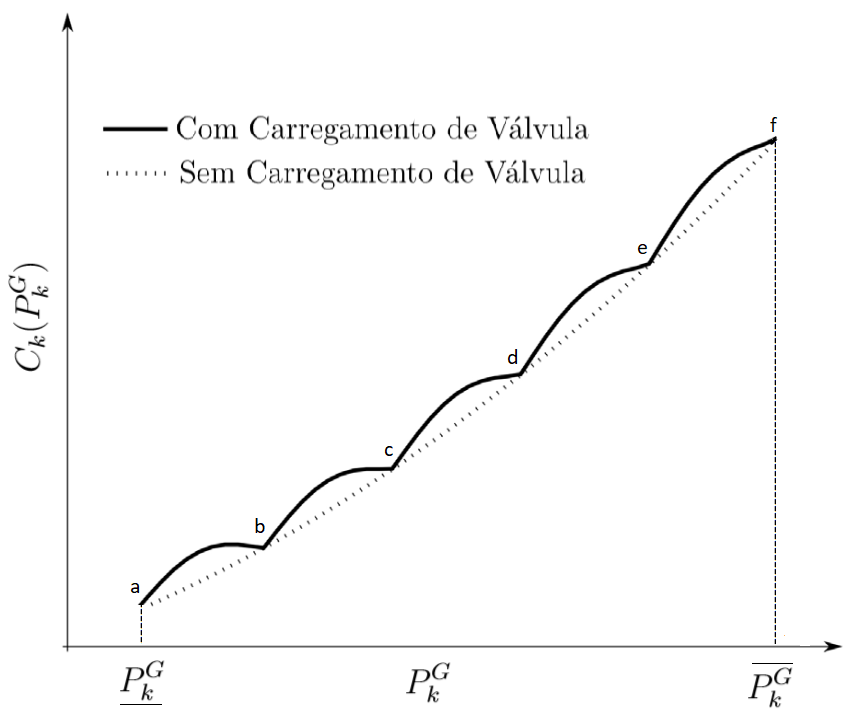
\includegraphics[width=100mm]{images/PCV2.png}
\fonte{Adaptado de \citeauthor{alawode} (2018).}
\label{FIGPCV}
\end{figure}


Para se obter uma função custo que seja mais representativa e considere o efeito de PCV, modifica-se a função (\ref{custoquad}) de modo que:

\begin{equation} \label{custopcv}
C_T(P^{G}) = \sum_{k \in \mathcal{G}} C_k(P^{G}_k) = \sum_{k \in \mathcal{G}} [a_k[P^{G}_k]^2 + b_kP^{G}_k + c_k + |e_k\sin(f_k[\underline{P^{G}_k}-P^{G}_k])|].
\end{equation}

Embora a função (\ref{custopcv}) seja mais completa e representativa do processo de geração em usinas termoelétricas, ela também acaba por introduzir novas dificuldades para o problema de otimização a ser resolvido. Devido ao fato da modelagem matemática do efeito de PCV ser realizada através de um valor absoluto senoidal, a função custo passa a ser não convexa e não diferenciável, impedindo a aplicação direta de métodos determinísticos de otimização \cite{dissertacaodiego}. Os pontos não diferenciáveis podem ser calculados pela equação (\ref{notdev}):

\begin{equation} \label{notdev}
P^{G}_{k} = \underline{P^{G}_{k}} - \frac{p\pi}{f_k},  \forall  p \in \Z.
\end{equation}

Neste trabalho, as restrições físicas e operacionais do SEP também serão consideradas na formulação matemática do problema DE-PCV-ZOP-RT, assim como no caso do FPOR. Portanto, as restrições de igualdade que representam os balanços de potência ativa (\ref{pot ativa}) e reativa (\ref{pot reativa}), as restrições de desigualdade dos limites de potência reativa  (\ref{lim reativa}) e magnitude de tensão (\ref{lim tensao}), e a natureza discreta dos \emph{taps} dos transformadores (\ref{tap}) e das susceptâncias equivalentes dos bancos de capacitores e reatores \emph{shunt} (\ref{shunt}), continuam sendo levadas em consideração. Por motivos de limitações físicas do sistema de geração, nem sempre é possível operar os geradores em todas as faixas de potência devido às eventuais vibrações nos rolamentos dos eixos das unidades geradoras e nas demais partes constituintes do sistema de geração \cite{abbas}. Consequentemente, a operação deve ser proibida em tais faixas de operação, ocasionando as restrições operacionais denominadas ZOP. As ZOP são descritas da seguinte forma:



% No entanto, no problema de DE-PCV-ZOP as potências ativas geradas também são variáveis, ao contrário do problema de FPOR onde eram consideradas como sendo constantes. Logo, torna-se necessário acrescentar a restrição de desigualdade referente aos limites máximos e mínimos de geração de potência ativa das unidades geradoras:

% \begin{equation} \label{lim potat}
% \underline{P^{G}_{k}} \leq P^{G}_{k} \leq \overline{P^{G}_{k}},\ \  \forall k \in \mathcal{G}.
% \end{equation}


\begin{equation} \label{ZOPEQ}
P^{G}_k \in ([\underline{P^{G}_k}, \overline{P^{G}_k}]-\cup_{j=1}^{n_k}[\underline{P^{G}_{k,j}}, \overline{P^{G}_{k,j}}]),
\end{equation}

\noindent em que $n_k$ é o número de total de zonas proibidas, $\underline{P^{G}_{k,j}}$ e $\overline{P^{G}_{k,j}}$ são os limites inferiores e superiores da \emph{k}-ésima unidade geradora na \emph{j}-ésima ZOP. A Figura \ref{FIGZOP} ilustra a curva de custo de geração de uma unidade geradora considerando as ZOP, os limites de geração e os efeitos de PCV.

Além dos efeitos de PCV e das ZOP, é comum encontrar na literatura outras representações relacionadas ao problema de DE, tais quais: as perdas calculadas através de um modelo matemático simplificado que utiliza os coeficientes-\emph{B} \cite{dissertacaodiego}, a utilização de múltiplos combustíveis (MC) \cite{kasma}, as restrições de taxa limite de rampa dos geradores (TLR) \cite{rampa} e a emissão de gases poluentes (EGP) \cite{PG-PSO-NR}. Neste trabalho, tais representações não serão levadas em consideração. Vale ressaltar que, na formulação matemática desenvolvida, as perdas estão inclusas nas equações do balanço de potência da representação do sistema elétrico.


\begin{figure}[!h]
\centering
\caption{Função custo com e sem representação dos efeitos de PCV e ZOP.}
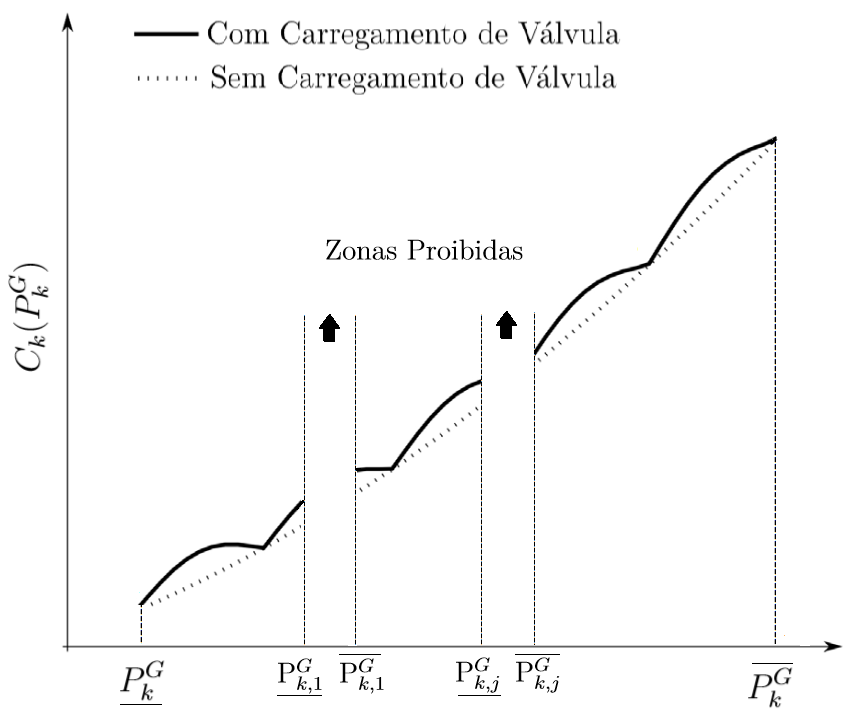
\includegraphics[width=100mm]{images/ZOP.png}
\fonte{Adaptado de \citeauthor{alawode} (2018).}
\label{FIGZOP}
\end{figure}

Tendo em vista o problema de DE em sua versão simplificada (\ref{de_classic}), modificando-se sua função objetivo para (\ref{custopcv}) e acrescentando-se as restrições de ZOP (\ref{ZOPEQ}) e da RT (\ref{pot ativa} - \ref{shunt}), pode-se expressar o modelo matemático do problema de DE-PCV-ZOP da seguinte maneira:

\begin{equation} \label{PCV-ZOP-FPO}
\begin{aligned}
\text{min}  &\quad C_T(P^{G})  \\
\text{s.a:} &\quad   \Delta P_k(V,\theta,t) = 0, \quad \forall k \in \mathcal{G}' \cup \mathcal{C} \\
&\quad   \Delta Q_k(V,\theta,t, b^{sh}) = 0, \quad \forall k \in \mathcal{C} \quad\\
&\quad P^{G}_k \in ([\underline{P^{G}_k}, \overline{P^{G}_k}]-\cup_{j=1}^{n_k}[\underline{P^{G}_{k,j}}, \overline{P^{G}_{k,j}}]), \quad \forall k \in \mathcal{G}, \quad j = 1,2,...,n_k\\
&\quad \underline{Q^{G}_{k}} \leq Q_{k}(V,\theta,t,b^{sh}) \leq \overline{Q^{G}_{k}}, \quad  \forall k \in \mathcal{G}\\
&\quad \underline{V_{k}} \leq V_{k} \leq \overline{V_{k}}, \quad  \forall k \in \mathcal{B}\\
&\quad b^{sh}_{k} \in D_{k}^{sh}, \quad \forall k \in \mathcal{B}^{sh}\\
&\quad t_{km} \in D_{km}^{tap},\quad \forall k,m \in \mathcal{T} \\
\end{aligned}
\end{equation}

Para fins de avaliação, no presente trabalho, o método híbrido proposto será aplicado ao problema de DE em dois casos de testes distintos: inicialmente, para o problema de DE (\ref{de_classic}) considerando apenas os efeitos de PCV e, em seguida, ao problema de DE considerando PCV, ZOP, RT, perdas, variáveis contínuas e discretas (\ref{PCV-ZOP-FPO}).

No próximo capítulo, será realizada a revisão bibliográfica do problema de FPO.

\section{Revisão Bibliográfica}

Nesta seção, será realizado um levantamento bibliográfico de trabalhos que foram desenvolvidos visando solucionar o problema de FPO, mais especificamente os subproblemas FPOR, DE e suas variantes. O objetivo é apresentar metodologias híbridas - compostas por métodos metaheurísticos e determinísticos - que já foram aplicadas na resolução destes problemas, visando contextualizar o método proposto neste trabalho. Por se tratarem de problemas não lineares, multimodais, restritos, descontínuos e não diferenciáveis, a maioria das técnicas utilizadas se baseiam em metaheurísticas, uma vez que são métodos flexíveis de fácil implementação e customização. Devido a tais características, ao longo dos anos, vem crescendo exponencialmente o número de pesquisas envolvendo computação evolutiva em aplicações do FPO \cite{metareview}.

A computação evolutiva é um ramo de pesquisa emergente da inteligência artificial - mais especificamente da inteligência computacional - que compreende um conjunto de algoritmos de busca e otimização inspirados na natureza, com ampla aplicação em aprendizado de máquina, redes neurais e problemas de otimização \cite{ec-ml, compint, rnn_evcomp}. Tais algoritmos apresentam um princípio de funcionamento de busca estocástica a partir da utilização de um grupo de agentes que representam soluções para o problema em questão, sendo, portanto, uma inteligência descentralizada, independente da diferenciabilidade do problema com excelente capacidade de realização de buscas globais no hiperespaço de soluções. Majoritariamente, podem ser divididos em quatro grupos distintos:

\begin{itemize}
    \item Algoritmos inspirados na evolução: simulam a evolução biológica e seus operadores de reprodução, mutação e seleção. Neste tipo de inteligência computacional, os agentes de busca representam indivíduos que são avaliados pelo seu \emph{fitness} (uma metáfora para com a capacidade de adaptação de um ser vivo na natureza). Quanto melhor sua avaliação, maior a probabilidade deste indivíduo se reproduzir e gerar melhores descendentes ao longo do processo iterativo. Exemplos de tais algoritmos são: DE \cite{de_}, GA \cite{ga_} e EP \cite{ep_};
    \item Algoritmos inspirados em inteligência de enxame: simulam o comportamento de espécies que convivem em sociedades ou bandos para otimizar algum critério necessário para sua sobrevivência. A principal característica deste tipo de algoritmo é a sua capacidade de compartilhamento de informação entre os agentes que o constituem, aprimorando, portanto, o processo de busca da solução. Como exemplo, pode-se citar: PSO \cite{pso_artigo} e otimização por colônia de formigas (do inglês \emph{ant colony optimization} ou ACO) \cite{aco};
    \item Algoritmos inspirados em fenômenos físicos: simulam as leis da natureza e comportamentos físicos ou químicos. Nestes algoritmos, os agentes se comunicam e movimentam-se com base em regras que são metáforas de conceitos científicos que regem o comportamento da natureza. São exemplos destes algoritmos: algoritmo de busca gravitacional (do inglês \emph{gravitational search algorithm} ou GSA) \cite{gsa} e recozimento simulado (do inglês \emph{simulated annealing} ou SA) \cite{Kirkpatrick1983OptimizationBS};
    
    
    \item Algoritmos de busca aleatória: são metaheurísticas sem inspiração em elementos da natureza. Baseiam-se em processos de busca aleatória no hiperespaço de soluções, geralmente utilizados para a realização de buscas locais. Exemplos destes algoritmos são: busca tabu (do inglês \emph{tabu search} ou TS) \cite{ts_} e procedimento de busca adaptável, aleatório e ambicioso (do inglês \emph{Greedy Randomized Adaptive Search Procedure} ou GRASP) \cite{grasp_}.

\end{itemize}


Além dos mencionados anteriormente, também pode-se encontrar na literatura, com menor frequência, outros tipos de algoritmos pertencentes ao ramo da inteligência computacional: sistemas imunes artificiais \cite{ais},  sistemas de lógica difusa (do inglês \emph{fuzzy systems}) \cite{fuzzy}, aprendizagem por reforço (do inglês \emph{reinforcement learning}) \cite{rl_}, dentre outros. Apesar de que em problemas não convexos e não diferenciáveis as metaheurísticas possuírem as vantagens citadas anteriormente em relação aos métodos determinísticos de otimização, pode-se citar como desvantagens:

\begin{itemize}
    \item Requerem um maior tempo computacional, uma vez que são métodos de busca baseados em grupos de agentes que se movimentam com um determinado grau de imprevisibilidade, exigindo um grande número de iterações e avaliações da função objetivo do problema;
    \item Apresentam performance sensível à escolha dos valores de seus hiperparâmetros, uma vez que a configuração adotada pode privilegiar uma busca global ou local. Assim, para achar a melhor configuração de hiperparâmetros para um determinado objetivo, torna-se necessário a execução de muitos testes computacionais;
    \item Impõem dificuldades na reprodutibilidade de testes e resultados, devido ao fato de possuírem processos e variáveis que assumem valores aleatórios durante sua execução;
    \item Apresentam uma degradação da performance conforme o número de dimensões (variáveis) dos problemas matemáticos aumentam;
    \item São métodos de otimização irrestritos, o que exige, em casos de problemas restritos, o tratamento das restrições através de mecânismos adicionais ou penalizações na função objetivo. As penalizações presentes na função \emph{fitness} são multiplicadas por constantes que ponderam suas respectivas forças, gerando uma dificuldade de se obter um balanço entre otimizar a função objetivo ou a factibilidade do problema.

\end{itemize}

Dentre todas as metaheurísticas aplicadas ao problema de FPO, destaca-se o algoritmo PSO - pertencente ao grupo dos algoritmos inspirados em inteligência de enxame - devido a grande quantidade de trabalhos e bons resultados encontrados na literatura a partir de sua utilização. Uma de suas principais vantagens é possuir uma maior objetividade no processo de busca aliada a um bom desempenho de otimização, acarretando em uma maior eficiência computacional. No entanto, apresenta como desvantagem, o fato de poder convergir prematuramente em problemas de grande porte e multimodais \cite{clpso}. Pensando nisso, milhares de pesquisas foram e vêm sendo desenvolvidas visando aprimorar a sua performance através de modificações da metaheurística original ou de hibridizações com métodos determinísticos e metaheurísticos. 

No presente trabalho, a revisão bibliográfica focará em métodos híbridos envolvendo a metaheurística PSO aplicados aos problemas de FPOR, DE e suas variantes. Uma extensa literatura da aplicação de metaheurísticas e suas modificações nos subproblemas de FPO pode ser encontrada nos trabalhos de: \citeonline{metareview}, \citeonline{abbas} e \citeonline{pso-ff}. A seguir, são apresentados os trabalhos híbridos envolvendo o algoritmo PSO.

\subsection{Abordagens Híbridas de Enxame de Partículas com Métodos Determinísticos}

Uma das combinações mais utilizadas pelos pesquisadores na literatura é a junção de metaheurísticas com métodos determinísticos de otimização. Neste tipo de hibridização, as metaheurísticas desempenham o papel de otimizador global enquanto que os métodos determinísticos realizam a otimização local. Tal combinação é poderosa pois une os pontos fortes de ambos os métodos de otimização.

Seguindo este raciocínio, \citeonline{PSO-SQP} propuseram um método que combina a metaheurística de PSO com o método determinístico SQP. Neste trabalho, os autores utilizam o método SQP embutido no interior do algoritmo de PSO, de forma que a cada iteração da metaheurística, executa-se o método determinístico para aprimorar a solução obtida pela partícula melhor avaliada do enxame. A abordagem híbrida desenvolvida foi aplicada no problema de DE com PCV considerando-se apenas as perdas calculadas a partir dos coeficientes-\emph{B} e os limites de geração de potência ativa, nos casos teste de 3, 13 e 40 geradores. O método híbrido proposto, em todos os casos de teste avaliados, obteve desempenho superior aos demais métodos metaheurísticos e híbridos utilizados para comparação. 

Em \citeonline{dynamic_pso_sqp}, os autores adaptaram o mesmo algoritmo desenvolvido em \citeyear{PSO-SQP} para uma variante do problema DE-PCV dinâmico, onde também leva-se em consideração a TLR, bem como as perdas calculadas através dos coeficientes-\emph{B}. O algoritmo híbrido preserva todas as características do primeiro trabalho, com exceção do peso de inércia da metaheurística que passa a ser considerado com decrescimento linear, ao invés de constante. As restrições de limite de rampa e da demanda também são tratadas como penalizações na função \emph{fitness} do algoritmo de PSO. O método foi aplicado em 3 casos de testes distintos. No primeiro caso, aplicou-se o método dinamicamente em um sistema de 10 geradores com uma curva de carga variável de hora em hora, neglicendiando-se as perdas de potência ativa. No segundo, utilizou-se o mesmo sistema, no entanto, foram consideradas as perdas bem como três curvas de carga distintas. No terceiro e último caso, o método foi aplicado para um sistema de 30 geradores, também com curva de carga variável. Em todos os casos, o algoritmo híbrido de PSO com SQP obteve resultados de custo médio e custo mínimo inferiores que as demais metaheurísticas e algoritmos híbridos utilizados para comparação. Os autores, em ambos os trabalhos, não mencionam qual a técnica utilizada para a aplicação do método SQP (que requer o cálculo do vetor gradiente para posterior aproximação da matriz hessiana pela técnica BFGS), uma vez que trata-se de um problema não diferenciável. Além disso, vale ressaltar que, nos problemas abordados, não foi levada em consideração a representação do sistema elétrico de transmissão.

\citeonline{pso_mpi_optimisation}, propuseram uma abordagem híbrida de enxame de partículas caótico (do inglês \emph{chaotic particle swarm optimization} ou CPSO) com o método de pontos interiores (MPI) para problemas de programação linear. O método é composto por duas etapas: na primeira, é executado o algoritmo CPSO visando realizar uma busca global no hiperespaço de soluções. Em seguida, na segunda etapa, as equações do problema são linearizadas e então é aplicado o MPI, como otimizador local. A metaheurística de CPSO possui praticamente os mesmos procedimentos que a versão original do PSO, no entanto, o peso de inércia é calculado por uma equação que insere uma maior estocacidade no comportamento das partículas. Durante seu funcionamento, as restrições de igualdade e desigualdade do problema são tratadas através da execução do FP e de penalizações na função \emph{fitness}, respectivamente. O método foi aplicado no sistema IEEE de 30 barras para minimização das perdas de potência ativa nas linhas de transmissão e apresentou melhores resultados quando comparado ao método PSO original. Embora os autores tenham dito levar em consideração as variáveis discretas, observa-se pelos dados disponibilizados que as soluções eram contínuas. O algoritmo híbrido em questão carece de mais comparações com outros métodos e de mais testes em sistemas de maior porte para uma melhor análise de sua eficiência.

\citeonline{PSO-QN}, desenvolveram um método híbrido que utiliza a metaheurística PSO com o método Quase-Newton denominado Broyden–Fletcher–Goldfarb–Shanno (BFGS). Na primeira etapa do método híbrido, a metaheurística é executada com a finalidade de realizar uma busca global no hiperespaço de soluções. Uma vez terminado este processo de busca, a solução encontrada é utilizada, na segunda etapa, como um ponto inicial para o método determinístico BFGS, que realiza uma busca local em sua vizinhança. O método foi aplicado no problema DE com PCV para o caso teste de 13 geradores, desconsiderando-se a representação da transmissão, eventuais perdas e ZOP. Embora a formulação matemática do problema abordado no trabalho leve em consideração os limites de geração de potência ativa dos geradores, os autores não mencionam qual a metodologia utilizada para tratá-los na metaheurística e no método determinístico, uma vez que ambos são métodos de otimização irrestritos.

Em \citeonline{psosugsakarn}, os autores também desenvolveram um método híbrido de PSO com SQP para resolução do problema de DE considerando PCV e MC. O algoritmo proposto é composto por duas etapas: na primeira, a metaheurística é executada para realizar uma busca global no hiperespaço de soluções. Na segunda, é executado o método determinístico partindo da solução encontrada pela etapa inicial. Foram realizados dois casos de teste no sistema de 10 geradores sem representação da transmissão e neglicenciando-se as perdas. No primeiro, foi considerado apenas a representação de MC. No segundo, além do MC, também foi considerado a representação de PCV. Embora os autores tenham obtido bons resultados nos testes efetuados, o trabalho não deixa claro qual a metodologia utilizada para tratar as restrições dos limites de geração, demanda e MC na metaheurística, nem a forma como é executado o método SQP considerando que trata-se de um problema descontínuo e não-diferenciável.


\citeonline{ep-pso-sqp}, propuseram um algoritmo híbrido das metaheurísticas PSO e EP com o método determinístico SQP. Neste método, os operadores do algoritmo EP são introduzidos no interior do algoritmo PSO para efetuar a geração, seleção e \emph{crossover} de indivíduos a cada iteração, de modo a aumentar a diversidade e a competitividade entre as partículas do enxame. A cada iteração, caso tenha havido melhoria no valor do \emph{fitness} da partícula melhor avaliada, executa-se o método SQP partindo de tal solução como ponto inicial. O método foi aplicado no problema DE dinâmico, com PCV e ZOP, sendo testado com curva de carga variável, nos casos com 3, 10, 15 e 30 geradores. Foram consideradas também as perdas calculadas através dos coeficientes-\emph{B}, as restrições de TLR e os limites de geração dos geradores, no entanto, o sistema de transmissão não foi representado. Os resultados dos testes realizados mostram que o algoritmo híbrido de EP com PSO e SQP obteve resultados melhores que os algoritmos híbridos EP com SQP e PSO com SQP, separados.

\citeonline{clpso3}, desenvolveram um método híbrido envolvendo a metaheurística CLPSO com o método determinístico SQP. O método determinístico é embutido no interior da metaheurística, sendo executado a partir de uma determinada iteração definida pelo usuário para aprimorar as três melhores partículas avaliadas do enxame. Testes computacionais foram realizados para os casos de 3, 13 e 40 unidades geradoras do problema de DE com PCV. Os autores não mencionam qual a técnica utilizada para o cálculo do gradiente da função objetivo que é não diferenciável, necessário para estimar a matriz hessiana pelo método quasi-newton mencionado no trabalho. Os resultados demonstram uma ligeira melhoria na otimização dos custos de geração dos sistemas para o método híbrido, em relação ao metodo CLPSO.

Em \citeonline{cpso_sqp}, os autores hibridizaram uma versão modificada da metaheurística de CPSO com o método de SQP. Neste método, é utilizado um peso de inércia adaptativo calculado com base nos valores dos \emph{fitness} individuais de cada partícula e nos valores de \emph{fitness} médio e mínimo do enxame. Além disso, a cada iteração, são utilizados dois processos de busca local: busca local caótica - baseada nas equações de Tent para sistemas caóticos - e o método SQP. Ambos são executados para a melhor partícula avaliada do enxame, no entanto, o método SQP é executado apenas se houver melhoria no \emph{fitness} de tal partícula em relação a iteração anterior. No fim de cada iteração, as cinco melhores partículas são mantidas no enxame, enquanto que as demais são recriadas em um espaço de busca reduzido ao redor da partícula melhor avaliada. Testes foram efetuados para o problema de DE com PCV nos casos de 3, 13 e 40 geradores. Foram consideradas as perdas calculadas através dos coeficientes-\emph{B} e os limites de geração de potência ativa dos geradores. As restrições do problema foram tratadas através de penalizações na função \emph{fitness}. Em todos os testes realizados a abordagem híbrida proposta alcançou os menores resultados de custos dentre todos os métodos utilizados como comparação. Os autores mostram que o método híbrido de CPSO com SQP apresenta uma velocidade de convergência superior ao da metaheurística CPSO, no entanto, pelas curvas plotadas, percebe-se que ambos tendem a convergir com um número de iterações inferior a 20\% do total, o que pode indicar uma convergência precoce a um mínimo local. 

\citeonline{pso_grad}, desenvolveram um algoritmo híbrido utilizando os métodos de otimização baseado em gradiente (do inglês \emph{gradient-based
optimization method} ou GM) e a metaheurística simples e aprimorada de otimização por inteligência de enxame (do inglês \emph{enhanced simplified swarm optimization} ou ESSOA). Nesta metaheurística, as partículas atualizam suas posições sem a necessidade de cálculo prévio da velocidade, utilizando apenas quatro outras referências: a sua posição anterior, a melhor posição individual de tal partícula no decorrer do algoritmo, a posição da melhor partícula do enxame e uma posição gerada aleatóriamente (respeitando-se os limites mínimos e máximos das variáveis independentes). Para superar o problema de convergência prematura do algoritmo, os autores adicionaram mecanismos de mutação das partículas e auto-adaptação dos parâmetros de controle da metaheurística. Para aprimorar a busca local, a cada iteração e para cada partícula, é executado o método GM a fim de minimizar uma função lagrangiana composta pelo custo de geração e pela diferença entre o somatório das potências geradas e a soma da demanda com as perdas. As partículas cujas posições estejam localizadas em pontos não diferenciáveis não são levadas em consideração na etapa de aplicação do GM, mantendo-as, portanto, fixas. Testes foram aplicados no problema de DE com PCV, ZOP, MC e TLR para os casos de 10, 15, 40 e 80 geradores, considerando as perdas calculadas através dos coeficientes-\emph{B}. O método apresentou bons resultados quando comparado a outras metaheurísticas e mostrou que a hibridização, juntamente com os mecanismos adotados, melhoraram o desempenho do algoritmo ESSOA.

Uma outra tentativa de hibridização utilizando a metaheurística clássica de PSO com o método determinístico de gradiente conjugado (GC) foi proposta por \citeonline{HPSO}. Assim como outros métodos híbridos, a metaheurística é utilizada como otimizador global e o método determinístico é embutido em seu interior como otimizador local (sendo executado para todas as partículas, a cada iteração). Os autores propõe duas variantes: na primeira, o método é GC executado para uma determinada partícula apenas se um número sorteado aleatoriamente - pertencente a uma distribuição uniforme $U(0,1)$ - for inferior ou igual a uma probabilidade predefinida. Na segunda, é criada uma lógica condicional que estabelece um número mínimo e máximo de vezes que cada partícula pode ser utilizada para execução do método GC. Os autores constataram que o desempenho da segunda variante é melhor, uma vez que no primeiro caso algumas partículas podem correr o risco de não serem utilizadas como ponto inicial do método determinístico, de modo que a exploração local em determinadas regiões nunca seja realizada. Além disso, estabelecer um número máximo de execuções da busca local para as partículas diminui o tempo computacional requerido pelo algoritmo. Ambas as variantes propostas foram testadas nos casos de 6, 13 e 38 geradores para o problema de DE, levando em consideração os efeitos de PCV, ZOP e TLR, assim como as perdas calculadas através dos coeficientes-\emph{B}. Analisando o desempenho da abordagem proposta em relação a outras metaheurísticas e algoritmos híbridos, observa-se um desempenho competitivo no custo mínimo e médio obtidos. No entanto, ao se analisar as curvas de convergência da metaheurística, observa-se que o valor mínimo de custo é obtido ao se executar menos de 10\% do total das iterações, o que pode indicar uma convergência prematura. Os autores não detalham o funcionamento do método determinístico GC, nem como as restrições do problema são tratadas pela metaheurística. 


\citeonline{pso_mpi}, propuseram uma abordagem híbrida MPI com o algoritmo de PSO para a resolução do problema de FPOR, visando minimizar as perdas de potência ativa nas linhas de transmissão. No trabalho em questão, o MPI é executado para resolver o problema em sua forma relaxada, onde todas as variáveis são consideradas como sendo contínuas. Em seguida, a solução encontrada pelo método determinístico é utilizada como sendo uma das partículas do enxame da metaheurística de PSO, que realiza uma busca na vizinhança deste ponto. Nesta etapa, são otimizadas apenas as variáveis de controle discretas (\emph{taps} e susceptâncias \emph{shunt}). O método foi aplicado no sistemas elétricos Dinamarquês Ocidental de 400 barras e IEEE de 39 barras. Os autores não mencionam quais as metodologias utilizadas na metaheurística para tratar as restrições operacionais do sistema e as variáveis discretas. Foi demonstrado que a hibridização destes algoritmos, na ordem proposta, pode alcançar soluções de melhor qualidade que o simples processo de arredondamento da solução contínua do MPI, aumentanto também as chances de convergência. No entanto, vale ressaltar que, para problemas multimodais, a utilização do método determinístico em uma etapa inicial do algoritmo pode acarretar em uma convergência precoce para um ponto de mínimo local distante do mínimo global do problema, de forma que, na segunda etapa, a busca
efetuada pela metaheurística acabe sendo realizada em uma região não promissora.


\subsection{Abordagens Híbridas de Enxame de Partículas com Métodos Metaheurísticos}

Outra modalidade comum de hibridização é a junção entre metaheurísticas. Neste caso, é comum a utilização de uma metaheurística para realizar a otimização global e outra para realizar a otimização local. Além desse tipo de combinação, também é possível encontrar algoritmos que misturam os operadores de uma ou mais metaheurísticas, visando o aperfeiçoamento da performance em algum critério específico desejado.

Inspirado no processo físico de recozimento de metais, \citeonline{pso-sa} propuseram uma combinação das metaheurística PSO e SA para resolução do problema de DE com PCV, TLR, ZOP e perdas calculadas através dos coeficientes-\emph{B}. Neste método, os parâmetros do PSO e SA são inicializados, bem como cada partícula é inicializada aleatoriamente. Então, calcula-se o seu valor de \emph{fitness}, sua velocidade e sua nova posição. Verifica-se se houve melhoria no valor do \emph{fitness} em relação à iteração anterior ou se a diferença do \emph{fitness} atual para o anterior, dividida por uma ``temperatura$"$ predefinida, é inferior a um número aleatoriamente sorteado de uma distribuição uniforme $U(0,1)$. Em caso afirmativo, o algoritmo segue para a próxima iteração, atualizando os valores de peso de inércia, temperatura, memórias das partículas e a partícula melhor avaliada do enxame. Em caso negativo, novas velocidades e posições são calculadas para as partículas e repete-se o processo de verificação da melhoria do \emph{fitness}. A cada iteração, a ``temperatura$"$ é diminuída simulando o processo de resfriamento do algoritmo de SA, sendo, portanto, a responsável por controlar o quanto as partículas divergem no decorrer das iterações. Testes foram realizados para os casos de 6, 15 e 40 geradores, demonstrando que o algoritmo obteve resultados melhores que as metaheurísticas de GA, PSO e SA, individualmente. As restrições do problema são tratadas através de penalizações na função \emph{fitness} e a RT não foi considerada.

\citeonline{pso-ma}, propuseram uma combinação das metaheurísticas PSO com sistemas multiagentes (do inglês \emph{multiagent systems} ou MAS) e GA. Nesta metodologia, inicialmente, as partículas são criadas aleatoriamente respeitando-se os limites do hiperespaço de busca. Em seguida, para todas, é executado o algoritmo de Newton-Raphson (NR) para resolução do FP, permitindo, então, o cálculo da função \emph{fitness}. Uma vez determinado o valor de seu \emph{fitness}, cada partícula passa por um procedimento de busca local em sua vizinhança através dos operadores de cooperação e competição do método MAS. Então, as partículas resultantes com piores avaliações sofrem as ações de \emph{breeding} e \emph{subpopulation} da metaheurística GA.  Em seguida, para o novo enxame atualizado, são calculadas as novas velocidades e novas posições das partículas. O processo iterativo repete-se até que o critério de parada estabelecido seja satisfeito. O algoritmo desenvolvido foi aplicado para o problema de FPOR visando a minimização das perdas nos sistemas IEEE de 30 e 118 barras, apresentando bons resultados na redução das perdas e no tempo computacional de execução em relação as outras metaheurísticas e algoritmos híbridos utilizados como comparação. Apesar dos bons resultados, vale ressaltar que os autores não levam em consideração a existência da variáveis discretas na formulação matemática do problema.

No trabalho de \citeonline{pso-ga-sc1}, um operador de mutação da metaheurística GA é adicionado ao algoritmo de PSO, visando um aumento na diversificação das partículas do enxame. A cada iteração, após a atualização das velocidades e posições do enxame, seleciona-se um determinado número de partículas - sujeitas a uma probabilidade predefinida - para sofrerem mutação. Ao selecionar determinada partícula, um vetor de números binários de mesmo tamanho é gerado aleatoriamente, onde as posições com presença do número ``1$"$ indicam a variável da partícula que irá ser mutada. O procedimento descrito anteriormente repete-se até que o critério de parada do algoritmo de PSO seja satisfeito. Na abordagem proposta, foram testadas diferentes variantes do algoritmo PSO, sendo que a com peso de inércia e fator de constrição apresentou melhores resultados nas funções de \emph{benchmark}. O método foi aplicado em dois casos de teste: DE com PCV e MC para um sistema de 10 geradores e DE com PCV para um sistema de 40 geradores. Para lidar com a restrição da demanda, os autores propõem uma heurística iterativa que realiza pequenos acréscimos ou decréscimos nas potências de cada gerador, para cada partícula, mantendo-se sempre as variáveis dentro de seus limites operacionais. Nos testes realizados, o método híbrido apresentou desempenho competitivo entre os demais algoritmos comparados, destacando-se sempre entre os melhores resultados. Observa-se, pelas curvas de convergência plotadas, que o método apresenta menor susceptibilidade de convergir prematuramente a um mínimo local do problema. Melhores resultados poderiam ter sido alcançados se algum mecanismo de busca local também tivesse sido implementado.


\citeonline{pso-de}, implementaram um algoritmo híbrido das metaheurísticas PSO e ED. Nesta abordagem, os operadores de atualização das velocidades e posições das partículas são embutidos no interior da metaheurística ED. Inicialmente, é inicializada aleatoriamente uma população ``mãe$"$  de indivíduos e, em seguida, são criadas duas outras populações provisórias: uma através do operador de mutação original da metaheurística de ED, e outra através dos operadores de atualização das velocidades e posições da metaheurística PSO. Então, as populações provisórias passam por um procedimento de \emph{crossover} dando origem a duas populações ``filhas$"$. Uma vez que todos os indivíduos tenham sido avaliados, é executado um procedimento de seleção entre as populações ``filhas$"$ e ``mãe$"$, mantendo-se aqueles com o melhor \emph{fitness}. Segundo os autores, a abordagem promove uma maior diversificação dos indivíduos presentes na população, evitando a convergência precoce para um mínimo local do problema. Testes computacionais foram realizados para o problema de DE em três casos distintos: o primeiro, considerando-se os efeitos de PCV em um sistema de 40 geradores. O segundo, considerando-se as perdas calculadas pelos coeficientes-\emph{B}, ZOP e TLR, para um sistema de 15 geradores. O teceiro, considerando-se os efeitos de PCV e MC, para um sistema de 10 geradores. Em todos os casos, as restrições do problema são tratadas através da penalização na função \emph{fitness}. O método proposto obteve um excelente desempenho dentre todas as comparações realizadas com outras metaheurísticas e algoritmos híbridos. Vale ressaltar que os autores não levaram em consideração as restrições de RT. Um ponto negativo do algoritmo proposto é a necessidade de ter de avaliar duas populações de indivíduos a cada iteração, o que pode ser computacionalmente dispendioso.


Um algoritmo híbrido envolvendo as metaheurísticas PSO e GSA - que simula a teoria da gravitação universal elaborada por Newton - foi proposto por \citeonline{pso-gsa}. Neste algoritmo, inicialmente, todos as partículas ou massas são inicializadas aleatoriamente dentro dos limites permitidos para cada variável do problema. Em seguida, cada partícula é avaliada pela função \emph{fitness} e, então, são definidas suas ``massas$"$ e calculadas as forças e acelerações resultantes entre as partículas do enxame, onde as ``massas$"$ são proporcionais à qualidade do \emph{fitness} e as forças entre as partículas proporcionais às massas e às distâncias entre elas. A atualização das velocidades e posições das partículas é realizada assim como no algoritmo de PSO, no entanto, a parcela referente ao aspecto cognitivo (diferença entre a atual posição e a memória individual da partícula) é substituída pela aceleração anteriormente calculada. Para aprimorar os processos de exploração global e local, os autores propuseram um limite máximo de velocidade que se auto-ajusta a cada iteração, de acordo com um conjunto de regras de um sistema \emph{fuzzy}, que utiliza como dados de entrada informações sobre o melhor \emph{fitness} do enxame. Testes foram realizados para o problema de DE com PCV nos casos de 13 e 40 geradores, e nos sistemas de 14 e 30 barras do IEEE - considerando as perdas calculadas através dos coeficientes-\emph{B}. Embora os autores não tenham considerado a RT, os resultados alcançados demonstraram ser excelentes na vasta comparação realizada com outras metaheurísticas e métodos híbridos. 

\citeonline{pso-aco}, implementaram um algoritmo híbrido com as metaheurísticas PSO e ACO, que simula o comportamento das formigas na construção de rotas de busca por alimento. Na abordagem proposta os autores utilizaram as metaheurísticas em duas etapas: na primeira, é executado o algoritmo de PSO até que o número total de iterações seja satisfeito. Uma vez terminado, a solução encontrada é passada ao algoritmo ACO como uma das formigas iniciais da colônia. Nesta abordagem, as potências dos geradores são discretizadas e simbolizam vértices de um grafo, interligados pelos caminhos. A cada iteração, novas formigas percorrem tais caminhos depositando feromônios de acordo com a qualidade do \emph{fitness} obtido, de forma que quanto mais feromônios depositados, maior a probabilidade do caminho ser selecionado. Se o caminho é pouco frequentado, o feromônio depositado tende a evaporar. No final do algoritmo, o caminho com maior quantidade feromônios é a solução do problema. Os autores aplicaram o algoritmo em quatro casos de teste: DE, DE com PCV, DE com PCV e TLR e, por fim, DE com PCV e POZ - todos para um sistema simples de 6 geradores. Em todos os casos o método proposto obteve bons resultados quando comparados a outras metaheurísticas e aos algoritmos PSO e ACO, individualmente. Apesar de bons, os autores aplicaram o algoritmo em um sistema de pequeno porte sem RT e não informaram detalhes do algoritmo híbrido, como: número de discretizações das potências dos geradores e modo de tratamento das restrições do problema.


Em \citeonline{pso_gwo_de}, os autores desenvolveram método híbrido a partir da junção de duas metaheurísticas: PSO e otimização por alcateia de lobos cinzentos (do inglês \emph{grey wolf optimization} ou GWO), que simula o processo de caça de lobos. Nesta hibridização, o algoritmo de PSO é embutido no interior do GWO, de forma que a cada iteração os lobos da alcateia são passados à metaheurística de PSO como sendo partículas. Após a execução completa do algoritmo de PSO, tais partículas retornam ao algoritmo original de GWO como sendo lobos. Então, são calculados os novos \emph{fitness} e atualizadas as posições dos novos lobos. O processo se repete até que o número máximo de iterações do GWO seja atingido. O método foi aplicado no problema de DE considerando as perdas calculadas através dos coeficientes-\emph{B}, para os casos de 3 e 6 unidades geradoras. Em comparação com a metaheurística GWO pura, o método híbrido apresenta uma velocidade de convergência superior. No entanto, vale ressaltar que, o método pode ser dispendioso computacionalmente uma vez que para cada iteração do GWO é executado o algoritmo PSO em sua totalidade. Além disso, sabe-se que no decorrer das iterações da metaheurística PSO as partículas tendem a se aproximar conjuntamente da melhor solução, de forma que ao retornar tal enxame ao algoritmo de GWO como sendo os novos lobos, teremos uma alcateia pouco diversificada e com espaço de busca reduzido, podendo gerar convergência prematura a um mínimo local do problema.

\citeonline{pso-ga-sc2}, propuseram uma combinação da metaheurística de enxame de partículas modificada (do inglês \emph{modified particle swarm optimization} ou MPSO) com GA. Inicialmente, o algoritmo tradicional de GA é executado para uma população de indivíduos aleatoriamente criada, contendo os operadores de mutação, \emph{crossover} e seleção. Em seguida, um terço das melhores partículas é selecionado para estar no enxame inicial do algoritmo MPSO. No algoritmo MPSO, um novo operador para criação aleatória de partículas é proposto, sendo que a cada iteração são mantidas apenas um terço das melhores partículas do enxame e as demais são recriadas utilizando tal operador. Testes foram realizados para o problema de DE com PCV, ZOP, MC e TLR, nos casos de 6, 10 e 15 geradores, considerando as perdas calculadas através dos coeficientes-\emph{B}. Embora o algoritmo tenha apresentado bons resultados em comparação a outras metaheurísticas, sua aplicação ficou restrita a sistemas de pequeno porte sem a RT.

Um método híbrido envolvendo as metaheurísticas PSO e TS foi desenvolvido por \citeonline{PSO-TS}. Nesta abordagem, a metaheurística de PSO é utilizada como otimizador global, enquanto que o algoritmo TS é utilizado como otimizador local. A metaheurística TS é embutida no interior do algoritmo de PSO, sendo executada a cada iteração para aprimorar localmente a memória de cada partícula do enxame (que contém a melhor localização pela qual a partícula já esteve até então), explorando sua vizinhança. A vizinhança a ser explorada pelo método TS é definida através da técnica denominada hiper-retângulo, que seleciona aleatoriamente pontos que estão no interior de um hiperespaço centralizado na posição da memória da partícula e que se estende até um determinado raio predefinido pelo desenvolvedor. Os critérios de parada adotados para tal etapa são: o número total de iterações e o número de iterações sem melhorias no \emph{fitness} da memória. Caso este processo acarrete em melhoria do \emph{fitness} da memória, esta é atualizada no algoritmo de PSO para seu novo valor. Em seguida, após a exploração local, retorna-se o fluxo original do algoritmo PSO até que o número máximo de iterações seja atingido. O método híbrido foi aplicado no problema de FPOR no sistema de 30 barras do IEEE para a minimização das perdas de potência ativa e desvio de tensão. As restrições de igualdade e desigualdade do problema são tratadas pela resolução do FP e por penalizações na função \emph{fitness}, respectivamente. Embora os autores tenham aplicado o método apenas em um sistema de pequeno porte e não tenham levado em consideração a presença de variáveis discretas, ele apresentou bom desempenho quando comparado a outras metaheurísticas e aos próprios métodos PSO e TS, isoladamente. 
 
No trabalho de \citeonline{pso-ff}, é proposta uma hibridização entre a metaheurísticas PSO e algoritmo do vaga-lume (do inglês \emph{firefly algorithm} ou FA), que simula o processo de comunicação de tais insetos através do fenômeno de bioluminescência. Na abordagem proposta, o método PSO é utilizado como otimizador global e o método FA como otimizador local. Inicialmente, inicializa-se um enxame de partículas aleatoriamente respeitando-se os limites do hiperespaço de busca. Em seguida, para cada partícula é resolvido o FP e calculado seu \emph{fitness}. Sempre que uma partícula obtiver melhoria no valor de seu \emph{fitness} em relação à iteração anterior, sua posição e velocidade serão calculadas utilizando as equações da metaheurística FA. Caso contrário, são utilizadas as equações da metaheurística de PSO. Para aprimorar o desempenho do algoritmo de PSO, os autores desenvolveram um sistema \emph{fuzzy} para ajustar automaticamente os coeficientes de aceleração individuais de cada partícula, com base em seu valor de \emph{fitness} e no número da respectiva iteração. Testes foram realizados nos sistemas elétricos de 30, 57 e 118 barras do IEEE, para o problema de FPOR considerando quatro diferentes casos: as perdas de potência ativa, o desvio de tensão, o índice de estabilidade de tensão e, por fim, um caso multiobjetivo. As restrições de igualdade e desigualdade do problema foram tratadas através da resolução do FP e de penalizações na função \emph{fitness}, respectivamente. Em todos os casos de teste a abordagem híbrida proposta se sobressaiu em relação as outras metaheurísiticas utilizadas para comparação, mantendo também um tempo computacional competitivo.


Em \citeonline{pso_gwo}, os autores propuseram um algoritmo híbrido de PSO com GWO com a mesma configuração implementada por \citeonline{pso_gwo_de}. No entanto, testes computacionais foram realizados nos sistemas elétricos de 14, 30 e 118 barras do IEEE, para o problema de FPOR. Para cada sistema teste, foram implementadas e estudadas duas funções objetivos: a minimização das perdas de potência ativa nas linhas de transmissão e a minimização do desvio de tensão nas barras. As restrições do problema são tratadas através da penalização na função \emph{fitness} das metaheurísticas. O método proposto obteve melhores resultados que as demais metaheurísticas utilizadas para comparação, em ambos os casos de teste. Assim como no trabalho de \citeonline{pso_gwo_de}, a configuração escolhida para combinar as metaheurísticas pode acabar se tornando um ponto fraco da abordagem proposta, tendo em vista os problemas mencionados anteriormente sobre o tempo computacional e a convergência prematura.


\subsection{Análise Geral}

Nesta seção, será realizada uma análise geral da revisão da literatura efetuada anteriormente. Sabe-se, que os métodos determinísticos de otimização possuem dificuldades em performar de modo eficiente em problemas não-convexos e multimodais, embora sejam excelentes ferramentas para a efetuação de buscas locais. Além disso, precisam englobar técnicas matemáticas auxiliares para poderem lidar com a não-diferenciabilidade da função objetivo e com a presença de variáveis discretas. Por outro lado, as metaheurísticas, embora sejam uma boa opção para a realização de buscas globais no hiperespaço de soluções, apresentam dificuldades em problemas do tipo restritos de larga escala. O problema de FPO, por sua vez, possui todas as características e empecilhos citados anteriormente, dificultando a aplicação de ambos os métodos de otimização em sua resolução. 

Como visto anteriormente, a metaheurística de PSO, embora tenha um grande destaque em aplicações do FPO, apresenta como principal ponto negativo a possibilidade de convergência prematura \cite{clpso}. Além disso, por se tratar de um algoritmo de busca estocástico, carece da capacidade de efetuar buscas locais efetivas no hiperespaço de soluções quando comparadas aos métodos determinísticos de otimização. De forma geral, as hibridizações visam corrigir ambos os aspectos em seu funcionamento. Uma síntese do levantamento bibliográfico realizado, em ordem cronológica, pode ser encontrada nas Tabelas \ref{Tabela1} e \ref{Tabela2}. 

\begin{table}[h!]

\centering
\caption{\label{Tabela1}Algoritmos híbridos de PSO com métodos determinísticos para resolução dos subproblemas do FPO.}

\begin{tabular}{cccc}
	\hline
	\textbf{Métodos Híbridos} & \textbf{\makecell{Problemas\\(Objetivos)}} & \textbf{\makecell{Sistemas \\ Elétricos}} & \textbf{\makecell{Variáveis \\ Discretas}}  \\ \hline
	
% 	\makecell{GA-MPI\\\citeonline{ga_ip_pt}} & \makecell{FPOR\\($P_L$)}    & 
% 	\makecell{GO-DF e \\ IEEE 118}  & Sim    \\ \hline
	
% 	\makecell{EP-SQP\\\citeonline{EP-SQP}} & \makecell{DE-PCV\\($C_T$)}    & 
% 	\makecell{-}  & Não    \\ \hline
	
%     \makecell{GA-MPI\\\citeonline{ga_ip}} & \makecell{FPOR\\($P_L$)}    & 
%     \makecell{IEEE 30, IEEE 118\\e Chongqi}  & Sim    \\ \hline
    
    \makecell{PSO com SQP\\\tiny\cite{PSO-SQP}} & \makecell{DE com PCV\\($C_T$)}    & 
	\makecell{-}  & Não    \\ 
	
    \makecell{PSO com SQP\\\tiny\cite{dynamic_pso_sqp}} & \makecell{DE com PCV e TLR\\($C_T$)}    & 
	\makecell{-}  & Não    \\ 
	
    \makecell{PSO com MPI\\\tiny\cite{pso_mpi_optimisation}} & \makecell{FPOR\\($P_L$)}    & 
	\makecell{IEEE 30}  & Não    \\ 
	
	
    \makecell{PSO com BFGS\\\tiny\cite{PSO-QN}} & \makecell{DE com PCV\\($C_T$)}    & \makecell{-}  & Não    \\ 
    % \makecell{MPI-EP\\\citeonline{PE-IP}} & \makecell{FPOR\\($P_L$)}    & 
    % \makecell{IEEE 118\\e Chongqi}  & Sim \\ \hline

    % \makecell{PSO Discreto\\\citeonline{psohibrido}} & \makecell{DE com PCV e RT\\($C_T$, $EGP$ e $P_L$)}    & \makecell{IEEE 30}  & Sim    \\ \hline

    % \makecell{MPI-ED\\\citeonline{IP-DE}} & \makecell{DE-PCV\\($C_T$)}    & \makecell{-}  & Não    \\ \hline


    \makecell{PSO SQP\\\tiny\cite{ep-pso-sqp}} &  \makecell{DE com PCV e MC\\($C_T$)}   & \makecell{-}  & Não    \\ 

    \makecell{PSO com EP e SQP\\\tiny\cite{ep-pso-sqp}} &  \makecell{DE com PCV,\\ZOP e TLR\\($C_T$)}   & \makecell{-}  & Não    \\
    \makecell{CPSO com SQP\\\tiny\cite{cpso_sqp}} &  \makecell{DE com PCV\\($C_T$)}   & \makecell{-}  & Não    \\ 
    
    \makecell{CLPSO com SQP\\\tiny\cite{clpso3}} &  \makecell{DE com PCV\\($C_T$)}   & \makecell{-}  & Não    \\
    \makecell{CPSO com SQP\\\tiny\cite{cpso_sqp}} &  \makecell{DE com PCV\\($C_T$)}   & \makecell{-}  & Não    \\ 


    \makecell{ESSOA com GM\\\tiny\cite{pso_grad}} &  \makecell{DE com PCV, ZOP\\MC e TLR\\($C_T$)}   & \makecell{-}  & Não    \\ 

    \makecell{PSO com GC \\\tiny\cite{HPSO}} &  \makecell{DE com PCV,\\ZOP e TLR\\($C_T$)}   & \makecell{-}  & Não    \\ 

    \makecell{PSO com MPI\\\tiny\cite{pso_mpi}} &  \makecell{FPOR\\($P_L$)}   & \makecell{IEEE 39 e\\Dinamarquês\\Ocidental}  & Sim    \\ 
    
    % \makecell{PG-FC-PSO\\\citeonline{PG-PSO-NR}} &  \makecell{DE com RT\\($C_T$ e $EGP$)}   & \makecell{IEEE 30}  & Não    \\ \hline
    
    \hline
    
\end{tabular}
\fonte{Autor.}
\end{table}

\begin{table}[h]

\centering
\caption{\label{Tabela2}Algoritmos híbridos de PSO com metaheurísticas para resolução dos subproblemas do FPO.}

\begin{tabular}{cccc}
	\hline
	\textbf{Métodos Híbridos} & \textbf{\makecell{Problemas\\(Objetivos)}} & \textbf{\makecell{Sistemas \\ Elétricos}} & \textbf{\makecell{Variáveis \\ Discretas}}  \\ \hline
	
\makecell{PSO com SA\\\tiny\cite{pso-sa}} &  \makecell{DE com PCV,\\ ZOP e TLR\\($C_T$)}   & \makecell{-}  & Não    \\
    
    \makecell{PSO com MAS e GA\\\tiny\cite{pso-ma}} &  \makecell{FPOR\\($P_L$)}   & \makecell{IEEE 30 e\\
    118}  & Não    \\ 
    
    \makecell{PSO com AG \\\tiny\cite{pso-ga-sc1}} &  \makecell{DE com PCV e MC\\($C_T$)}   & \makecell{-}  & Não    \\ 
    
    \makecell{PSO com ED\\\tiny\cite{pso-de}} &  \makecell{DE com PCV, ZOP\\ MC e TLR\\($C_T$)}   & \makecell{-}  & Não    \\ 
    
    
    \makecell{PSO com GSA\\\tiny\cite{pso-gsa}} &  \makecell{DE com PCV\\($C_T$)}   & \makecell{-}  & Não    \\ 
    

    \makecell{PSO com GWO\\\tiny\cite{pso_gwo_de}} &  \makecell{DE\\($C_T$)}   & \makecell{-}  & Não    \\ 
    % \makecell{ALO-NR\\\citeonline{antlion}} &  \makecell{FPOR\\($P_L$, $DT$ e $IET$)}   & \makecell{-}  & Não    \\ \hline

    \makecell{PSO com ACO\\\tiny\cite{pso-aco}} &  \makecell{DE com PCV, ZOP\\e TLR($C_T$)}   & \makecell{-}  & Não    \\ 
    % \makecell{ALO-NR\\\citeonline{antlion}} &  \makecell{FPOR\\($P_L$, $DT$ e $IET$)}   & \makecell{-}  & Não    \\ \hline 
    
    \makecell{MPSO com GA\\\tiny\cite{pso-ga-sc2}} &  \makecell{DE com PCV, ZOP\\MC e TLR\\($C_T$)}   & \makecell{-}  & Não    \\ 
    % \makecell{ALO-NR\\\citeonline{antlion}} &  \makecell{FPOR\\($P_L$, $DT$ e $IET$)}   & \makecell{-}  & Não    \\ \hline 
    
    \makecell{PSO com TS\\\tiny\cite{PSO-TS}} &  \makecell{FPOR\\($P_L$ e $DT$)}   & \makecell{IEEE 30}  & Não    \\
    % \makecell{ALO-NR\\\citeonline{antlion}} &  \makecell{FPOR\\($P_L$, $DT$ e $IET$)}   & \makecell{-}  & Não    \\ \hline 
    
    \makecell{PSO com FA\\\tiny\cite{pso-ff}} &  \makecell{FPOR\\($P_L$, $DT$ e $IET$)}   & \makecell{IEEE 30, 57\\e 118}  & Não    \\ 
       
    \makecell{PSO com GWO\\\tiny\cite{pso_gwo}} &  \makecell{FPOR\\($P_L$ e $DT$)}   & \makecell{IEEE 14, 30\\e 118}  & Não    \\ 
    % \makecell{ALO-NR\\\citeonline{antlion}} &  \makecell{FPOR\\($P_L$, $DT$ e $IET$)}   & \makecell{-}  & Não   \hline
    \hline
\end{tabular}
\fonte{Autor.}
\end{table}

Uma das principais arquiteturas utilizadas em algoritmos híbridos é a inserção de um método determinístico no interior da metaheurística, de forma que este é executado a cada iteração ou a partir de uma determinada condição estabelecida pelo desenvolvedor para aprimorar a qualidade da solução de um ou mais agentes de busca. Pode-se destacar dois aspectos como pontos negativos desta abordagem: em primeiro lugar, o tempo computacional aumenta consideravelmente pois o método determinístico é executado um grande número de vezes. Em segundo lugar, pelo fato da metaheurística utilizar penalizações para tratar das restrições do problema matemático, uma possível solução local e factível encontrada pelo método determinístico acabaria levando vantagem em relação aos demais agentes de busca que se movimentam de forma aleatória e a todo momento são penalizados. Algumas metaheurísticas tendem a ser mais propensas a direcionar o processo de busca na direção do agente melhor avaliado da população, o que pode acarretar em uma convergência precoce a um mínimo local em problemas multimodais e não convexos. 

De forma similar à arquitetura mencionada anteriormente, frequentemente são utilizadas metaheurísticas secundárias para a realização da exploração local ao redor dos agentes de busca da metaheurística primária. Também pode-se destacar como ponto negativo desta abordagem o tempo computacional requerido, uma vez que metaheurísticas não possuem a mesma eficiência que métodos determinísticos na realização de buscas locais. Além disso, o número de diferentes possíveis soluções cresce exponencialmente com o número de variáveis, de forma a precarizar o desempenho de métodos de buscas estocásticos em problemas de maior porte \cite{high_dim, maldicao}. 

Encontra-se também na literatura a arquitetura híbrida que executa inicialmente um método determinístico e utiliza sua solução como um dos agentes da metaheurística a ser executada em uma segunda etapa, procedimento comumente denominado ``boa-partida$"$ (do inglês \emph{warm-start}). Um ponto negativo desta abordagem é o fato de que, em problemas não convexos, a solução inicial encontrada pelo método determinístico pode ser um mínimo local localizado distante da solução ótima global do problema, direcionando os agentes de busca da metaheurística a uma região não promissora do hiperespaço de soluções.

A mesclagem de operadores de diferentes metaheurísticas também é uma das soluções encontradas pelos pesquisadores com o propósito de aprimorar as capacidades de exploração local ou global dos algoritmos híbridos. Em específico ao caso do PSO, comumente se utilizam operadores que visam aprimorar a capacidade de diversificação do enxame, minimizando as chances do algoritmo convergir prematuramente a um mínimo local do problema. Por outro lado, o algoritmo tende a perder objetividade e a capacidade de efetuar explorações locais.

Por último, mas não menos importante, há a arquitetura híbrida que utiliza os algoritmos metaheurísticos e determinísticos em duas etapas distintas: inicialmente, a metaheurística realiza uma exploração global à procura de uma solução ótima e, em seguida, tal solução é utilizada como ponto inicial (\emph{warm-start}) do método determinístico que realiza um aperfeiçoamento de sua qualidade. Nesta arquitetura, pode-se encontrar também métodos metaheurísticos substituindo o papel realizado pelos métodos determinísticos, no entanto, como destacado anteriormente, a eficiência não acaba sendo equivalente. Alguns autores podem ainda utilizar um método exato no interior da metaheurística para ajudá-la com as restrições do problema, como é o caso dos algoritmos híbridos que utilizam um método determinístico para a resolução do FP, diminuindo também o número de restrições e variáveis com as quais as metaheurísticas teriam de lidar.


Neste resumo, estão enfatizados os algoritmos utilizados nas metodologias híbridas, bem como os problemas considerados e suas respectivas funções objetivos, os sistemas elétricos utilizados e a presença ou não de variáveis discretas. Observa-se, pelas Tabelas \ref{Tabela1} e \ref{Tabela2}, que na maioria dos casos os pesquisadores não levam em consideração a RT e, consequentemente, a presença de variáveis discretas. A RT torna o problema de FPO extremamente restrito, devido as equações que representam as restrições dos balanços de potência ativa (\ref{pot ativa}) e reativa (\ref{pot reativa}) do sistema, dificultando sua resolução. Além disso, a presença de variáveis discretas acaba inviabilizando a aplicação direta de métodos determinísticos contínuos.  Por esses motivos, a representação das perdas também é geralmente realizada através da aproximação com os coeficientes-\emph{B}. 

Neste trabalho, ambos os aspectos serão levados em consideração nos testes para os problemas de FPOR e DE com PCV, ZOP e RT. No próximo capítulo, serão detalhados os métodos que compõem o algoritmo híbrido proposto.


\chapter{Metodologia de Solução Proposta}

Neste capítulo, será apresentada a metodologia proposta neste trabalho para a
resolução dos problemas de FPOR, DE com PCV,  ZOP e RT. Trata-se de uma metodologia híbrida que combina o método de CLPSO com FD e SQP-BB.

\section{Metaheurística de Enxame de Partículas}

O algoritmo PSO é uma metaheurística de inteligência de enxame proposta por \citeonline{pso_artigo} visando a simulação do comportamento social de bandos de aves. O propósito inicial do algoritmo era descobrir os padrões que governavam as habilidades das aves de sobrevoarem de forma síncrona, mudarem abruptamente a trajetória e se reagruparem em uma formação ótima. Partindo deste objetivo inicial, o algoritmo acabou tornando-se uma das mais simples e eficientes metaheurísticas de otimização.

No PSO, as partículas - que representam possíveis soluções do problema de otimização - ``sobrevoam$"$ o hiperespaço de busca com base na tendência sociopsicológica de indivíduos em emular o comportamento de sucesso de outros indivíduos. O deslocamento de cada partícula é influenciado por sua própria experiência (componente cognitiva) e pela experiência das demais partículas (componente social) acumuladas no decorrer das iterações, dando origem a um eficiente processo de cooperação que pode acarretar no descobrimento de regiões promissoras do hiperespaço de busca do problema \cite{compint}. 

Seja $x_{ij}(k)$ um vetor de tamanho $m$ que representa a posição de uma partícula $i$ em cada dimensão $j = 1,...,m$ do espaço de busca, na iteração $k$. Tal posição é modificada somando-se um vetor de velocidade $v_{ij}(k)$ de mesma dimensão, conforme a equação (\ref{pso_posi}):

\begin{equation}
\label{pso_posi}
x_{ij}(k+1) = x_{ij}(k)+v_{ij}(k).
\end{equation}

Na iteração inicial ($t=0$), $x_{ij}(0)$ é inicializado como sendo um vetor de números aleatórios pertencentes às distribuições uniformes contínuas $U(x_{ij}^{min},x_{ij}^{max})$ de cada dimensão $k$. A velocidade, por sua vez, é calculada para cada partícula através da equação (\ref{pso_vel}):

\begin{equation} \label{pso_vel}
v_{ij}(k+1) = w(k) v_{ij}(k)+c_1r_{1j}[p^{best}_{ij}(k)-x_{ij}(k)]+c_2r_{2j}[g^{best}_{j}(k)-x_{ij}(k)],
\end{equation}

\noindent onde:

\begin{itemize}
    \item $w(k)$ corresponde ao peso de inércia na iteração $k$;
    \item $c_1$ é uma constante que corresponde ao coeficiente de aceleração da componente cognitiva da velocidade;
    \item $c_2$ é uma constante que corresponde ao coeficiente de aceleração da componente social da velocidade;
    \item $r_{1j}$ e $r_{2j}$ são vetores de dimensão $m$ compostos por números aleatórios provenientes de uma distribuição uniforme contínua $U(0,1)$;
    \item $p^{best}_{ij}(k)$ é um vetor de dimensão $m$ que corresponde à memória da melhor posição já visitada pela partícula $i$ até a iteração $k$;
    \item $g^{best}_{j}(k)$ é um vetor de dimensão $m$ que corresponde à melhor posição já visitada dentre todas as partículas do enxame até a iteração $k$.
    
\end{itemize}

Observando-se a equação (\ref{pso_vel}), pode-se notar que a velocidade é composta por três componentes. A primeira componente, denominada componente inercial ($w(k)v_{ij}(k)$), corresponde à multiplicação da velocidade calculada na iteração anterior pelo peso de inércia da iteração atual. O peso de inércia foi introduzido por \citeonline{pesoinercia} como um mecanismo de controle da exploração global e local do algoritmo de PSO, através da ponderação da velocidade prévia da partícula, controlando, assim, seu momento. De forma geral, quanto maior o valor do peso de inércia, maior a capacidade de exploração global das partículas e maior a diversificação do enxame. Por outro lado, para valores pequenos, as partículas tendem a realizar uma exploração local e a se aproximarem. Ao longo dos anos, pesquisadores estudaram diferentes estratégias para a definição do peso de inércia \cite{pesoineq, fuzzyshi}, sendo a de decrescimento linear uma das mais utilizadas devido ao fato de providenciar um bom equilíbrio entre exploração global e local na execução do algoritmo. O peso de inércia com decrescimento linear pode ser definido pela equação (\ref{peso}):

\begin{equation} \label{peso}
w(k) = w^{max} - \left[\frac{w^{max}-w^{min}}{k^{max}}\right]k,
\end{equation}

\noindent onde $w^{max}$ e $w^{min}$ representam, respectivamente, os valores máximo e mínimo do peso de inércia. Já $k^{max}$, representa o número total de iterações do algoritmo.

A segunda componente, denominada componente cognitiva $(c_1r_{1j}[p^{best}_{ij}(k)-x_{ij}(k)])$, corresponde à parcela de deslocamento da partícula na direção da melhor posição encontrada por ela mesma durante a executação do algoritmo, também denominada de $p^{best}_{ij}(k)$ (do inglês \emph{personal best}). Já a terceira componente, denominada componente social ($c_2r_{2j}[g^{best}_{j}(k)-x_{ij}(k)]$), corresponde à parcela de deslocamento da partícula na direção da melhor posição já encontrada dentre todas as partículas do enxame durante a execução do algoritmo, também denominada de $g^{best}_{j}(k)$ (do inglês \emph{global best}). As componentes cognitiva e social são multiplicadas pelas constantes $c_1$ e $c_2$ que, respectivamente, ponderam o quanto cada partícula aprende com a própria experiência ou com as demais partículas do enxame. Os vetores de números aleatórios $r__{1j}$ e $r__{2j}$ proporcionam um caráter estocástico ao movimento das partículas, aprimorando a capacidade de exploração do algoritmo. 

Segundo \citeonline{compint}, para evitar com que as partículas sobrevoem distâncias longas no hiperespaço de soluções e acabem saindo da região factível do problema, torna-se necessário limitar suas velocidade máximas e mínimas antes da atualização de suas posições. Tal procedimento é realizado da seguinte maneira:


\begin{equation}\label{clampvel}
v_{ij}(k+1) = \begin{cases}
v_{ij}(k+1), \quad se \quad v^{min}_{ij} \leq  v_{ij}(k+1) \leq v^{max}_{ij},\\
v^{max}_{ij}, \quad se \quad v_{ij}(k+1) > v^{max}_{ij},\\
v^{min}_{ij}, \quad se \quad v_{ij}(k+1) < v^{min}_{ij},

\end{cases}
\end{equation}

\noindent de forma que $v^{max}_{ij}$ e $v^{min}_{ij}$ representam as velocidades máximas e mínimas definidas pelo desenvolvedor para a dimensão $j$ da partícula $i$. 

A Figura \ref{pso_mov} ilustra o movimento de uma partícula em um espaço bidimensional com base nas componentes mencionadas anteriormente. O efeito cumulativo de todas as atualizações de posições das partículas ao longo das iterações é a convergência destas a um ponto que coincide a posição $g^{best}_{j}$ com a posição $p^{best}_{ij}$ de cada partícula \cite{psotraj}. 
\begin{figure}[!h]
\centering
\caption{Movimento da partícula na: a) iteração $k$. b) iteração $k+1$.}
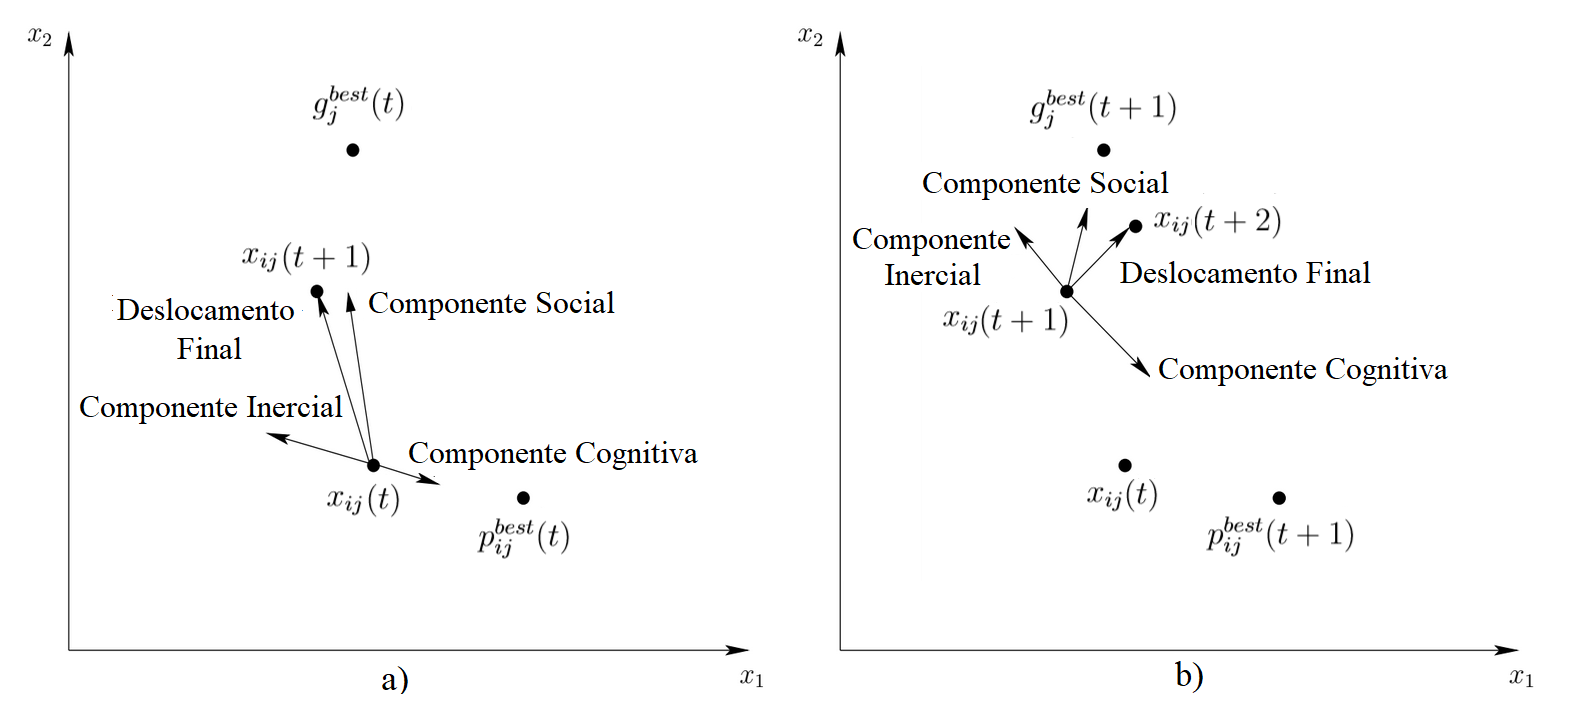
\includegraphics[width=160mm, height = 65mm]{images/pso_mov.png}
\fonte{Adaptado de \citeonline{compint}.}
\label{pso_mov}
\end{figure}



\SetKwFor{Enqto}{enquanto}{fa\c{c}a}{fim enqto}
\SetKwBlock{Inicio}{início}{fim}
\SetKwFor{ParaCada}{para cada}{fa\c{c}a}{fim para cada}
\SetKwIF{Se}{SenaoSe}{Senao}
{se}{então}{senão se}{senão}{fim se}
\SetKwInput{Saida}{Saída}


\begin{algorithm}[t]
\caption{\label{alg:pso} Algoritmo PSO}

\Entrada{número total de partículas ($n_p$), coeficientes de aceleração para as componentes cognitiva e social ($c_1$ e $c_2$), valores máximo e mínimo do peso de inércia ($w^{max}$ e $w^{min}$), número máximo de iterações ($k^{max}$), número de variáveis do problema ($m$), limites de velocidades máxima e mínima ($v^{max}_{ij}$ e $v^{min}_{ij}$).}

\Saida{Solução: $g^{best}_j(k)$.}

\Inicio{

Inicializar contador de iterações $k$=0. Inicializar aleatoriamente $n_p$ partículas que representam o enxame. Inicializar aleatoriamente $n_p$ velocidades iniciais. Inicializar todas as memórias das partículas como $p^{best}_{ij}(k)$ = $x_{ij}(k)$ e $g^{best}_{j}(k)$ como sendo a partícula com melhor avaliação da função objetivo de $p^{best}_{ij}(k)$. 

\Enqto{$t<t^{max}$}{
Atualizar peso de inércia utilizando a equação (\ref{peso});\\
\ParaCada{partícula $i = 1,...,n_p$}{
\Se{f($x_{ij}(k)$) < f($p^{best}_{ij}(k)$)}
{
// atualiza o $p^{best}_{ij}$ da partícula \\
$p^{best}_{ij}(k)$ = $x_{ij}(k)$;}

\Se{f($p^{best}_{ij}(k)$) < f($g^{best}_j(k)$)}
{
// atualiza o $g^{best}_j$ do enxame\\
$g^{best}_j(k)$ = $p^{best}_{ij}(k)$;}

Atualizar a velocidade da partícula utilizando a equação (\ref{pso_vel});\\
Limitar velocidades utilizando o procedimento (\ref{clampvel});\\
Atualizar a posição da partícula utilizando a equação (\ref{pso_posi});\\
}
$k=k+1$;
}
}

* $f(\cdot)$ representa a função objetivo de um problema de otimização irrestrito genérico.\\
\end{algorithm}


A metaheurística PSO, embora seja um dos algoritmos de maior destaque e aplicação na resolução de problemas relacionados ao FPO \cite{abbas, metareview}, possui como principal ponto negativo o problema de convergência precoce. \citeonline{maldicao2}, constataram que em problemas de grandes dimensões, metaheurísticas tendem a ter uma degradação em sua performance. \citeonline{maldicao}, concluíram o mesmo para as metaheurísticas PSO e ED, especificamente. O fenômeno ocorre devido ao fato de que o volume do hiperespaço de busca tende a crescer exponencialmente com o número de dimensões, tornando a cobertura efetuada pelas partículas esparsa e suscetível à convergência precoce para um mínimo local do problema. \citeonline{clpso}, também constataram o fenômeno de convergência precoce para problemas com função objetivo do tipo multimodal. Para aprimorar o desempenho do algoritmo em tais circunstâncias, propuseram uma nova variante denominada CLPSO que utiliza uma estratégia de aprendizagem abrangente para as partículas do enxame.


\subsection{Aprendizagem Abrangente}

Na metaheurística original de PSO, cada partícula aprende simultâneamente com $g^{best}_{j}(k)$ e $p^{best}_{ij}(k)$ a cada iteração. \citeonline{clpso} observaram que, em casos multimodais de grandes dimensões, a componente social apresenta um grande impacto no fenômeno de convergência prematura do algoritmo, pois as partículas do enxame tendem a convergir facilmente para a posição $g^{best}_{j}(k)$ mesmo que esta esteja distante da solução ótima global do problema de otimização. Se $p^{best}_{ij}(k)$ e $g^{best}_{j}(k)$ encontram-se em lados opostos de uma determinada partícula, esta tenderá a oscilar e eventualmente ser atraída para a posição $g^{best}_{j}(k)$, uma vez que a componente |$g^{best}_{j}(k)$-$x_{ij}(k)$| geralmente tende a ser maior que |$p^{best}_{ij}(k)$-$x_{ij}(k)$|. Por outro lado, se $p^{best}_{ij}(k)$ e $g^{best}_{j}(k)$ encontram-se na mesma região em relação a atual posição de uma determinada partícula, esta irá mover-se em direção a tal região e tenderá a ficar presa uma vez que $p^{best}_{ij}(k)$ e $g^{best}_{j}(k)$ encontram-se próximos, diminuindo a amplitude de movimento da partícula. Na estratégia de aprendizagem abrangente, as partículas aprendem utilizando informação da $p^{best}_{ij}(k)$ de outras partículas, tornando-as mais aptas a escaparem de possíveis mínimos locais do problema.

Na variante CLPSO, a atualização das posições das partículas é realizada utilizando-se a equação (\ref{pso_posi}). No entanto, a equação para o cálculo da velocidade é modificada para:

\begin{equation} \label{pso_vel2}
v_{ij}(k+1) = w(k) v_{ij}(k)+cr_{j}[mp^{best}_{ij}(k)-x_{ij}(k)],
\end{equation}

\noindent onde $c$ é constante e representa o novo coeficiente de aceleração, $r_{j}$ corresponde a um vetor de dimensão $m$ de números aleatórios provenientes de uma distribuição uniforme contínua $U(0,1)$ e $mp^{best}_{ij}(k)$ é um vetor de dimensão $m$ que corresponde à memória individual de cada partícula ($p^{best}_{ij}(k)$) modificada pela estratégia de aprendizagem abrangente. Comparando-se as equações de velocidade (\ref{pso_vel}) e (\ref{pso_vel2}) dos algoritmos PSO e CLPSO, respectivamente, pode-se notar:

\begin{itemize}
    \item No algoritmo CLPSO, a parcela da componente social é excluída da equação de atualização da velocidade, de forma que o deslocamento final deixa de depender de $g^{best}_{j}$;
    \item Modifica-se a componente cognitiva através da alteração da memória individual de cada partícula $p^{best}_{ij}$ para $mp^{best}_{ij}$. 
    
\end{itemize}

A estratégia de aprendizagem abrangente é aplicada para cada partícula do enxame, a cada iteração, conforme o intervalo de atualização (do inglês \emph{refreshing gap} ou $r^{gap}$) definido pelo usuário \cite{clpso}. Inicialmente, verifica-se a quantas iterações a partícula está sem obter progresso na otimização de sua função objetivo ($gap_i$). Caso o $gap_i$ da partícula $i$ seja maior ou igual a $r^{gap}$ definido pelo usuário, a partícula é então selecionada para passar pelo processo de aprendizagem abrangente e seu $gap_i$ é zerado. Em seguida, para cada uma das dimensões j = 1,...,m que compõem a partícula, sorteia-se um número aleatório proveniente de uma distribuição uniforme contínua $U(0,1)$ e verifica-se se este é inferior ou igual a uma probabilidade de troca ($p_t$) definida pelo usuário. Em caso negativo, a memória modificada da partícula receberá, nesta dimensão, o próprio valor de sua memória individual original $mp^{best}_{ij} = p^{best}_{ij}$. Caso o número sorteado seja inferior ou igual à $p_t$, duas outras memórias individuais das partículas do enxame são selecionadas aleatoriamente (excluindo-se deste sorteio a partícula que está sofrendo o processo de aprendizagem abrangente). Em seguida, verifica-se qual destas partículas sorteadas possui a melhor avaliação da função objetivo do problema (torneio). A partícula sob o processo de aprendizado irá, então, receber a informação da respectiva dimensão da memória individual da partícula vencedora do torneio $mp^{best}_{ij} = p^{best}_{vj}$, onde $p^{best}_{vj}$ denota o valor da dimensão $j$ da memória individual da partícula vencedora $v$. Uma vez executado este processo para todas as dimensões da partícula, verifica-se se a memória modificada resultante é igual a sua própria memória original. Caso seja, sorteia-se novamente outra memória individual dentre as partículas do enxame e uma dimensão, atribuindo-se, então, o novo valor à memória modificada. Este procedimento final garante que, ao final do processo de aprendizagem, a memória modificada da partícula nunca será totalmente equivalente a sua própria memória original.

Embora a parcela da componente social representada pela partícula $g^{best}_j$ tenha sido removida da equação da velocidade do algoritmo CLPSO, observa-se que o processo de aprendizagem abrangente permite com que a partícula possa aprender com as memórias individuais de outras partículas e a sua própria, preservando, portanto, os aspectos cognitivo e social do algoritmo PSO tradicional. Nesta nova variante, $p_t$ exerce um papel fundamental: quanto maior a probabilidade, mais as partículas aprendem com as memórias de outras partículas e, como consequência, aprimora-se a capacidade de busca global e diversificação do enxame. Por outro lado, quanto menor a probabilidade, menos informação é trocada pelas partículas, favorecendo o processo de busca local. O parâmetro $r^{gap}$, por sua vez, garante com que o processo de aprendizado ocorra apenas se a partícula esteja movimentando-se em direções pouco promissoras que não acarretem em melhoria do valor da função objetivo do problema em um determinado número de iterações. Desta forma, também evita-se com que boas direções sejam perdidas devido a um compartilhamento de informação excessivo. A formação de $mp^{best}_{ij}$ através da estratégia de aprendizagem abrangente pode ser sumarizada pelo algoritmo \ref{alg:cl}. Já a variante CLPSO está representada pelo algoritmo \ref{alg:clpso}.


\begin{algorithm}[!h]

\caption{\label{alg:cl} Estratégia de Aprendizagem Abrangente}

\Entrada{número total de partículas ($n_p$), probabilidade de troca ($p_t$), intervalo de atualização ($r^{gap}$), número de dimensões do problema ($m$), matriz de memórias individuais de cada partícula ($p^{best}_{ij}$), matriz de memórias individuais modificadas de cada partícula ($mp^{best}_{ij}$) e indicador de iterações sem aprimoramento da função objetivo de cada partícula ($gap_i$).}

\Saida {$mp^{best}_{ij}$ e $gap_i$.}

\Inicio{

\ParaCada{partícula $i = 1,...,n_p$}{

\Se{$gap_i >= r^{gap}$}{

\ParaCada{dimensão $j = 1,...,m$}{

\eSe{$(rand[U(0,1)] <= p_t)$}{
// sorteia aleatoriamente duas partículas de p^{best}_{ij} \\
$gap_i = 0$ \\
$a = \lceil{rand[U(0,1)]*n_p}\rceil$ \\
$b = \lceil{rand[U(0,1)]*n_p}\rceil$ \\

// executa torneio entre ambas as partículas sorteadas\\

\eSe{$f(p^{best}_{aj}) < f(p^{best}_{bj})$}
{
// salva valor da dimensão j da partícula com melhor avaliação \\

$mp^{best}_{ij} = p^{best}_{aj}$ \\
}
{
$mp^{best}_{ij} = p^{best}_{bj}$ \\
}
}
{
$mp^{best}_{ij} = p^{best}_{ij}$ \\
}

\Se{$mp^{best}_{ij} = p^{best}_{ij} \forall  j$}
{
$c = \lceil{rand[U(0,1)]*n_p}\rceil$ \\
$d = \lceil{rand[U(0,1)]*m}\rceil$ \\
$mp^{best}_{id} = p^{best}_{cd}$ \\
}
}
}
}
}
* $p^{best}_{aj}$ e $p^{best}_{bj}$ simbolizam, respectivamente, as memórias individuais da a-ésima e b-ésima partículas. $p^{best}_{cd}$ simboliza o valor da dimensão $d$ da memória individual da partícula $c$.

\end{algorithm}


\begin{algorithm}[htb]
\caption{\label{alg:clpso} Algoritmo CLPSO}
\Entrada{número total de partículas ($n_p$), coeficiente de aceleração($c$), valores máximo e mínimo do peso de inércia ($w^{max}$ e $w^{min}$), número máximo de iterações ($k^{max}$), número de variáveis do problema ($m$), probabilidade de troca ($p_t$) e intervalo de atualização ($r^{gap}$), limites de velocidades ($v^{max}_{ij}$ e $v^{min}_{ij}$).}\\
\Saida{Solução: $g^{best}_j(k)$.}


\Inicio{

Inicializar contador de iterações $t$=0. Inicializar aleatoriamente $n_p$ partículas que representam o enxame. Inicializar aleatoriamente $n_p$ velocidades iniciais. Inicializar todas as memórias das partículas como $p^{best}_{ij}(k)$ = $x_{ij}(k)$ e $g^{best}_{j}(k)$ como sendo a partícula com melhor avaliação da função objetivo de $p^{best}_{ij}(k)$. Inicializa o $gap_i$ de cada partícula como sendo nulo. Inicializa uma matriz $mp^{best}_{ij}(k)$ nula de mesmas dimensões que $p^{best}_{ij}(k)$. \\
\\

\Enqto{$t<t^{max}$}{
Atualizar peso de inércia utilizando a equação (\ref{peso});\\
\ParaCada{partícula $i = 1,...,n_p$}{
\Se{f($x_{ij}(k)$) < f($p^{best}_{ij}(k)$)}
{
$p^{best}_{ij}(k)$ = $x_{ij}(k)$;}
\Se{f($p^{best}_{ij}(k)$) < f($g^{best}_j(k)$)}
{
$g^{best}_j(k)$ = $p^{best}_{ij}(k)$;}

\eSe{f($x_{ij}(k)$) < f($x_{ij}(k-1)$)}
{
$gap_i=0$}{$gap_i=gap_i+1$}

Executar o procedimento de aprendizagem abrangente do algoritmo \ref{alg:cl};\\
Atualizar a velocidade da partícula utilizando a equação (\ref{pso_vel2});\\
Limitar velocidades conforme o procedimento (\ref{clampvel});\\
Atualizar a posição da partícula utilizando a equação (\ref{pso_posi});\\
}
$k=k+1$;
}
}

* $f(\cdot)$ representa a função objetivo de um problema de otimização genérico.\\
\end{algorithm}

No trabalho de \citeonline{clpso}, foram realizados testes computacionais em 16 diferentes funções para o algoritmo CLPSO, comparando-se os resultados com os de outras oito variantes da metaheurística PSO. Os autores concluíram que o algoritmo CLPSO melhora significativamente o desempenho da metaherística PSO e encontra os melhores resultados na maioria dos problemas multimodais quando comparados às demais variantes. Embora o desempenho não seja tão bom em problemas unimodais, os autores destacam que em aplicações do mundo real nem sempre se é possível conhecer as características do hiperespaço de soluções, sendo vantajoso, portanto, a utilização de algoritmos que desempenham bem em problemas multimodais. Os autores também aconselham a utilização de um método determinístico de otimização para aprimorar a capacidade do algoritmo em realizar buscas locais \cite{clpso_ls, clpso}, conceito que será utilizado neste trabalho. Na próxima seção, será apresentado o método desacoplado rápido utilizado para a resolução do FP.

\section{Método Desacoplado Rápido}

Nesta seção, foi adotada a mesma nomenclatura que a definida no Capítulo 2. O método FD, proposto por \citeonline{fdbx}, é um método eficaz e rápido para se obter a solução de problemas de FP. Trata-se de uma extensão do método de Newton-Raphson com certas aproximações que resultam em um algoritmo mais eficiente. Segundo \citeonline{monticelli1983fluxo}, este método explora o fato de que, em um sistema elétrico, as sensibilidades $\frac{\partial P}{\partial \theta}$ e $\frac{\partial Q}{\partial V}$ são mais intensas que as sensibilidades $\frac{\partial P}{\partial V}$ e $\frac{\partial Q}{\partial \theta}$. Em outras palavras, uma pequena mudança na magnitude da tensão de uma determinada barra não afeta o fluxo de potência ativa significativamente e, da mesma forma, uma pequena mudança no ângulo de fase da tensão de uma determinada barra pouco afeta o fluxo de potência reativa. Devido a essa interação física fraca entre tais variáveis, pode-se realizar o desacoplamento $P\theta$ - $QV$.

O desacoplamento permite um esquema de resolução no qual os subproblemas $P\theta$ e $QV$ são resolvidos alternadamente: na resolução do subproblema $P\theta$, são utilizados os valores atualizados de $V$. Já na resolução do subproblema $QV$, são utilizados os valores atualizados de $\theta$. Seja $g(x)$ formado pelos vetores $\Delta P$ e $\Delta Q$, que contêm as equações dos balanços de potência ativa (\ref{pot ativa}) e reativa (\ref{pot reativa}), respectivamente. O ponto central do processo de resolução de tal sistema ($g(x)=0$) pelo método de Newton-Raphson, é determinar o vetor de correção $\Delta x $ que resolve o sistema linear dado por:

\begin{equation} \label{newton}
g(x) = -J(x)\Delta x
\end{equation}

\noindent sendo $J$ a matriz jacobiana  de $g(x)$ e $x$ o vetor constituído pelas incógnitas $\theta$ e $V$. O sistema da equação (\ref{newton}) pode ser reescrito da seguinte maneira: 

\begin{equation} \label{newton2}
\begin{bmatrix}\Delta P\\ \Delta Q\end{bmatrix} = \begin{bmatrix}
H & N\\
M & L\\
\end{bmatrix} \begin{bmatrix} \Delta \theta\\ \Delta V
\end{bmatrix},
\end{equation}

\noindent onde $H=\frac{\partial P}{\partial \theta}$, $N=\frac{\partial P}{\partial V}$, $M=\frac{\partial Q}{\partial \theta}$ e $L=\frac{\partial Q}{\partial V}$. Já $\Delta \theta$ e $\Delta V$ são os vetores de correção dos ângulos e das magnitudes de tensão. Pela técnica de desacoplamento, as submatrizes M e N da matriz jacobiana são desconsideradas \cite{monticelli1983fluxo}, resultando em:

\begin{equation}\label{deltap}
\Delta P = H\Delta \theta,
\end{equation}
\begin{equation}\label{deltaq}
\Delta Q = L\Delta V,
\end{equation}

\noindent onde:

\begin{equation}\label{hk}
H = 
\begin{cases}
H_{km} =  \frac{\partial P_k}{\partial \theta_m} = V_{k}V_{m}\left[G_{km}\sin(\theta_{km}) - B_{km}\cos(\theta_{km})\right],\\

H_{kk} =  \frac{\partial P_k}{\partial \theta_k} = - B_{kk}V_k^2 - V_k\sum_{m \in \mathcal{B}} V_{m}\left[G_{km}\sin(\theta_{km}) - B_{km}\cos(\theta_{km})\right],
\end{cases}
\end{equation}

\begin{equation}\label{lk}
L = 
\begin{cases}
L_{km} =  \frac{\partial Q_k}{\partial V_m} = V_{k}\left[G_{km}\sin(\theta_{km}) - B_{km}\cos(\theta_{km})\right],\\
L_{kk} =  \frac{\partial Q_k}{\partial V_k} = - B_{kk}V_k - \sum_{m \in \mathcal{B}} {V_{m}\left[G_{km}\sin(\theta_{km}) - B_{km}\cos(\theta_{km})\right]}.
\end{cases}
\end{equation}



$G_{km}$ e $B_{km}$ são elementos das matrizes de condutância $G$ e susceptâncias $B$. Seja $V^{PQ}$ uma matriz diagonal cujos elementos não-nulos são as magnitudes de tensão nas barras de carga (PQ) do sistema. Pode-se redefinir as submatrizes jacobianas H e L como sendo: $H=V^{PQ}H'$ e $L=V^{PQ}L'$. As equações (\ref{deltap}) e (\ref{deltaq}) podem ser reescritas como:


\begin{equation}\label{deltap2}
\frac{\Delta P}{V^{PQ}} = H'\Delta \theta,
\end{equation}
\begin{equation}\label{deltaq2}
\frac{\Delta Q}{V^{PQ}} = L'\Delta V.
\end{equation}

Segundo \citeonline{fdbx}, na prática, as seguintes aproximações são quase sempre válidas para sistemas de transmissão:

\begin{itemize}
    \item $\theta_{km}$ é pequeno, de tal forma que $\cos(\theta_{km}) \approx 1$;
    \item $B_{km}$ é, em magnitude, muito maior que $G_{km}\sin{(\theta_{km})}$;
    \item $B_{kk}V_k^2$ é, em magnitude, muito maior que V_k\sum_{m \in \mathcal{B}} V_{m}\left[G_{km}\sin(\theta_{km}) - B_{km}\cos(\theta_{km})\right].
    
\end{itemize}

Desta forma, $H'$ e $L'$ podem ser reescritos como:

 
\begin{equation}\label{hk'}
H' = 
\begin{cases}
H'_{km} =  -V_{m}B_{km},\\

H_{kk} =  -B_{kk}V_k, \end{cases}
\end{equation}

\begin{equation}\label{lk'}
L = 
\begin{cases}
L_{km} = -B_{km},\\
L_{kk} =  -B_{kk}.
\end{cases}
\end{equation}

Considerando ainda que $V_k$ e $V_m$ são aproximadamente unitários: 

\begin{equation}\label{hk''}
H' = B',
\end{equation}

\begin{equation}\label{lk''}
L' = B".
\end{equation}

\noindent onde $B'$ e $B"$ são matrizes que dependem apenas dos parâmetros da rede, não dependendo, portanto, das incógnitas (ângulos e magnitudes das tensões nodais). Ambas as matrizes são semelhantes à matriz de susceptâncias $B$, no entanto, $B'$ não possui as linhas e colunas relacionadas às barras de referência ($V\theta$) e  $B"$ não possui as linhas e colunas relacionadas às barras ($V\theta$) e de geração ($PV$). Assim, são mantidas as estruturas das submatrizes jacobianas $H$ e $L$. Por dependerem apenas dos parâmetros da rede, $B'$ e $B"$ são constantes e precisam ser invertidas somente no início do processo. Por fim, as equações (\ref{deltap2}) e (\ref{deltaq2}) podem ser reescritas como:

\begin{equation}
\frac{\Delta P}{V^{PQ}} = B'\Delta \theta,
\end{equation}
\begin{equation}
\frac{\Delta Q}{V^{PQ}} = B"\Delta V.
\end{equation}

Na Figura \ref{fdflux}, pode-se observar o fluxograma do algoritmo FD. No fluxograma, KP e KQ são variáveis auxiliares que indicam a convergência (KP = 0 e KQ = 0) ou não (KP = 1 e KQ = 1) dos balanços de potência ativa e reativa nas barras do sistema, respectivamente. \citeonline{fdbx}, adotaram as equações (\ref{misp}) e (\ref{misq}) como critérios de convergência:

\begin{equation}\label{misp}
\lVert \Delta P \rVert_{\infty} \leq \tau_p,
\end{equation}
\begin{equation}\label{misq}
\lVert \Delta Q \rVert_{\infty} \leq \tau_q,
\end{equation}

\noindent onde, $\tau_p$ e $\tau_q$ são as tolerâncias definidas para o \emph{mismatch} dos balanços de potência ativa e reativa do sistema, respectivamente. 

Algumas melhorias no desempenho do método foram observadas quando, na formação da matriz $B'$, desprezaram-se as resistências série das linhas, aproximando-se as susceptâncias $b_{km}$ por $\frac{-1}{x_{km}}$, onde $x_{km}$ corresponde à reatância série da linha ou transformador que conecta as barras $k$ e $m$. Este método ficou conhecido como desacoplado rápido versão BX (do inglês \emph{fast-decoupled BX version} ou FDBX), sendo a versão mais utilizada para resolução do FP. As matrizes $B'$ e $B"$ podem ser representadas por:

\begin{equation}\label{b'}
B' = 
\begin{cases}
B'_{km} = -\frac{1}{x_{km}},\\

B'_{kk} =  \sum_{m \in \sigma_{k}}{\frac{1}{x_{km}}\right]. \end{cases}
\end{equation}

\begin{equation}\label{b''}
B" = 
\begin{cases}
B"_{km} =  - B_{km},\\

B"_{kk} =  - B_{kk}. \end{cases}
\end{equation}


\begin{figure}[!h]
\centering
\caption{Fluxograma do Algoritmo FD}
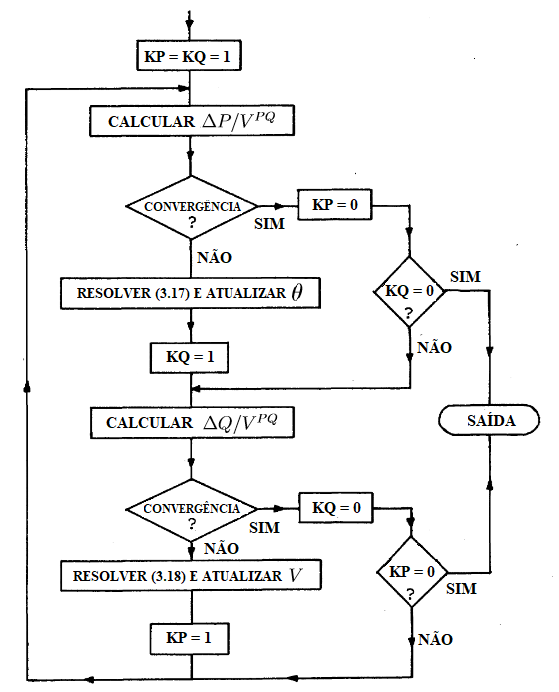
\includegraphics{images/fluxograma_fd.png}
\fonte{Adaptado de \citeonline{fdbx}.}
\label{fdflux}
\end{figure}

O método FD desempenha um papel importante no algoritmo híbrido desenvolvido neste trabalho, uma vez que diminui a quantidade de variáves a serem utilizadas durante a execução da metaheurística e ajuda a satisfazer as restrições de igualdade do problema. Isto permite uma atenuação do efeito da maldição da dimensionalidade e a diminuição da quantidade de penalizações a serem incorporadas na função objetivo do problema.

Na próxima seção, será apresentada a técnica BB utilizada para o tratamento das variáveis discretas dos problemas de FPO e FPOR.


\section{Método \emph{Branch-and-Bound}}

O método BB foi desenvolvido para solucionar problemas de programação inteira mista (PIM), sendo adaptado por \citeonline{bb} para problemas cujas funções são não lineares. O método, inicialmente, realiza a relaxação do problema com variáveis inteiras ou discretas e, então, divide-o em vários subproblemas até encontrar soluções que sejam factíveis. Seja um problema genérico de programação não linear e inteira mista (PNLIM), definido por (\ref{probgen}):

\begin{equation} \label{probgen}
\begin{aligned}
\text{min}  & \quad f(x,y) \\
\text{s.a:} &\quad   h(x,y) = 0 \\
&\quad   g(x,y) \leq 0 \\
&\quad x^{min}_i \leq x_i \leq x^{max}_i\\
&\quad y_i \in D_i,\quad i=1,...,n_y ,\\
\end{aligned}
\end{equation}

\noindent onde $x \in \mathbb{R}^{n_x}$, $y \in \mathbb{R}^{n_y}$, $f: \mathbb{R}^n \rightarrow \mathbb{R}$ e $h,g: \mathbb{R}^n \rightarrow \mathbb{R}^m$. Os limites superiores e inferiores das variáveis contínuas são representados por $x^{max}_i$ e $x^{min}_i$, enquanto que $D_i$ representa o conjunto com os valores inteiros permitidos da variável $y_i$. O problema representado por (\ref{probgen}) pode ser reescrito em sua forma relaxada como (\ref{probgenrelax}):

\begin{equation} \label{probgenrelax}
\begin{aligned}
\text{min}  & \quad f(x,y) \\
\text{s.a:} &\quad   h(x,y) = 0 \\
&\quad   g(x_i,y_i) \leq 0 \\
&\quad x^{min}_i \leq x_i \leq x^{max}_i,\quad i=1,...,n_x\\
&\quad y^{min}_i \leq y_i \leq y^{max}_i \quad i=1,...,n_y ,\\
\end{aligned}
\end{equation}

\noindent em que $y^{min}_i$ e $y^{max}_i$ denotam os valores mínimos e máximos do conjunto de valores inteiros $D_i$. Se ao resolver o problema relaxado (\ref{probgenrelax}) através de um método determinístico apropriado for encontrada uma solução inteira mista em que $y_i \in D_i$, então, tem-se a solução ótima do problema (\ref{probgen}). Caso contrário, onde $y_i \notin D_i$, uma variável de $y_i$ definida como $y^S$ cuja solução não é inteira é escolhida para sofrer a ação do processo de ramificação, que irá gerar os dois subproblemas (\ref{sub1}) e (\ref{sub2}). O subproblema (\ref{sub1}) apresenta a mesma formulação que (\ref{probgenrelax}) com a inserção de uma restrição de desigualdade $y^S \leq S^{inf}$. Já o subproblema (\ref{sub2}), apresenta a mesma formulação que (\ref{probgenrelax}) com a inserção de uma restrição $y^S \geq S^{sup}$. As costantes $S^{inf}$ e $S^{sup}$ representam os valores inteiros imediatamente inferior e superior ao valor contínuo $y^S$, que pertencem ao seu respectivo conjunto de valores inteiros $D^S$. 

\begin{equation} \label{sub1}
\begin{aligned}
\text{min}  & \quad f(x,y) \\
\text{s.a:} &\quad   h(x,y) = 0 \\
&\quad   g(x,y) \leq 0 \\
&\quad x^{min}_i \leq x_i \leq x^{max}_i,\quad i=1,...,n_x\\
&\quad y^{min}_i \leq y_i \leq y^{max}_i \quad i=1,...,n_y\\
&\quad y^S \leq S^{inf}\\
\end{aligned}
\end{equation}


\begin{equation} \label{sub2}
\begin{aligned}
\text{min}  & \quad f(x,y) \\
\text{s.a:} &\quad   h(x,y) = 0 \\
&\quad   g(x,y) \leq 0 \\
&\quad x^{min}_i \leq x_i \leq x^{max}_i,\quad i=1,...,n_x\\
&\quad y^{min}_i \leq y_i \leq y^{max}_i \quad i=1,...,n_y\\
&\quad y^S \geq S^{sup}\\
\end{aligned}
\end{equation}

Cada subproblema gerado durante o processo de otimização é representado como um ``nó$"$ da ``árvore$"$ do método BB. Se a solução de tal nó for inteira, então, o processo de ramificação (\emph{branch}) é paralizado nesta sub-região. Cada nó resolvido fornece a informação de um limitante (\emph{bound}), sendo que caso alguma sub-região apresente limitante inferior ao do nó com a melhor solução inteira encontrada até determinada iteração do algoritmo, seu processo de ramificação é paralizado. Caso contrário, o processo descrito anteriormente é repetido recursivamente \cite{teseEdilaine}. A Figura \ref{bb} ilustra um exemplo de ``árvore$"$ gerada pelo método BB:


\begin{figure}[!h]
\centering
\caption{Exemplo de uma ``árvore$"$ genérica gerada pelo método BB.}
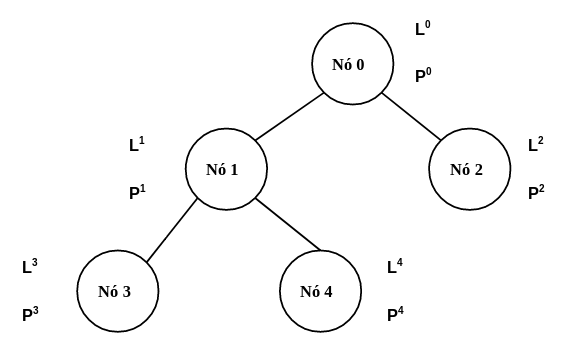
\includegraphics[width=100mm]{images/bbthree.png}
\fonte{Adaptado de \citeonline{arenales2015pesquisa}.}
\label{bb}
\end{figure}


Na Figura \ref{bb}, cada círculo representa um ``nó$"$ da ``árvore$"$. Cada ``nó$"$ $i$ representa um problema $P^{i}$ de otimização com valor de função objetivo (limitante) $L^i$. Segundo \citeonline{arenales2015pesquisa}, existem duas alternativas para a escolha do ``nó$"$ a ser explorado: a regra \emph{a priori} e a regra adaptativa. A regra \emph{a priori} mais utilizada é a busca em profundidade com \emph{backtracking}, onde o último ``nó$"$ incluído na lista é o primeiro a ser examinado. Na busca em profundidade, se um determinado ``nó$"$ não for eliminado, um de seus ``filhos$"$ será o próximo a ser examinado. O termo \emph{backtracking} implica que, quando um ``nó$"$ é eliminado, retorna-se em direção ao ``nó$"$ raíz até que se ache algum ``filho$"$ não explorado. A desvantagem desta técnica é a de que, pelo fato de não utilizar informação dos limitantes, acaba gerando ``árvores$"$ com um grande número de ``nós$"$. Já a regra adaptativa mais utilizada, é a de selecionar os ``nós$"$ a serem explorados com base nos valores de seus limitantes, explorando sempre aqueles que apresentam maior potêncial para a minimização da função objetivo do problema. Desta maneira, tem-se uma expectativa otimista em se encontrar uma nova solução factível com melhor valor da função objetivo em relação às soluções geradas pelos outros nós. A principal vantagem desta técnica é a utilização da informação do limitante,  que pode gerar ``árvores$"$ com um menor número de nós. Como desvantagem da regra adaptativa, pode-se citar a possibilidade de geração de muitos nós ativos e a consequente inviabilização da solução do problema devido ao limite de memória computacional.

Na próxima seção, será apresentado o método de programação quadrática sequencial utilizado para a execução da busca local no algoritmo híbrido.


\section{Método de Programação Quadrática Sequencial}

O método SQP foi elaborado no início da década de 1980, sendo o matemático M. J. D. Powell um de seus principais desenvolvedores \cite{sqp1,sqp2}. Trata-se de um algoritmo para problemas de otimização do tipo restritos, que converge para uma solução a medida que, simultâneamente, otimiza a função objetivo e melhora a factibilidade do problema. Seja um problema genérico de programação não linear (PNL):

\begin{equation} \label{pnl}
\begin{aligned}
\text{min}  & \quad f(x) \\
\text{s.a:} &\quad   h(x) = 0 \\
\end{aligned}
\end{equation}

\noindent onde \noindent onde $x \in \mathbb{R}^{n}$, $f: \mathbb{R}^n \rightarrow \mathbb{R}$ e $h: \mathbb{R}^n \rightarrow \mathbb{R}^m$. Para exemplificar o método SQP é necessário, inicialmente, começar pelas condições de Karush-Kuhn-Tucker (KKT) do problema (\ref{pnl}). A sua função lagrangiana $\mathcal{L}(x, \lambda)$ é dada pela equação:


\begin{equation} \label{lagrangiana}
\mathcal{L}(x, \lambda) = f(x) + h(x)}^\mathsf{T}\lambda,
\end{equation}

\noindent onde $\lambda \in \mathbb{R}^{m}$ representa os multiplicadores de Lagrange das restrições de igualdade. Derivando-se  a equação (\ref{lagrangiana}) em relação a $x$ e $\lambda$ e igualando-se as equações resultantes a zero, obtém-se as condições de KKT expressas por:

\begin{equation}
r =
\begin{bmatrix}
\nabla_x \mathcal{L}(x,\lambda) \\
\nabla_\lambda \mathcal{L}(x,\lambda) \\
\end{bmatrix}
=
\begin{bmatrix}
\nabla f(x) + J_h^\mathsf{T}\lambda\\
h(x)\\
\end{bmatrix}
= 0,
\end{equation}

\noindent onde $J_h^\mathsf{T} \in \mathbb{R}^{m \times n}$ representa a matriz jacobiana das restrições de igualdade do problema. Resolver o sistema de equações $r(u) = 0$ utilizando o método de Newton é o mesmo que resolver uma sequência de problemas lineares do tipo:

\begin{equation}
J_r(u_k)p_u = - r(u_k),
\end{equation}

\noindent em que $u \equiv \begin{bmatrix} x\\ \lambda \end{bmatrix}$, $J_r$ a jacobiana das derivadas $\frac{\partial r}{\partial u}$ e $p_u = u^{k+1}-u^k$.

Derivando-se o vetor de resíduos $r$ em relação aos vetores de variáveis concatenados em $u$, obtém-se o seguinte sistema de equações lineares:

\begin{equation}
\begin{bmatrix}\label{prim}
\mathcal{H_L} & J_h^\mathsf{T} \\
J_h & 0
\end{bmatrix}
\begin{bmatrix}
p_x \\
p_\lambda
\end{bmatrix}
= \begin{bmatrix}
- \nabla_x \mathcal{L} \\
- h
\end{bmatrix}.
\end{equation}

A cada iteração, as variáveis do problema e os multiplicadores de Lagrange são atualizados por:

\begin{equation}
x^{k+1} = x^k + p_x,
\end{equation}

\noindent e


\begin{equation}
\lambda^{k+1} = \lambda^k + p_\lambda,
\end{equation}

\noindent onde $p_x$ e $p_\lambda$ são os passos das variáveis $x$ e $\lambda$, respectivamente. Já $\mathcal{H_L}$ é a matriz hessiana da função lagrangiana. 

O método SQP pode ser derivado utilizando-se uma abordagem alternativa. Seja um problema de programação quadrática genérico expresso por (\ref{qp}):


\begin{equation} \label{qp}
\begin{aligned}
\text{min}  & \quad \frac{1}{2}x^\mathsf{T}Qx + q^\mathsf{T}x \\
\text{s.a:} &\quad   Ax+b=0\\
\end{aligned}
\end{equation}

\noindent em que $Q \in \mathbb{R}^{n \times n}$ e $q \in \mathbb{R}^n$ são, respectivamente, a matriz hessiana e o gradiente da função objetivo; $A \in \mathbb{R}^{m\times n}$  e $b \in \mathbb{R}^{m}$ são, respectivamente, a matriz de coeficientes e o vetor de termos independentes das restrições lineares. A função lagrangiana deste problema é definida por (\ref{lqp}):

\begin{equation} \label{lqp}
\mathcal{L}(x,\lambda) = \frac{1}{2}x^\mathsf{T}Qx + q^\mathsf{T}x + \lambda^\mathsf{T} [Ax+b].
\end{equation}

Portanto, o sistema formado pelas equações de KKT do problema (\ref{qp}) pode ser expresso por:

\begin{equation} \label{kktqp}
\begin{bmatrix}
Q & A^\mathsf{T}\\
A & 0 
\end{bmatrix}
\begin{bmatrix}
x\\
\lambda
\end{bmatrix}
=
\begin{bmatrix}
-q\\
-b
\end{bmatrix}
\end{equation}

As equações do sistema (\ref{kktqp}) são lineares e podem ser resolvidas diretamente. Para um problema genérico de PNL restrito, pode-se, portanto, realizar-se uma aproximação quadrática local e resolvê-lo sucessivamente até a sua convergência, o que representa a essência do método SQP. Realizando-se uma aproximação quadrática da lagrangiana (\ref{lagrangiana}) e uma aproximação linear das restrições de igualdade para um determinado passo $p_x$ em relação à variável $x$, obtém-se o seguinte problema do tipo quadrático:


\begin{equation} \label{qpap}
\begin{aligned}
\text{min}  & \quad \frac{1}{2}p_x^\mathsf{T}\mathcal{H_L}p_x + \nabla_xL^\mathsf{T}p_x \\
\text{s.a:} &\quad   J_hp_x+h=0\\
\end{aligned}
\end{equation}

\noindent o termo constante é desconsiderado uma vez que não modifica a solução. Substituindo-se $\nabla_xL^\mathsf{T}$ na função objetivo, obtém-se:

\begin{equation}
\frac{1}{2}p_x^\mathsf{T}\mathcal{H_L}p_x + \nabla_xf^\mathsf{T}p_x + \lambda^\mathsf{T}J_hp_x.
\end{equation}

Substituir $J_hp_x$ por $-h$, resulta em:

\begin{equation}
\frac{1}{2}p_x^\mathsf{T}\mathcal{H_L}p + \nabla_xf^\mathsf{T}p_x  -\lambda^\mathsf{T}h.
\end{equation}

Eliminando-se o termo $-\lambda^\mathsf{T}h$ por não depender de $p_x$, obtém-se o problema:

\begin{equation} \label{qpnl}
\begin{aligned}
\text{min}  & \quad \frac{1}{2}p_x^\mathsf{T}\mathcal{H_L}p + \nabla_xf^\mathsf{T}p_x \\
\text{s.a:} &\quad   J_hp_x + h =0\\
\end{aligned}
\end{equation}

A função lagrangiana do problema quadrático aproximado é dada por:

\begin{equation} \label{LL}
\mathcal{L}_{PQ}(p_x, \lambda) = \frac{1}{2}p_x^\mathsf{T}\mathcal{H_L}p_x + \nabla_xf^\mathsf{T}p_x + \lambda^{(k+1)}^\mathsf{T}[J_hp_x + h].
\end{equation}

Aplicando-se as condições de KKT, obtém-se o seguinte sistema de equações lineares:

\begin{equation} \label{sis}
\begin{bmatrix}
\mathcal{H_L} & J_h^\mathsf{T}\\
J_h^\mathsf{T} & 0
\end{bmatrix}
\begin{bmatrix}
p_x\\
\lambda^{k+1}
\end{bmatrix}
= 
\begin{bmatrix}
-\nabla_x f\\
-h
\end{bmatrix},
\end{equation}

\noindent onde $\lambda^{k+1}$ corresponde aos multiplicadores de Lagrange a serem utilizados na próxima iteração. Adotando-se que $\lambda^{k+1} = \lambda^k + p_\lambda$ e manipulando-se (\ref{sis}), encontra-se que:


\begin{equation} \label{sis2}
\begin{bmatrix}
\mathcal{H_L} & J_h^\mathsf{T}\\
J_h^\mathsf{T} & 0
\end{bmatrix}
\begin{bmatrix}
p_x\\
p_\lambda
\end{bmatrix}
=
\begin{bmatrix}
-\nabla_x f\\
-h
\end{bmatrix}
-
\begin{bmatrix}
J_h^\mathsf{T}\lambda^k\\
0
\end{bmatrix}
=\begin{bmatrix}
-\nabla_x \mathcal{L}\\
-h
\end{bmatrix}.
\end{equation}

Portanto, o sistema linear (\ref{sis2}) é equivalente ao sistema (\ref{prim}) encontrado a partir da aplicação direta do método de Newton nas condições de KKT do problema (\ref{pnl}).

O método SQP apresentado anteriormente também pode ser extendido para um problema genérico de PNL com $m_g$ restrições de desigualdade $g(x)$:

\begin{equation} \label{pnlg}
\begin{aligned}
\text{min}  & \quad f(x) \\
\text{s.a:} &\quad   h(x) = 0\\
&\quad   g(x) \leq 0, \\
\end{aligned}
\end{equation}

\noindent onde $g \in \mathbb{R}^n \rightarrow \mathbb{R}^d$. Neste caso, ao se realizar a aproximação quadrática e aplicar as condições de KKT ao problema (\ref{pnlg}), surge uma nova equação não linear que impede a resolução direta do método como visto anteriormente. Tal equação é decorrente da condição de folga complementar:

\begin{equation}
    \pi^\mathsf{T}(J_gp_x + g) = 0,
\end{equation}

\noindent onde $\pi \in \mathbb{R}^d$ e $J_g \in \mathbb{R}^{d\times n}$ correspondem, respectivamente, aos multiplicadores de Lagrange e à matriz jacobiana das restrições de desigualdade. Uma técnica comum para lidar com as restrições de desigualdade do problema (\ref{pnlg}) é a de conjuntos ativos (do inglês \emph{active set}). Seja a aproximação quadrática do problema (\ref{pnlg}) expressa por:

\begin{equation} \label{qpnlg}
\begin{aligned}
\text{min}  & \quad \frac{1}{2}p_x^\mathsf{T}\mathcal{H_L}p_x + \nabla_x\mathcal{L}^\mathsf{T}p_x \\
\text{s.a:} &\quad   J_hp_x + h =0\\
&\quad   J_gp_x + g \leq 0\\
\end{aligned}
\end{equation}

No início do algoritmo, verifica-se quais são as restrições de desigualdade que encontram-se ativas. O conjunto que possui as restrições ativas pode ser denotado por $\mathcal{A}^k$, para uma determinada iteração $k$ do algoritmo. Então, tais restrições são inseridas no problema como restrições de igualdade, eliminando-se a necessidade da condição de folga complementar. O problema (\ref{qpnlg}) pode ser reescrito por:

\begin{equation} \label{qpnlga}
\begin{aligned}
\text{min}  & \quad \frac{1}{2}p_x^\mathsf{T}\mathcal{H_L}p_x + \nabla_x\mathcal{L}^\mathsf{T}p_x \\
\text{s.a:} &\quad   J_hp_x + h =0\\
&\quad   J_{\sigma}p_x + \sigma = 0\\
\end{aligned}
\end{equation}

\noindent onde $\sigma$ e $J_\sigma$ são, respectivamente, os termos independentes e os coeficientes das restrições de desigualdade ativas, ou seja, restrições que pertencem ao conjunto $\mathcal{A}^k$. Conforme visto anteriormente, pode-se chegar ao seguinte sistema após manipular algebricamente a função objetivo e aplicar as condições necessárias de KKT:

\begin{equation} \label{sis20}
\begin{bmatrix}
\mathcal{H_L} & J_h^\mathsf{T} & J_\sigma^\mathsf{T}\\
J_h^\mathsf{T} & 0 & 0\\
J_\sigma^\mathsf{T} & 0 & 0
\end{bmatrix}
\begin{bmatrix}
p_x\\
p_\lambda\\
p_\pi
\end{bmatrix}
=\begin{bmatrix}
-\nabla_x \mathcal{L}\\
-h\\
-\sigma
\end{bmatrix},
\end{equation}

\noindent sendo que: $\pi^{k+1} = \pi^{k} + p_\pi$ e $\lambda^{k+1} = \lambda^{k} + p_\lambda$. Os multiplicadores de Lagrange das restrições de desigualdade ativas do problema são denotados por $\pi$. O sistema é resolvido encontrando-se os valores de $p_x$, $\lambda^{k+1}$ e $\pi^{k+1}$. Caso algum multiplicador de Lagrange $\pi^{k+1}$ seja negativo, a sua respectiva restrição de desigualdade deve ser retirada do conjunto ativo $\mathcal{A}^k$ e o seu valor definido como 0. 

Uma vez determinado $p_x$, calcula-se $x^{k+1} = x^k + p_x$ e executa-se um procedimento de busca em linha (do inglês \emph{line search}) de tal forma que uma função de mérito, estabelecida pela equação (\ref{merito}), apresente melhorias em relação à iteração anterior, ou seja $M(x^{k+1}, \lambda^{k+1},\pi^{k+1})<M(x^{k}, \lambda^{k},\pi^{k})$ \cite{sqpbook}}:

\begin{equation}\label{merito}
    M(x,\lambda,\pi) = f(x) + \lambda_v^\mathsf{T}\lVert h_v(x) \rVert + \pi_v^\mathsf{T}\lVert g_v(x) \rVert,
\end{equation}

\noindent onde: $h_v(x)$ e $g_v(x)$ representam as restrições do problema (\ref{pnlg}) que foram violadas. Já $\lambda_v$ e $\pi_v$ representam os multiplicadores de Lagrange das restrições violadas. Caso não haja melhorias na função mérito em relação à iteração anterior, deve-se determinar um novo $x^{k+1}$ tal que: $x^{k+1} = x^k + \alpha p_x$. Segundo \citeonline{sqpbook}, a escolha de $\alpha$ é geralmente arbitrária, sendo 0,5 um valor comum. Uma vez determinado $x^{k+1}$ que melhora a função de mérito, atualiza-se o conjunto de restrições ativas para a próxima iteração $\mathcal{A}^{k+1}$. Em seguida, para os novos valores de x, $\lambda$ e $\pi$, calcula-se: $\nabla f$, $J_g$, $J_h$ e $\nabla_x \mathcal{L}$. O algoritmo é executado até que $\lVert \nabla_x \mathcal{L}(x,\lambda,\pi) \rVert_\infty < \tau_{opt}$ ou $\lVert h(x) \rVert_\infty < \tau_{fact}$ e $\lVert g(x) \rVert_\infty < \tau_{fact}$, sendo $\tau_{fact}$ e $\tau_{tol}$ as tolerâncias de factibilidade das restrições e de otimalidade da função lagrangiana do problema (\ref{pnlg}), respectivamente \cite{sqpbook2}.

Conforme pode-se notar, o método SQP faz uso da informação de segunda ordem provinda da matriz hessiana da lagrangiana ($\mathcal{H_L}$) do problema (\ref{pnlg}) para determinar melhores direções de busca durante a execução do algoritmo. No entanto, o cálculo de tal matriz é computacionalmente dispendioso o que prejudica a eficiência do método. Para melhorar essa questão, na prática, são utilizados métodos do tipo Quase-Newton que aproximam a matriz hessiana com a informação de primeira ordem provinda do gradiente da lagrangiana ($\nabla_x \mathcal{L}$) a cada iteração. Assim, a matriz hessiana aproximada ($\mathcal{\tilde{H}_{L}}$) pode ser determinada pela técnica Broyden-Fletcher-Goldfarb-Shanno (BFGS):
\pagebreak
\begin{equation}\label{hessiana}
    \mathcal{\tilde{H}_{L}}^{k+1} = \mathcal{\tilde{H}_{L}}^{k}- \frac{\mathcal{\tilde{H}_{L}}^{k}\Delta x^k[\Delta x^k]^\mathsf{T}\mathcal{\tilde{H}_{L}}^{k}}{[\Delta x^k]^\mathsf{T}\mathcal{\tilde{H}_{L}}^{k}\Delta x^k} + \frac{y^{k}[y^{k}]^\mathsf{T}}{[\Delta x^k]^\mathsf{T}\Delta x^k},
\end{equation}

\noindent onde:

\begin{equation}
    \Delta x^k = x^{k+1} - x^{k},
\end{equation}

\noindent e

\begin{equation}
    y^k = \nabla_x\mathcal{L}(x^{k+1}, \lambda^{k+1}, \pi^{k+1})  - \nabla_x\mathcal{L}(x^{k}, \lambda^{k+1}, \pi^{k+1}).
\end{equation}

Na primeira iteração $k=0$, a matriz hessiana aproximada ($\mathcal{\tilde{H}_{L}}^{0}$)  é inicializada como uma matriz identidade ($I$). Segundo \citeonline{sqpbook2}, os multiplicadores de Lagrange estão fixados em seus valores mais recentes pois apenas é necessário aproximar a curvatura da lagrangiana no espaço das variáveis primais $x$. Vale ressaltar que, no método SQP, as soluções intermediárias obtidas satisfazem apenas as aproximações lineares dos subproblemas quadráticos. Com o decorrer das iterações, as aproximações tornam-se mais acuradas ao se aproximar da solução, satisfazendo, portanto, as restrições não lineares do problema original.

O método SQP juntamente com o MPI são considerados o estado da arte dos métodos determinísticos para a resolução de problemas de PNL restritos. Como vantagens do método SQP, pode-se citar: em contraste ao MPI, devido à estratégia de conjunto ativo, só é necessário considerar um subconjunto de restrições na resolução dos subproblemas, reduzindo-se, portanto, o tamanho destes. Além disso, segundo  \citeonline{sqpbook2} e \citeonline{apopt}, métodos SQP são mais adequados para a resolução de problemas utilizando-se a estratégia da boa-partida (do inglês \emph{warm-start}), princípio utilizado no algoritmo híbrido desenvolvido neste trabalho. Como desvantagem do método, pode-se citar: em contraste ao MPI, que apresenta um sistema de KKT fixo para todas as iterações, no método SQP, deve-se atualizar tal sistema caso o conjunto das restrições ativas seja modificado, o que pode exigir mais operações matemáticas e diminuir sua eficiência computacional. Por fim, pode-se sumarizar o método SQP através do algoritmo \ref{alg:sqp}. 

\begin{algorithm}[!h]
\caption{\label{alg:sqp} Algoritmo SQP}

\Entrada{ponto inicial ($x^0$), tolerância de otimalidade ($\tau_{opt}$) e tolerância de factibilidade ($\tau_{fact}$).}
\Saida{solução ótima local ($x^*$) e valor da função objetivo ($f(x^*)$).}


\Inicio{

Inicializar $k = 0$. Inicializar $\lambda^0 = 0$ e $\pi^0 = 0$. Determinar $f(x^0)$, $h(x^0)$ e $g(x^0)$. Determinar $J_g(x^0)$, $J_h(x^0)$ e $\nabla_x \mathcal{L}(x^0, \lambda^0, \pi^0)$. Determinar $\mathcal{A}^0$.\\

\Enqto{$(\lVert \nabla_x \mathcal{L}\rVert_\infty > \tau_{opt})$ ou $(\lVert h \rVert_\infty > \tau_{fact}$ e $\lVert g \rVert_\infty > \tau_{fact})$}{

\eSe{$k=0$}{$\mathcal{\tilde{H}_{L}}^{k} = I$}
{Calcular $\mathcal{\tilde{H}_{L}}^{k}$ pela equação (\ref{hessiana}).}\\

Determinar a aproximação quadrática (\ref{qpnlga}) do problema (\ref{pnlg}).\\
Aplicar as condições de KKT.\\
Resolver (\ref{sis2}). Determinar $p_x$, $p_\lambda$ e $p_\pi$.\\
Atualizar:\\
$\lambda^{k+1} = \lambda^{k} + p_\lambda$\\

$\pi^{k+1} = \pi^{k} + p_\pi$\\

$x^{k+1} = x^{k} + p_x$\\

\Se{$\pi^{k+1}<0$}
{ Redefinir $\pi^{k+1}=0$ e retirar a respectiva restrição do conjunto $\matehcal{A}^k$.}
Inicializar $\alpha = 1$.\\
\Enqto{$M(x^{k+1}, \lambda^{k+1}, \pi^{k+1})<M(x^{k}, \lambda^{k}, \pi^{k})$}
{// executa procedimento de busca em linha\\
$\alpha = \frac{\alpha}{2}$\\
$x^{k+1} = x^{k} + \alpha p_x$\\
}

Determinar $f(x^{k+1})$, $h(x^{k+1})$, $g(x^{k+1})$, $J_g(x^{k+1})$, $J_h(x^{k+1})$, $\nabla_x \mathcal{L}(x^{k+1}, \lambda^{k+1}, \pi^{k+1})$.\\
Atualizar $\mathcal{A}^{k+1}$.\\

$k=k+1$;
}
}
\end{algorithm}


Na próxima seção, serão apresentados as versões do método híbrido utilizadas na resolução dos problemas de DE com PCV, DE com PCV e ZOP, e FPOR.

\pagebreak
\section{Método Híbrido}

Nesta seção, serão apresentadas as versões do algoritmo híbrido utilizadas em cada um dos problemas abordados neste trabalho.

\subsection{Despacho Econômico com Ponto de Carregamento de Válvula}

O problema de DE (\ref{de_classic}) considerando os efeitos de PCV, é o mais simples dentre os problemas abordados neste trabalho. Por não considerar a RT, não é necessário utilizar o algoritmo FD para a resolução do FP. Além disso, por não possuir variáveis discretas, torna-se desnecessário utilizar o método BB. Portanto, na versão do algoritmo híbrido utilizada neste problema, são executados apenas a metaheurística CLPSO e o método SQP. No algoritmo CLPSO (\ref{alg:clpso}), para o problema de DE com PCV, cada partícula $x_{ij}(k)$ é representada por um vetor contendo as potências geradas por cada um dos $n$ geradores do sistema teste:

\begin{equation}
x_{ij}(k) = \begin{bmatrix}
P^G_1, & . & . & . &, P^G_n
\end{bmatrix}.
\end{equation}

As potências geradas para cada gerador $j$ são inicializadas, na primeira iteração, através da seguinte equação:

\begin{equation}\label{estrategia}
P^G_j = \underline{P^G_j} + [\overline{P^G_j}-\underline{P^G_j}]*rand()_j,
\end{equation}

\noindent onde $rand()_j$ simboliza um número aleatório proveniente de uma distribuição contínua uniforme $U(0,1)$. Tal inicialização garante com que todas as partículas sejam geradas aleatoriamente e as condições para os limites máximos e mínimos das potências estejam satisfeitas. As velocidades iniciais, que são vetores com as mesmas dimensões que as suas respectivas partículas, são inicializadas através da seguinte equação:

\begin{equation}\label{estrategia2}
v_{ij}(0) = \beta*rand()_j^{P},
\end{equation}

\noindent em que $rand()_j^{P}$ simboliza um número aleatório proveniente de uma distribuição uniforme contínua $U(-\overline{P^G_j},\overline{P^G_j})$, para cada gerador $j$. Já $\beta$ é uma constante de atenuação de valor pequeno. Após os cálculos de velocidades de cada partícula, a cada iteração, verifica-se se os limites máximos e mínimos estabelecidos foram violados conforme a equação (\ref{clampvel}). No método híbrido deste trabalho, utilizou-se como limitantes superiores $v^{max}_{ij}$ e inferiores $v^{min}_{ij}$ das velocidades, respectivamente:

\begin{equation}\label{vmax}
v^{max}_{ij} = \mu*[\overline{P^G_j}-\underline{P^G_j}]
\end{equation}

\noindent e

\begin{equation}\label{vmin}
v^{min}_{ij} = - \mu*[\overline{P^G_j}-\underline{P^G_j}],
\end{equation}

\noindent em que $\mu$ é um número pertencente ao intervalo [0,1] definido pelo usuário. A função \emph{fitness} $J(P^G_j)$, utilizada para avaliação das partículas neste problema, é composta pela função objetivo (\ref{custopcv}) e pela incorporação do método de penalização \cite{manual} por não satisfação da restrição da demanda de potência ativa do sistema, de forma a transformar um problema de otimização restrito em irrestrito:

\begin{equation}\label{fit}
J(P^G_j) = \sum_{j \in \mathcal{G}}{C_j(P^G_j)} + \Psi \lVert P^D - \sum_{j \in \mathcal{G}}{P^G_j}\rVert,
\end{equation}

\noindent onde $\Psi$ é uma constante que representa o fator de penalização da demanda. Quanto maior $\Psi$, maior a relevância da penalização na função \emph{fitness}. 

No decorrer do algoritmo, as partículas sobrevoam o hiperespaço de soluções procurando minimizar a equação (\ref{fit}). Durante a atualização de suas posições, é natural com que algum gerador tenha seu respectivo limite de potência violado. Neste caso, é executado um procedimento de restauração da potência do respectivo gerador cujo limite foi ultrapassado:


\begin{equation}\label{proc}
P^G_j = \begin{cases}
\underline{P^G_j}, \quad se & P^G_j < \underline{P^G_j}\\\\
\overline{P^G_j}, \quad se & P^G_j > \overline{P^G_j},\\\\
P^G_j, \quad se &\underline{P^G_j} \leq P^G_j \leq \overline{P^G_j}.
\end{cases}
\end{equation}


A condição (\ref{proc}) é executada para todas as potências de cada partícula em cada iteração do algoritmo, garantindo-se, portanto, que as partículas sempre estejam no interior da região factível do problema delimitada pelas restrições de desigualdade. Além disso, para facilitar com que nas iterações finais do método híbrido a geração de potência ativa da partícula $g^{best}$ satisfaça a restrição da demanda do sistema com uma determinada precisão $\tau_d$, foi desenvolvido o algoritmo \ref{alg:demanda} que é executado para toda iteração de valor superior a 80\% do número máximo de iterações. No algoritmo em questão, somam-se todas as potências de $g^{best}$ e verifica-se se o valor absoluto da diferença entre tal soma e a demanda total do sistema é inferior a uma precisão desejada. Caso não seja, divide-se tal diferença em $n$ parcelas iguais que são acrescentadas a cada gerador de $g^{best}$. Em seguida, corrige-se os geradores que eventualmente tenham seus limites violados conforme a condição (\ref{proc}). O procedimento em questão é repetido até que a precisão desejada seja encontrada.


Como visto na formulação matemática do problema de DE com PCV (\ref{de_classic}),  sua função objetivo é não diferenciável. No entanto, para a execução do método de otimização SQP, é necessária a informação proveniente do gradiente da função objetivo. Para tornar possível a aplicação do método neste problema, utilizou-se a mesma estratégia que a definida por \citeonline{pan2018hybrid}. Segundo os autores, pode-se obter um problema equivalente e diferenciável substituindo-se a parcela $|\sin(f_j[\underline{P^{G}_j}-P^{G}_j])|$ por variáveis auxiliares $s_j$, tal que:

\begin{equation}\label{de_aux}
\begin{aligned}
\text{min}  &\quad C_T(P^{G}) = \sum_{j \in \mathcal{G}} C_j(P^{G}_j) = \sum_{j \in \mathcal{G}} [a_j[P^{G}_j]^2 + b_jP^{G}_j + c_j + e_js_j]\\
\text{s.a:} &\quad \sum_{j \in \mathcal{G}}P^G_j = P^D \\
&\quad \underline{P^{G}_{j}} \leq P^{G}_{j} \leq \overline{P^{G}_{j}},\quad \forall j \in \mathcal{G}\\
&\quad s_j \geq \sin(f_j[\underline{P^{G}_j}-P^{G}_j]), \quad \forall j \in \mathcal{G}\\
&\quad s_j \geq -\sin(f_j[\underline{P^{G}_j}-P^{G}_j]), \quad \forall j \in \mathcal{G}.
\end{aligned}
\end{equation}


Desta maneira, o método determinístico pode ser aplicado ao problema (\ref{de_aux}) para aprimorar localmente a solução inicial fornecida pela metaheurística. O algoritmo \ref{alg:hibridode} resume o método híbrido proposto para resolução do problema de DE com PCV.


\begin{algorithm}[b!]
\caption{\label{alg:demanda} Algoritmo de ajuste da geração de potência ativa da partícula $g^{best}$.}

\Entrada{melhor partícula avaliada do enxame ($g^{best}$), demanda de potência ativa do sistema ($P^D$), valores máximos e mínimos dos limites de geração de potência ativa dos geradores ($\overline{P^{G}_j}$ e $\underline{P^{G}_j}$), número de geradores ($n$), precisão de atendimento da demanda ($\tau_{d}$), número máximo de iterações do algoritmo CLPSO ($k^{max}$), atual iteração do algoritmo CLPSO ($k$).}\\

\Saida{Solução: partícula $g^{best}$ ajustada.}


\Inicio{

\Se{$k>0,8*k^{max}$}{
\BlankLine
$dif = \sum_{j=1}^{n}[g^{best}_j] - P^D$
\BlankLine

\Enqto{$\lVert dif \rVert$ < $\tau_{d}$}{
\BlankLine
$val = dif/n$
\BlankLine
\ParaCada{gerador $j = 1,...,n$}{
\BlankLine
$g^{best}_j = g^{best}_j + val$\\
\BlankLine
\Se{$g^{best}_j < \underline{P^G_j}$}{
\BlankLine
\BlankLine
$g^{best}_j = \underline{P^G_j}$}
\BlankLine

\Se{$g^{best}_j > \overline{P^G_j}$}{
\BlankLine
\BlankLine
$g^{best}_j = \overline{P^G_j}$}
\BlankLine
}
\BlankLine
$dif = \sum_{j=1}^{n}[g^{best}_j] - P^D$

}
}
}

\end{algorithm}

\begin{algorithm}[hbt!]
\caption{\label{alg:hibridode} Algoritmo híbrido para o problema DE com PCV.}

\Entrada{número total de partículas ($n_p$), coeficiente de aceleração($c$), valores máximo e mínimo do peso de inércia ($w^{max}$ e $w^{min}$), número máximo de iterações ($k^{max}$), número de geradores do problema ($n$), probabilidade de troca ($p_t$), intervalo de atualização ($r^{gap}$), fator de penalização da demanda ($\Psi$), fator de limite de velocidade ($\mu$), precisão de atendimento da demanda $\tau_d$.}\\
\Saida{Solução: partícula $g^{best}$ aprimorada localmente pelo método SQP.}


\Inicio{

Carregar dados do caso teste. Inicializar contador de iterações $k$=0. Inicializar aleatoriamente $n_p$ partículas conforme (\ref{estrategia}) que representam o enxame. Inicializar aleatoriamente $n_p$ velocidades iniciais conforme (\ref{estrategia2}). Inicializar todas as memórias das partículas como $p^{best}_{ij}(k)$ = $x_{ij}(k)$ e $g^{best}_{j}(k)$ como sendo a partícula com melhor avaliação da função objetivo de $p^{best}_{ij}(k)$. Inicializa o $gap_i$ de cada partícula como sendo nulo. Inicializa uma matriz $mp^{best}_{ij}(k)$ nula de mesmas dimensões que $p^{best}_{ij}(k)$. \\
\\

\Enqto{$k<k^{max}$}{
Atualizar peso de inércia utilizando a equação (\ref{peso});\\
\ParaCada{partícula $i = 1,...,n_p$}{
\Se{J$(x_{ij}(k))$ < J$(p^{best}_{ij}(k))$}
{
$p^{best}_{ij}(k)$ = $x_{ij}(k)$;}
\Se{J$(p^{best}_{ij}(k))$ < J$(g^{best}_j(k))$}
{
$g^{best}_j(k)$ = $p^{best}_{ij}(k)$;}

\eSe{J$(x_{ij}(k))$ < J$(x_{ij}(k-1))$}
{$gap_i=0$}{$gap_i=gap_i+1$}
Executar o procedimento de aprendizagem abrangente do algoritmo \ref{alg:cl};\\
Atualizar a velocidade da partícula utilizando a equação (\ref{pso_vel2});\\
Limitar velocidade da partícula com base nas equações (\ref{clampvel}), (\ref{vmax}) e (\ref{vmin});\\
Atualizar a posição da partícula utilizando a equação (\ref{pso_posi});\\
Restaurar geradores com potências violadas utilizando o Procedimento (\ref{proc}).\\
Executa algoritmo \ref{alg:demanda} de ajuste da demanda para $g^{best}$;
}
$k=k+1$;
}
Reformular o problema DE com PCV para (\ref{de_aux}).\\ 
Executar o método SQP descrito pelo algoritmo \ref{alg:sqp}, sendo  $g^{best}_j$ o ponto inicial.
}

\end{algorithm}

Na versão do algoritmo híbrido proposto para este problema, a metaheurística CLPSO foi implementada em linguagem Python e o método SQP foi utilizado a partir do \emph{solver} APOPT disponível no pacote \emph{GEKKO Optimization Suite} para aplicações de otimização e aprendizado de máquina \cite{apopt}.

Na próxima seção, será apresentada a versão do método híbrido utilizada na resolução do problema de DE com PCV e ZOP.

\subsection{Despacho Econômico com Ponto de Carregamento de Válvula, Zonas de Operação Proibidas e Representação da Transmissão}

O problema de DE com PCV, ZOP e RT (\ref{PCV-ZOP-FPO}), impõe uma maior complexidade de resolução devido ao fato de ser não linear, multimodal, descontínuo e de grande dimensão. A presença da RT torna necessária a aplicação do método FD para resolução do FP. Já a presença de variáveis discretas e das ZOP torna necessário realizar adaptações na metaheurística CLPSO, bem como utilizar o método BB em conjunto com o método SQP.

Neste problema, cada partícula $x_{ij}(k)$ da metaheurística CLPSO é representada por um vetor contendo as variáveis independentes do SEP:


\begin{equation}
x_{ij}(k) = \begin{bmatrix}
V^G_1 . . . V^G_{n_v}, P^G_1 . . . P^G_{n_p}, t_1 . . . t_{n_t}, b^{sh}_1 . . . b^{sh}_{n_b}
\end{bmatrix},
\end{equation}

\noindent onde $V^G \in \mathcal{G}$ e $P^G \in \mathcal{G'}$ representam, respectivamente, os $n_v$ módulos de tensão e as $n_p$ potências ativas das barras de geração. Já $t \in \mathcal{T}$ e $b^{sh} \in \matehcal{B^{sh}}$ representam, respectivamente, os $n_t$ taps das linhas de transmissão e as $n_b$ susceptâncias \emph{shunt} dos bancos de capacitores e reatores \emph{shunt}. Cada variável $\mathcal{V}_j$ que constitui a partícula $x_{ij}(k)$ é inicializada conforme:

\begin{equation}\label{estrategia3} \mathcal{V}_j = \mathcal{V}_j^{min} + [\mathcal{V}_j^{max}-\mathcal{V}_j^{min}]*rand()_j,
\end{equation}

\noindent onde $\mathcal{V}_j^{min}}$ e $\mathcal{V}_j^{max}$ representam, respectivamente, os limitantes superiores e inferiores da variável $\mathcal{V}_j$. As velocidades iniciais são inicializadas conforme:


\begin{equation}\label{estrategia4}
v_{ij}(0) = \beta*rand()_j^{\mathcal{V}},
\end{equation}

\noindent em que $rand()_j^{\mathcal{V}}$ simboliza um número aleatório proveniente de uma distribuição uniforme contínua $U(-\mathcal{V}_j^{max},\mathcal{V}_j^{max})$. A cada iteração, as velocidades são limitadas pelos respectivos limites máximos e mínimos de velocidade de pela seguinte equação:


\begin{equation}\label{vmax1}
v^{max}_{ij} = \mu*[\mathcal{V}_j^{max}-\mathcal{V}_j^{min}]
\end{equation}

\noindent e

\begin{equation}\label{vmin1}
v^{min}_{ij} = - \mu*[\mathcal{V}_j^{max}-\mathcal{V}_j^{min}],
\end{equation}

Para cada partícula do método CLPSO, a cada iteração, é executado o método FD para satisfazer as restrições dos balanços de potência ativa e reativa do SEP, bem como determinar o valor das variáveis dependentes: ângulos $\theta \in \mathcal{B}$, módulos de tensão $V \in \mathcal{C}$, potências reativas geradas $Q^G \in \mathcal{G}$, bem como a potência ativa $P^G_{slack}$ gerada na barra de referência (do inglês \emph{slack}). A função de avaliação \emph{fitness}, portanto, é formada pelo custo, considerando os efeitos de PCV, somado às penalizações por ultrapassagem dos limitantes das variáveis dependentes:


\begin{equation}\label{fit2}
J(Q^G, P^G, V) = \sum_{a \in \mathcal{G}}{C_a(P^G_a)} + \zeta \sum_{b \in \mathcal{C}}{\lVert V_b - V^{lim}_b \rVert} + \omega \sum_{c \in \mathcal{G}}{\lVert Q^G_c - Q^{lim}_c \rVert} + \chi \lVert P^G_{slack} - P^{lim}_{slack} \rVert
\end{equation}

\noindent sendo que $\zeta$, $\omega$ e $\chi$ são constantes que representam, respectivamente, os fatores de penalização de ultrapassagem dos limites de tensão, potência reativa gerada pelos geradores e potência ativa gerada na barra \emph{slack}. Os valores de $V^{lim}b$, $Q^{lim}_c$ e $P^{lim}_{slack}$ podem ser definidos como:

\begin{equation}\label{proc1}
V^{lim}_b = \begin{cases}
\underline{V_b}, \quad se & V_b < \underline{V_b},\\\\
\overline{V_b}, \quad se & V_b > \overline{V_b},\\\\
V_b, \quad se & \underline{V_b} \leq V_b \leq \overline{V_b};
\end{cases}
\end{equation}


\begin{equation}\label{proc2}
Q^{lim}_c = \begin{cases}
\underline{Q^G_c}, \quad se & Q^G_c < \underline{Q^G_c},\\\\
\overline{Q^G_c}, \quad se & Q^G_c > \overline{Q^G_c},\\\\
Q^G_c, \quad se & \underline{Q^G_c} \leq Q^G_c \leq \overline{Q^G_c};
\end{cases}
\end{equation}


\begin{equation}\label{proc20}
P^{lim}_{slack} = \begin{cases}
\underline{P^G_{i}}, \quad se & P^{G}_{slack} < \underline{P^G_{i}},\\\\
\overline{P^G_{i}}, \quad se & P^{G}_{slack} > \overline{P^G_{i}},\\\\
P^G_{i}, \quad se & \underline{P^G_{i}} \leq P^G_{i} \leq \overline{P^G_{i}};
\end{cases}
\end{equation}

\pagebreak

\noindent em que $\overline{P^G_{i}}$ e $\underline{P^G_{i}}$ representam, respectivamente, os limitantes superiores e inferiores
da i-ésima zona de operação permitida mais próxima à atual posição da partícula para a variável dependente $P^G_{slack}$.

As restrições de desigualdade que retratam os limites superiores e inferiores das variáveis independentes $\mathcal{V}_j$, que constituem a partícula $x_{ij}(k)$, são tratadas pelo mesmo procedimento utilizado na versão do método híbrido para o problema de DE com PCV visto anteriormente:


\begin{equation}\label{proc10}
\mathcal{V}_j = \begin{cases}
\mathcal{V}_j^{min}, \quad se & \mathcal{V}_j < \mathcal{V}_j^{min},\\\\
\mathcal{V}_j^{max}, \quad se & \mathcal{V}_j > \mathcal{V}_j^{max},\\\\
\mathcal{V}_j, \quad se & \mathcal{V}_j^{min} \leq \mathcal{V}_j \leq \mathcal{V}_j^{max}.
\end{cases}
\end{equation}

Conforme visto na formulação matemática do problema (\ref{PCV-ZOP-FPO}), os taps dos transformadores e susceptâncias dos bancos de capacitores e reatores \emph{shunt} são variáveis discretas. Para lidar com tal restrição no algoritmo CLPSO, adotou-se uma estratégia similar à utilizada por \citeonline{psohibrido, antlion}. No trabalho destes autores, a cada iteração, as variáveis discretas das partículas eram arredondadas ao valor discreto mais próximo de seus respectivos conjuntos de valores discretos, o que acaba gerando um controle excessivo sobre o movimento das partículas, podendo causar a estagnação destas. No presente trabalho, optou-se por utilizar o mesmo procedimento de arredondamento, no entanto, apenas no momento da avaliação da partícula de tal forma que as variáveis independentes, no momento da resolução do FP e do cálculo da função \emph{fitness}, representam um cenário factível de operação para o problema. Ao terminar tal etapa de avaliação, as variáveis discretas que foram arredondadas são restauradas ao valor contínuo que possuiam previamente, de tal forma que, no decorrer das próximas etapas, a partícula irá continuar seu movimento partindo de sua posição original. A estratégia adotada evita com que ocorra uma estagnação do movimento das partículas devido ao arredondamento recorrente de suas variáveis discretas e, além disso, evita com que seja necessário utilizar mais penalizações na função \emph{fitness}. O procedimento de arredondamento pode ser definido como:

\begin{equation}\label{round}
    \mathcal{V}^d_j = round({V}^c_j),
\end{equation}

\pagebreak
\noindent onde $\mathcal{V}^c_j$ representa uma variável genérica de $x_{ij}(k)$ com valor contínuo que deve pertencer a um determinado conjunto discreto genérico $\mathcal{D}_j$. Já $\mathcal{V}^d_j$ representa a variável após o processo de arredondamento, enquanto que $round()$ representa o procedimento de arredondamento de $\mathcal{V}^c_j$ para o valor discreto de $\mathcal{D}_j$ mais próximo de seu atual valor contínuo.

De forma semelhante, as restrições de ZOP das potências ativas geradas pelos geradores podem ser satisfeitas aplicando-se um operador de modificação dos valores de $P^G$ infactíveis antes da resolução do FP e do cálculo do \emph{fitness}. Ao terminar tal etapa, as potências modificadas podem ser restauradas aos seus respectivos valores originais dando continuidade ao movimento natural da partícula. O procedimento pode ser definido como:


\begin{equation}\label{proc100}
P^G_j = \begin{cases}
\underline{P^G_{j,i}}, \quad se & P^G_j < \underline{P^G_{j,i}},\\\\
\overline{P^G_{j,i}}, \quad se & P^G_j > \overline{P^G_{j,i}},\\\\
P^G_{j}, \quad se & \underline{P^G_{j,i}} \leq P^G_j \leq \overline{P^G_{j,i}},
\end{cases}
\end{equation}

\noindent onde $\overline{P^G_{j,i}}$ e $\underline{P^G_{j,i}}$ representam, respectivamente, os limitantes superiores e inferiores de potência ativa $P^G$ do gerador $j$ na i-ésima zona de operação permitida mais próxima da atual posição da partícula.

Devido ao fato da função objetivo ser não diferenciável, também torna-se necessário reformular o problema (\ref{PCV-ZOP-FPO}) utilizando a estratégia de \citeonline{pan2018hybrid} para a aplicação do método SQP. Uma vez que o método determinístico é utilizado para aperfeiçoar localmente a solução fornecida pelo algoritmo CLPSO, adotam-se os limites da i-ésima zona de operação permitida onde a partícula $g^{best}$ se encontra como sendo os limites inferiores $\underline{P^{G}_{j,i}}$ e superiores $\overline{P^{G}_{j,i}}$ das potências ativas dos geradores do sistema, de modo a excluir as demais zonas do problema. 

Para as variáveis discretas $t$ e $b^{sh}$, restringem-se os seus respectivos conjuntos de valores discretos para os $n_d$ vizinhos imediatamente inferiores e superiores possíveis de cada \emph{tap} e susceptância \emph{shunt}, utilizando-se os valores encontrados na solução $g^{best}$ como sendo os valores centrais de referência dos novos conjuntos $C_{jm}^{tap}$ e $C_{jm}^{sh}$. Ambas as medidas citadas anteriormente diminuem consideravelmente o número de variáveis discretas para o método BB e, consequentemente, diminuem também o número de ``nós$"$ a serem explorados na árvore gerada durante a execução do método. Então, o problema (\ref{PCV-ZOP-FPO}) é reformulado para:


\begin{equation} \label{PCV-ZOP-FPO-2}
\begin{aligned}
\text{min}  &\quad C_T(P^{G}) = \sum_{j \in \mathcal{G}} C_j(P^{G}_j) = \sum_{j \in \mathcal{G}} [a_j[P^{G}_j]^2 + b_jP^{G}_j + c_j + e_js_j]\\
\text{s.a:} &\quad   \Delta P_j(V,\theta,t) = 0, \quad \forall j \in \mathcal{G}' \cup \mathcal{C} \\
&\quad   \Delta Q_j(V,\theta,t, b^{sh}) = 0, \quad \forall j \in \mathcal{C} \quad\\
&\quad \underline{P^{G}_{j,i}} \leq P^{G}_{j,i} \leq \overline{P^{G}_{j,i}},\quad \forall j \in \mathcal{G}\\
&\quad \underline{Q^{G}_{j}} \leq Q_{j}(V,\theta,t,b^{sh}) \leq \overline{Q^{G}_{j}}, \quad  \forall j \in \mathcal{G}\\
&\quad \underline{V_{j}} \leq V_{j} \leq \overline{V_{j}}, \quad  \forall j \in \mathcal{B}\\
&\quad b^{sh}_{j} \in C_{j}^{sh}, \quad \forall j \in \mathcal{B}^{sh}\\
&\quad t_{jm} \in C_{jm}^{tap},\quad \forall j,m \in \mathcal{T} \\
&\quad s_j \geq \sin(f_j[\underline{P^{G}_j}-P^{G}_j]), \quad \forall j \in \mathcal{G}\\
&\quad s_j \geq -\sin(f_j[\underline{P^{G}_j}-P^{G}_j]), \quad \forall j \in \mathcal{G}.\\
\end{aligned}
\end{equation}

Na versão do algoritmo híbrido \ref{alg:fpo} proposto para este problema , a metaheurística CLPSO foi implementada em linguagem Python; os dados do sistema elétrico e o método FD foram utilizados a partir do pacote \emph{pandapower} para simulações e análises de sistemas elétricos \cite{pp}; e o método SQP em conjunto com o método BB foram utilizados a partir do \emph{solver} APOPT disponível no pacote \emph{GEKKO Optimization Suite} \cite{apopt}.

\begin{algorithm}[hbt!]
\caption{\label{alg:fpo} Algoritmo Híbrido para o problema DE com PCV, ZOP e RT.}

\Entrada{número total de partículas ($n_p$), coeficiente de aceleração ($c$), valores máximo e mínimo do peso de inércia ($w^{max}$ e $w^{min}$), número máximo de iterações ($k^{max}$), probabilidade de troca ($p_t$), intervalo de atualização ($r^{gap}$) e fatores de penalização de: tensão ($\zeta$), potência reativa gerada ($\omega$) e potência ativa gerada na barra slack ($\chi$).}
\Saida{Solução: partícula $g^{best}_j$ aprimorada localmente pelo método SQP.}


\Inicio{

Inicializar contador de iterações $k$=0. Inicializar aleatoriamente $n_p$ partículas conforme (\ref{estrategia3}) que representam o enxame. Inicializar aleatoriamente $n_p$ velocidades iniciais conforme (\ref{estrategia4}). Inicializar todas as memórias das partículas como $p^{best}_{ij}(k)$ = $x_{ij}(k)$ e $g^{best}_{j}(k)$ como sendo a partícula com melhor avaliação da função objetivo de $p^{best}_{ij}(k)$. Inicializa o $gap_i$ de cada partícula como sendo nulo. Inicializa $mp^{best}_{ij}(k)$ nula de mesmas dimensões que $p^{best}_{ij}(k)$. \\
\\

\Enqto{$k<k^{max}$}{
Atualizar peso de inércia utilizando a equação (\ref{peso});\\
\ParaCada{partícula $i = 1,...,n_p$}{
Executa o procedimento de arredondamento: $x_{ij}^d(k) = round(x_{ij}(k))$. \\
Executa procedimento de ajuste das potências ativas (\ref{proc100}).\\
Executa o algoritmo FD \ref{fdflux} para resolução do FP.\\
\Se{J$(x_{ij}^d(k))$ < J$(p^{best}_{ij}(k))$}
{
$p^{best}_{ij}(k)$ = $x_{ij}(k)$;}
\Se{J$(x_{ij}^d(k))$ < J$(g^{best}_j(k))$}
{
$g^{best}_j(k)$ = $x_{ij}^d(k)$;}

\eSe{J$(x_{ij}^d(k))$ < J$(x_{ij}^d(k-1))$}
{$gap_i=0$}{$gap_i=gap_i+1$}
Executar o procedimento de aprendizagem abrangente do algoritmo \ref{alg:cl};\\
Atualizar a velocidade da partícula utilizando a equação (\ref{pso_vel2});\\
Limitar velocidades das partículas utilizando as equações (\ref{vmax1}) e (\ref{vmin1});\\
Atualizar a posição da partícula utilizando a equação (\ref{pso_posi});\\
Restaurar variáveis com limites violados utilizando o procedimento (\ref{proc10}).\\
}
$k=k+1$;
}
Reformular o problema DE com PCV, ZOP e RT para (\ref{PCV-ZOP-FPO-2}).\\ 
Executar o método BB com o algoritmo SQP \ref{alg:sqp}, sendo  $g^{best}_j$ o ponto inicial.
}

\end{algorithm}
Na próxima seção, será apresentada a versão do método híbrido utilizada na resolução do problema FPOR.
\pagebreak
\subsection{Fluxo de Potência Ótimo Reativo}

No problema de FPOR (\ref{FPOR}), ao contrário do problema de DE com PCV, ZOP e RT, as potências ativas geradas pelos geradores são tratadas como parâmetros do sistema e não mais como variáveis. Neste tipo de problema, preocupa-se em otimizar as variáveis que estão relacionadas ao fluxo de potência reativa no sistema, visando minimizar as perdas de energia nas linhas de transmissão. Da mesma forma que no problema da seção anterior, são consideradas a RT e as variáveis discretas dos \emph{taps} e susceptâncias dos bancos de capacitores e reatores \emph{shunt}. Portanto, as variáveis independentes que constituem uma determinada partícula $x_{ij}(k)$ são:

\begin{equation}\label{partfpor}
x_{ij}(k) = \begin{bmatrix}
V^G_1 . . . V^G_{n_v}, t_1 . . . t_{n_t}, b^{sh}_1 . . . b^{sh}_{n_b}
\end{bmatrix}.
\end{equation}

A inicialização das posições das partículas e de suas velocidades iniciais é feita, respectivamente, utilizando as equações (\ref{estrategia3}) e (\ref{estrategia4}). Para cada partícula do algoritmo CLPSO, a cada iteração, é executado o método FD para satisfazer as restrições dos balanços de potência ativa e reativa do SEP, bem como determinar o valor das variáveis dependentes. A função \emph{fitness} de avaliação das partículas, neste caso, é formada pelo somatório das perdas em cada ramo do sistema e por eventuais penalizações por ultrapassagem dos limites de tensão das barras PQ, geração de potência reativa nas barras PV e \emph{slack}, e potência ativa na barra \emph{slack}:

\begin{equation}\label{fit3}
J(Q^G, V, \theta, t) = P_L(V, \theta, t) + \zeta \sum_{b \in \mathcal{C}}{\lVert V_b - V^{lim}_b \rVert} + \omega \sum_{c \in \mathcal{G}}{\lVert Q^G_c - Q^{lim}_c \rVert},
\end{equation}

\noindent onde $V^{lim}_b$ e $Q^{lim}_c$ são definidos através das equações (\ref{proc1}) e (\ref{proc2}), respectivamente. Já as restrições de desigualdade das variáveis que constituem as partículas são tratadas no próprio algoritmo CLPSO através da equação (\ref{proc10}), a cada iteração.

Para lidar com as variáveis discretas $t$ e $b^{sh}$, utilizou-se a mesma estratégia de arredondamento definida pela equação (\ref{round}), onde as variáveis são arredondadas apenas na etapa de resolução do FP e avaliação, sendo reconstituídas ao seu valor contínuo logo após este processo, evitando a possibilidade de estagnação da partícula. Uma vez determinada a solução $g^{best}$ ao fim da execução da metaheurística CLPSO, restringem-se os conjuntos $\mathcal{D}^{tap}_{jm$ e $\mathcal{D}^{sh}_{j}$ de variáveis discretas para os $n_d$ vizinhos imediatamente superiores e inferiores possíveis de cada \emph{tap} e susceptância \emph{shunt},  dando origem aos novos conjuntos discretos $C^{tap}_{jm}$
 e $C^{sh}_{j}$. Como a função objetivo $P_L$ do problema de FPOR em sua versão relaxada é diferenciável e não envolve os efeitos de PCV, não é necessário utilizar a estratégia de \citeonline{pan2018hybrid}. O problema de FPOR, portanto, deve ser reformulado matematicamente para (\ref{FPOR2}) a fim de se executar a busca local utilizando-se os método BB e SQP:


\begin{equation} \label{FPOR2}
\begin{aligned}
\text{min}  &\quad P_L(V,\theta,t)  \\
\text{s.a:} &\quad   \Delta P_j(V,\theta,t) = 0, \quad \forall j \in \mathcal{G}' \cup \mathcal{C} \\
&\quad   \Delta Q_j(V,\theta,t, b^{sh}) = 0, \quad \forall j \in \mathcal{C} \quad\\
&\quad \underline{Q^{G}_{j}} \leq Q_{j}(V,\theta,t,b^{sh}) \leq \overline{Q^{G}_{j}}, \quad  \forall j \in \mathcal{G}\\
&\quad \underline{V_{j}} \leq V_{j} \leq \overline{V_{j}}, \quad  \forall j \in \mathcal{B}\\
&\quad b^{sh}_{j} \in C_{j}^{sh}, \quad \forall j \in \mathcal{B}^{sh}\\
&\quad t_{jm} \in C_{jm}^{tap},\quad \forall j,m \in \mathcal{T} \\
\end{aligned}
\end{equation}

\begin{algorithm}[hbt!]
\caption{\label{alg:fpor} Algoritmo Híbrido para o problema FPOR.}

\Entrada{número total de partículas ($n_p$), coeficiente de aceleração ($c$), valores máximo e mínimo do peso de inércia ($w^{max}$ e $w^{min}$), número máximo de iterações ($k^{max}$), probabilidade de troca ($p_t$), intervalo de atualização ($r^{gap}$) e fatores de penalização de: tensão ($\zeta$), potência reativa gerada ($\omega$) e potência ativa gerada na barra slack ($\chi$).}
\Saida{Solução: partícula $g^{best}_j$ aprimorada localmente pelo método SQP.}


\Inicio{

Inicializar contador de iterações $k$=0. Inicializar aleatoriamente $n_p$ partículas conforme (\ref{partfpor}) que representam o enxame. Inicializar aleatoriamente $n_p$ velocidades iniciais conforme (\ref{estrategia4}). Inicializar todas as memórias das partículas como $p^{best}_{ij}(k)$ = $x_{ij}(k)$ e $g^{best}_{j}(k)$ como sendo a partícula com melhor avaliação da função objetivo de $p^{best}_{ij}(k)$. Inicializa o $gap_i$ de cada partícula como sendo nulo. Inicializa $mp^{best}_{ij}(k)$ nula de mesmas dimensões que $p^{best}_{ij}(k)$. \\
\\

\Enqto{$k<k^{max}$}{
Atualizar peso de inércia utilizando a equação (\ref{peso});\\
\ParaCada{partícula $i = 1,...,n_p$}{
Executa o procedimento de arredondamento: $x_{ij}^d(k) = round(x_{ij}(k))$. \\
Executa o algoritmo FD \ref{fdflux} para resolução do FP.\\
\Se{J$(x_{ij}^d(k))$ < J$(p^{best}_{ij}(k))$}
{
$p^{best}_{ij}(k)$ = $x_{ij}(k)$;}
\Se{J$(x_{ij}^d(k))$ < J$(g^{best}_j(k))$}
{
$g^{best}_j(k)$ = $x_{ij}^d(k)$;}

\eSe{J$(x_{ij}^d(k))$ < J$(x_{ij}^d(k-1))$}
{$gap_i=0$}{$gap_i=gap_i+1$}
Executar o procedimento de aprendizagem abrangente do algoritmo \ref{alg:cl};\\
Atualizar a velocidade da partícula utilizando a equação (\ref{pso_vel2});\\
Limitar as velocidades das partículas conforme equações (\ref{vmax1}) e (\ref{vmin1});\\
Atualizar a posição da partícula utilizando a equação (\ref{pso_posi});\\
Restaurar variáveis com limites violados utilizando o procedimento (\ref{proc10}).\\
}
$k=k+1$;
}
Reformular o problema DE com PCV, ZOP e RT para (\ref{FPOR2}).\\ 
Executar o método BB com o algoritmo SQP \ref{alg:sqp}, sendo  $g^{best}_j$ o ponto inicial.
}

\end{algorithm}

Na versão do algoritmo híbrido proposto para este problema (\ref{alg:fpor}), a metaheurística CLPSO foi implementada em linguagem Python; os dados do sistema elétrico e o método FD foram utilizados a partir do pacote \emph{pandapower} \cite{pp}; e o método SQP em conjunto com o método BB foram utilizados a partir do \emph{solver} APOPT disponível no pacote \emph{GEKKO Optimization Suite}
\cite{apopt}.

No próximo capítulo serão apresentados os resultados dos testes numéricos realizados com os algoritmos híbridos desenvolvidos para os problemas de: DE com PCV; DE com PCV, ZOP e RT; e FPOR.


\chapter{Testes Numéricos}

Neste capítulo, serão apresentados os resultados obtidos pelos métodos híbridos desenvolvidos para os problemas abordados neste trabalho. Para avaliar o desempenho do algoritmo híbrido, serão realizadas comparações com outros métodos encontrados na literatura, metaheurísticas e \emph{solvers} de otimização. Todos os testes foram realizados em um computador com processador Intel® Core™ i5-8250U de 1,60 GHz com 8 GB de memória RAM.

\section{Despacho Econômico com Ponto de Carregamento de Válvula}

No Apêndice A, são apresentados os dados dos sistemas para os casos testes de 13, 19 e 40 unidades geradoras, bem como os dados dos testes realizados para determinar os hiperparâmetros do método híbrido. Para os casos testes do problema DE com PCV, utilizou-se as tolerâncias $\tau_d = 10^{-3}$ para o método CLPSO, e $\tau_{opt} = 10^{-3}$ com $\tau_{fact} = 10^{-3}$ para o método SQP.

\subsection{Caso 1: 13 Unidades Geradoras}

 Para o caso teste com 13 unidades geradoras, foi considerada uma demanda de 2520 MW. Os dados extraídos de \citeonline{dados13} dos limites de geração e dos coeficientes da função custo de cada gerador podem ser visualizados na Tabela \ref{13coef}. Além do método híbrido, foram também implementados, para fins de comparação, os otimizadores PSO, SQP (\emph{solver} APOPT) e CLPSO. Foram realizadas 50 execuções para a coleta de dados, sendo que para o método determinístico SQP foram utilizados 50 pontos iniciais aleatoriamente criados. Além disso, para tratar a não diferenciabilidade da função objetivo no método SQP, também adotou-se a técnica proposta por \citeonline{pan2018hybrid}. A formulação matemática e os dados utilizados neste trabalho coincidem com os utilizados nos trabalhos de: \citeonline{PSO-SQP} (PSO-SQP e EP-SQP), \citeonline{POTHIYA2010478} (ACO), \citeonline{dissertacaodiego} (PDPCBLM) e \citeonline{dissertacaojv} (ED e ED-BFGS). 
 
 A Tabela \ref{config13} mostra as configurações de hiperparâmetros utilizados nos métodos PSO e CLPSO, sendo que as colunas não preenchidas simbolizam parâmetros que não existem na metaheurística em questão. Para a metaheurística PSO, adotaram-se valores comumente vistos na literatura \cite{psohibrido, pso_artigo}. Em ambos os casos foi utilizado um peso de inércia linearmente decrescente. O critério de parada para as metaheurísticas foi de 1000 iterações, com enxames de 75 partículas.
 
 
\begin{table}[h!]
\centering
\caption{\label{config13} Hiperparâmetros das metaheurísticas PSO e CLPSO.}

\begin{tabular}{c c c c c c c c c c c }
	\hline
    Método & $c_1$ & $c_2$ & $c$ & $w^{min}$ & $w^{max}$ & $r^{gap}$ & $p_t$ &  \beta & $\Psi$ & $\mu$ \\
    
    PSO & 2 & 2 & - & 0,4 & 0,9 & - & - &  0,1 & 10 & 0,25 \\
    
    CLPSO & - & - & 1 & 0,4  & 0,9 & 0 & 0,4 &  0,1 & 10 & 0,25 \\    
    
    \hline
\end{tabular}
\fonte{Autor.}
\end{table}
 
 A Tabela \ref{resultados13} traz os valores obtidos de custo mínimo, custo médio e desvio padrão para cada método utilizado na comparação. Alguns autores reportaram apenas dados a respeito do custo mínimo obtido, não utilizando as métricas de custo médio e desvio padrão. Os trabalhos de \citeonline{dissertacaodiego} e \citeonline{POTHIYA2010478} trazem valores de custos que não condizem com os valores calculados a partir de suas soluções informadas.


\begin{table}[h!]
\centering
\caption{\label{resultados13}Valores mínimos, médios e desvios padrão obtidos para a função custo do problema de DE com PCV no caso 1.}

\begin{tabular}{c c c c}
	\hline
	\textbf{\makecell{Método}} & \textbf{\makecell{Custo\\Mínimo (\$)}} &
	\textbf{\makecell{Custo\\Médio (\$)}} & \textbf{\makecell{Desvio\\Padrão (\$)}}\\ 
	\hline
	
	
	\makecell{PSO} &  \makecell{24327,0992}   & \makecell{24682,0751}  &  187,9927  \\

	\makecell{EP-SQP\\ \tiny\cite{PSO-SQP}} &  \makecell{24266,4400}   & \makecell{-}  &  -  \\
	
	\makecell{PSO-SQP\\ \tiny\cite{PSO-SQP}} &  \makecell{24261,0493}   & \makecell{-}  &  -  \\
	
	\makecell{SQP (APOPT)} &  \makecell{24218,3344}   & \makecell{24935,8672}  &  362,6212  \\
	
    \makecell{ED \\\tiny\cite{dissertacaojv}} &  \makecell{24174,2081}   & \makecell{-}  &  - \\

	\makecell{CLPSO} &  \makecell{24172,9162}   & \makecell{24306,7806}  &  110,6018 \\
	
	\makecell{ED-BFGS \\\tiny\cite{dissertacaojv}} &  \makecell{24169,9178}   & \makecell{-}  &  - \\
	
	\makecell{\textbf{CLPSO-SQP}} &  \makecell{\textbf{24169,9177}}   & \makecell{\textbf{24228,3647}}  &  \textbf{69,1505}  \\
	
	\makecell{ACO\\ \tiny\cite{POTHIYA2010478}\tablefootnote[1]{O custo mínimo calculado em \citeonline{POTHIYA2010478} com os dados do sistema não condiz com o valor reportado pelos autores para a solução encontrada. O custo calculado para a solução informada é de 24171,4301 \$.}} &  \makecell{24169,6300}   & \makecell{24182,7900}  &  7,8600  \\
	
    \makecell{PDPCBLM \\ \tiny\cite{dissertacaodiego}\tablefootnote[2]{O custo mínimo calculado em \citeonline{dissertacaodiego} com os dados do sistema não condiz com o valor reportado pelo autor para a solução encontrada. O custo calculado para a solução informada é de 24195,5596 \$.}}} &  \makecell{24144,4900}   & \makecell{-}  &  -  \\
    \hline
\end{tabular}
\fonte{Autor.}
\end{table}


Como pode-se observar na Tabela \ref{resultados13}, dentre os métodos encontrados na literatura e implementados no trabalho, o algoritmo híbrido foi o que apresentou a melhor solução, ou seja, com os menores custos mínimo, médio e desvio padrão. Pode-se destacar também os grandes valores de custo médio e desvio padrão do método determinístico SQP, fator diretamente relacionado à sua dependência ao ponto inicial adotado, o que acarreta em diferentes soluções. A Figura \ref{conv13} ilustra os valores médios da função objetivo da partícula $g^{best}$ em cada uma das iterações das 50 execuções das metaheurísticas CLPSO e PSO.

\begin{figure}[!h]
\centering
\caption{Média das curvas de convergência para as metaheurísticas PSO e CLPSO (caso 1).}
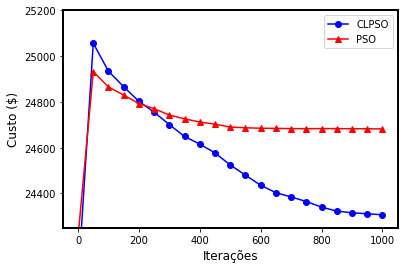
\includegraphics[width=100mm]{images/convergence_13.png}
\fonte{Autor}
\label{conv13}
\end{figure}

Como pode-se notar, nas primeiras iterações, há um aumento do custo nas curvas de convergência. Isso deve-se ao fato de que as soluções iniciais apresentam uma grande penalização, e as partículas tendem a minimizá-la em troca da deterioração do custo de geração. Uma vez que a penalização é reduzida, os custos passam a ter maior importância na função \emph{fitness}. Na média, a partir da iteração de número 100, a função objetivo começa a ser minimizada. A partir da iteração de número 300, pode-se observar a superioridade na capacidade de exploração do algoritmo CLPSO em relação ao PSO, uma vez que o último tende a estagnar precocemente em piores soluções. 

Na Tabela \ref{solucoes13}, podem ser observadas as melhores soluções factíveis obtidas pelos métodos: ED-BFGS, PSO-SQP, CLPSO e CLPSO-SQP. As soluções encontradas pelos métodos ED-BFGS e CLPSO-SQP são muito próximas. Na Tabela \ref{tempo13}, podem ser realizada uma análise comparativa entre os tempos de execução, número de iterações e número de agentes de busca de cada um dos métodos utilizados na análise. Os métodos determinísticos SQP e PDPCBLM tendem a ser mais eficientes no tempo computacional ou no número de iterações, uma vez que utilizam informações provenientes de gradientes, matrizes jacobianas e hessianas que tendem a direcionar o processo de otimização. Os métodos metaheurísticos são mais dispendiosos, pois exigem um maior número de avaliações da função objetivo do problema de otimização. 

Vale ressaltar que a comparação do tempo de execução não é totalmente adequada uma vez que cada autor utilizou diferentes configurações de \emph{hardware}, diferentes \emph{softwares} ou linguagens de programação. Embora o método híbrido tenha apresentado um bom tempo de execução para o caso 1, pode-se observar que a metaheurística PSO obteve um desempenho ainda melhor. Por mais que sejam semelhantes, a estratégia de aprendizagem abrangente do método CLPSO acaba exigindo um maior número de operações no algoritmo, o que justifica o aumento do tempo de execução.



\begin{table}[h!]
\centering
\caption{\label{solucoes13}Melhores soluções obtidas pelos métodos ED-BFGS, PSO-SQP, CLPSO e CLPSO-SQP para o caso 1.}
\begin{tabular}{c c c c c}
	\hline
	\textbf{\makecell{Gerador}} & \textbf{\makecell{ED-BFGS}} &
	\textbf{\makecell{PSO-SQP}} & 
	\textbf{\makecell{CLPSO}} &
	\textbf{\makecell{CLPSO-SQP}} \\
	\hline

	\makecell{$P^G_1$} &  \makecell{628,3185}   & \makecell{628,3205}  & \makecell{628,2551} & \makecell{628,3185}  \\
	
	\makecell{$P^G_2$} &  \makecell{299,1993}   & \makecell{299,0524}  & \makecell{298,9044} & \makecell{299,1993}  \\
	
	\makecel{$P^G_3$} &  \makecell{299,1993}   & \makecell{298,9681}  & \makecell{298,8752} & \makecell{299,1993}  \\
	
    \makecell{$P^G_4$} &  \makecell{159,7331}   & \makecell{159,4680}  & \makecell{159,6652} & \makecell{159,7331} \\

	\makecell{$P^G_5$} &  \makecell{159,7331}   & \makecell{159,1429}  & \makecell{159,7026} & \makecell{159,7331}  \\
	
	\makecell{$P^G_6$} &  \makecell{159,7331}   & \makecell{159,2724}  & \makecell{159,5544} & \makecell{159,7331} \\
	
	\makecell{$P^G_7$} &  \makecell{159,7331}   & \makecell{159,5371}  & \makecell{159,3980} & \makecell{159,7331} \\
	
	\makecell{$P^G_8$} &  \makecell{159,7331}   & \makecell{158,8522}  & \makecell{159,5306} & \makecell{159,7331}  \\
	
	\makecell{$P^G_9$} &  \makecell{159,7331}   & \makecell{159,7845}  & \makecell{159,6242} & \makecell{159,7331}  \\

	\makecell{$P^G_{10}$} &  \makecell{77,39991}   & \makecell{110,9618}  & \makecell{76,7096} & \makecell{77,39991}   \\
	
    \makecell{$P^G_{11}$} &  \makecell{77,39991}   & \makecell{75,0000}  & \makecell{76,2884} & \makecell{77,39991}   \\
    
    \makecell{$P^G_{12}$} &  \makecell{92,39989}   & \makecell{60,0000}  & \makecell{91,6178} & \makecell{92,39991}  \\
    
    \makecell{$P^G_{13}$} &  \makecell{87,68458}   & \makecell{91,6401}  &   \makecell{91,8747} & \makecell{87,68453} \\

    \makecell{$\sum_{i=1}^{n}{P^G_{i}}$} &  \makecell{2520,0000}   & \makecell{2520,0000}  & \makecell{2520,0001} & 2520,0000  \\
    \hline
    
\end{tabular}
\fonte{Autor.}
\end{table}


\begin{table}[h!]
\centering
\caption{\label{tempo13}Dados das performances dos métodos no caso 1.}
\begin{tabular}{c c c c c}
	\hline
	\textbf{\makecell{Método}} & \textbf{\makecell{Tempo \\Médio(s)}} &
	\textbf{\makecell{Desvio \\Padrão(s)}} &
	\textbf{\makecell{Nº de\\ Agentes}} &
	\textbf{\makecell{Nº de \\Iterações}} &
	
	\hline
	
	
	\makecell{EP-SQP\\\tiny{\cite{PSO-SQP}}} &  \makecell{121,93}   & - & 100 & 100 
	\\	
	
	\makecell{PSO-SQP\\\tiny{\cite{PSO-SQP}}} &  \makecell{33,97}   & - & 100 & 100 
	\\	
	
	\makecell{ED-BFGS\\\tiny{\cite{dissertacaojv}}} &  \makecell{22,66}   & - & 100 & 300 
	\\
	
	\makecell{ACO\\\tiny{\cite{POTHIYA2010478}}} &  \makecell{14,35}   & - & - & 100 
	\\
	
	
	\makecell{\textbf{CLPSO-SQP}} &  \makecell{\textbf{13,67}}   & \makecell{\textbf{0,31}} & \textbf{75} & \textbf{1006}
	\\
	\makecell{CLPSO} &  \makecell{13,35}   & \makecell{0,10} & 75 & 1000 
	\\
	\makecell{PSO} &  \makecell{6,47}   & \makecell{0,04} & 75 & 1000 
	\\
	
	\makecell{SQP} &  \makecell{0,31}   & \makecell{0,19} & -& 11\tablefootnote[3]{Número médio de iterações para o método determinístico SQP no caso 1.} 
	\\
	
\makecell{PDPCBLM\\\tiny{\cite{dissertacaodiego}}} &  \makecell{-}   & - & - & 33 
	\\
	
\hline
\end{tabular}
\fonte{Autor.}
\end{table}

\subsection{Caso 2: 19 Unidades Geradoras}

 Para o caso teste com 19 unidades geradoras, foi considerada uma demanda de 2908 MW. Os dados extraídos de \citeonline{balamurugan} dos limites de geração e dos coeficientes da função custo de cada gerador podem ser visualizados na Tabela \ref{19coef}. Além do método híbrido, foram também implementados os métodos PSO, SQP (\emph{solver} APOPT) e CLPSO. Foram realizadas 50 execuções para a coleta de dados, sendo que para o método determinístico SQP foram utilizados 50 pontos iniciais aleatoriamente criados. A formulação matemática e os dados utilizados neste trabalho coincidem com os utilizados nos trabalhos de: \citeonline{dissertacaodiego} (PDPCBLM) e \citeonline{dissertacaojv} (ED e ED-BFGS). 
 
 A Tabela \ref{config19} mostra as configurações de hiperparâmetros utilizados nos métodos PSO e CLPSO. Em ambos os casos foi utilizado um peso de inércia linearmente decrescente. O critério de parada para as metaheurísticas foi de 1000 iterações, com enxames de 100 partículas. Já a Tabela \ref{resultados19} traz os valores obtidos de custo mínimo, custo médio e desvio padrão para cada método utilizado na comparação. 
 
\begin{table}[h!]
\centering
\caption{\label{config19} Hiperparâmetros das metaheurísticas PSO e CLPSO.}

\begin{tabular}{c c c c c c c c c c c }
	\hline
    Método & $c_1$ & $c_2$ & $c$ & $w^{min}$ & $w^{max}$ & $r^{gap}$ & $p_t$ &  \beta & $\Psi$ & $\mu$ \\
    
    PSO & 2 & 2 & - & 0,4 & 0,9 & - & - &  0,1 & 50 & 0,1 \\
    
    CLPSO & - & - & 3 & 0,4  & 0,9 & 3 & 0,4 &  0,1 & 50 & 0,1 \\    
    
    \hline
\end{tabular}
\fonte{Autor.}
\end{table}
 


\begin{table}[h!]
\centering
\caption{\label{resultados19}Valores mínimos, médios e desvios padrão obtidos para a função custo do problema de DE com PCV no caso 2.}

\begin{tabular}{c c c c}
	\hline
	\textbf{\makecell{Método}} & \textbf{\makecell{Custo\\Mínimo (\$)}} &
	\textbf{\makecell{Custo\\Médio (\$)}} & \textbf{\makecell{Desvio\\Padrão (\$)}}\\ 
	\hline

    \makecell{PDPCBLM\\ \tiny\cite{dissertacaodiego}} &  \makecell{17551,0460}   & \makecell{-}  &  -  \\

	\makecell{SQP (APOPT)} &  \makecell{17139,0000}   & \makecell{17847,0000}  &  490,0000  \\
	
    \makecell{ED \\\tiny\cite{dissertacaojv}} &  \makecell{17005,1048}   & \makecell{-}  &  - \\

	\makecell{ED-BFGS \\\tiny\cite{dissertacaojv}} &  \makecell{16982,5601}   & \makecell{-}  &  - \\
	
	\makecell{PSO} &  \makecell{16971,0516}   & \makecell{17070,6077}  &  55,5468  \\
	
	\makecell{CLPSO} &  \makecell{16957,7653}   & \makecell{16979,1733} & 11,8621  \\
	
	\makecell{\textbf{CLPSO-SQP}} &  \makecell{\textbf{16945,6023}}   & \makecell{\textbf{16952,9393}}  &  \textbf{10,9538}
	
}  \\

    \hline
\end{tabular}
\fonte{Autor.}
\end{table}

Novamente, dentre os métodos encontrados na literatura e implementados no trabalho, o algoritmo híbrido desenvolvido foi o que apresentou a melhor solução, ou seja, com os menores custos mínimo, médio e desvio padrão. Os métodos determinísticos PDPCBLM e SQP apresentaram dificuldades em conseguir soluções com baixos valores de custo mínimo. Destaca-se neste caso, que a média do custo obtida pelo método híbrido é melhor do que o custo mínimo obtido por todos os demais métodos do trabalho. A Figura \ref{conv19} ilustra os valores médios da função objetivo da partícula $g^{best}$ em cada uma das iterações das 50 execuções das metaheurísticas CLPSO e PSO.

\begin{figure}[!h]
\centering
\caption{Média das curvas de convergência para as metaheurísticas PSO e CLPSO (caso 2).}
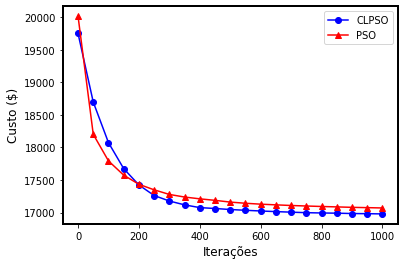
\includegraphics[width=100mm]{images/convergence_19.png}
\fonte{Autor.}
\label{conv19}
\end{figure}

 
\begin{table}[h!]
\centering
\caption{\label{tempo19}Dados das performances dos métodos no caso 2.}
\begin{tabular}{c c c c c}
	\hline
	\textbf{\makecell{Método}} & \textbf{\makecell{Tempo \\Médio(s)}} &
	\textbf{\makecell{Desvio \\Padrão(s)}} &
	\textbf{\makecell{Nº de\\ Agentes}} &
	\textbf{\makecell{Nº de \\Iterações}} &
	
	\hline

	
	\makecell{ED-BFGS\\\tiny{\cite{dissertacaojv}}} &  \makecell{52,30}   & - & 100 & 500 
	\\
	
	\makecell{\textbf{CLPSO-SQP}} &  \textbf{\makecell{13,80}}   & \textbf{\makecell{0,31}} & \textbf{100} & \textbf{1005}
	\\
	\makecell{CLPSO} &  \makecell{13,60}   & \makecell{0,29} & 100 & 1000 
	\\
	

	\makecell{PSO} &  \makecell{8,46}   & \makecell{0,12} & 100 & 1000 
	\\

	\makecell{SQP} &  \makecell{0,21}   & \makecell{0,03} & - & 7\tablefootnote[4]{Número médio de iterações para o método determinístico SQP no caso 2.} 
	\\
	
	\makecell{PDPCBLM\\\tiny{\cite{dissertacaodiego}}} &  \makecell{-}   & - & - & 23 
	\\
\hline
\end{tabular}
\fonte{Autor.}
\end{table}

\begin{table}[h!]
\centering
\caption{\label{solucoes19}Melhores soluções obtidas no caso 2 pelos métodos ED-BFGS, PDPCBLM, CLPSO e CLPSO-SQP.}
\begin{tabular}{c c c c c}
	\hline
	\textbf{\makecell{Gerador}} & \textbf{\makecell{ED-BFGS}} &
	\textbf{\makecell{PDPCBLM}} &
	\textbf{\makecell{CLPSO}} &\textbf{\makecell{CLPSO-SQP}}\\ 
	\hline

	\makecell{$P^G_1$} &  \makecell{104,3720}   & \makecell{200,35634} &  \makecell{100,0250}   &  \makecell{100,0000}  \\
	
	\makecell{$P^G_2$} &  \makecell{371,2835}   & \makecell{308,49096}  & \makecell{371,1949}   &  \makecell{371,3274}  \\
	
	\makecel{$P^G_3$} &  \makecell{249,8589}   & \makecell{226,22324}  &  \makecell{250,0000}   & \makecell{250,0000}  \\
	
    \makecell{$P^G_4$} &  \makecell{24,92514}   & \makecell{25,00000}  & \makecell{25,0000}   &  \makecell{25,0000} \\

	\makecell{$P^G_5$} &  \makecell{63,71548}   & \makecell{63,75000}  &  \makecell{63,4465}   & \makecell{63,7500}  \\
	
	\makecell{$P^G_6$} &  \makecell{269,7616}   & \makecell{186,77848}  & \makecell{270,8865}   &  \makecell{273,3418} \\
	
	\makecell{$P^G_7$} &  \makecell{62,93011}   & \makecell{63,7500}  &  \makecell{63,7500}   & \makecell{63,7500} \\
	
	\makecell{$P^G_8$} &  \makecell{130,1541}   & \makecell{299,37001}  & \makecell{136,1910}   &  \makecell{130,2076}  \\
	
	\makecell{$P^G_9$} &  \makecell{201,1047}   & \makecell{200,0000}  &  \makecell{200,0250}   & \makecell{200,0000}  \\

	\makecell{$P^G_{10}$} &  \makecell{39,59142}   & \makecell{40,0000}  & \makecell{36,8401}   &  \makecell{40,0000}   \\
	
    \makecell{$P^G_{11}$} &  \makecell{149,8667}   & \makecell{150,0000}  & \makecell{150,0000}   &  \makecell{150,0000}   \\
    
    \makecell{$P^G_{12}$} &  \makecell{74,86636}   & \makecell{75,0000}  &  \makecell{75,0000}   & \makecell{75,0000}  \\
    
    \makecell{$P^G_{13}$} &  \makecell{63,7417}   & \makecell{63,7500}  &  \makecell{63,7500}   &   \makecell{63,7500} \\
    
    \makecell{$P^G_{14}$} &  \makecell{94,86275}   & \makecell{95,0000}  &  \makecell{95,0000}   &   \makecell{95,0000} \\
    
    \makecell{$P^G_{15}$} &  \makecell{216,8842}   & \makecell{120,53097}  &  \makecell{216,8654}   &   \makecell{216,8731} \\
    
    \makecell{$P^G_{16}$} &  \makecell{79,6400}   & \makecell{80,0000}  &   \makecell{80,0000}   &  \makecell{80,0000} \\
    
    \makecell{$P^G_{17}$} &  \makecell{79,97481}   & \makecell{80,0000}  &   \makecell{80,0000}   &  \makecell{80,0000} \\
    
    \makecell{$P^G_{18}$} &  \makecell{229,8043}   & \makecell{230,0000}  &  \makecell{230,0000}   &   \makecell{230,0000} \\
    
    \makecell{$P^G_{19}$} &  \makecell{400,3321}   & \makecell{400,0000}  &  \makecell{400,0250}   &   \makecell{400,0000} \\

    \makecell{$\sum_{i=1}^{n}{P^G_{i}}$} &  \makecell{2908,0005}   & \makecell{2908,00009}  & \makecell{2907,9994}   &  2907,9999  \\
    \hline
    
\end{tabular}
\fonte{Autor.}
\end{table}

No caso 2, analisando-se as curvas de convergência, nota-se que ambas as metaheurísticas CLPSO e PSO obtiveram um desempenho parelho, sendo o algoritmo CLPSO o que obteve resultados melhores. Na Tabela \ref{tempo19}, estão detalhados os dados de performance dos métodos desenvolvidos e utilizados na comparação. O método híbrido desenvolvido apresentou tempo de execução aproximadamente 3,8 vezes inferior ao método ED-BFGS. Na Tabela \ref{solucoes19}, podem ser observadas as melhores soluções obtidas pelos métodos: ED-BFGS, PDPCBLM, CLPSO e CLPSO-SQP. 


\subsection{Caso 3: 40 Unidades Geradoras}

 Para o caso teste com 40 unidades geradoras, foi considerada uma demanda de 10500 MW. Os dados extraídos de \citeonline{dados13} dos limites de geração e dos coeficientes da função custo de cada gerador podem ser visualizados na Tabela \ref{40coef}. Além do método híbrido, foram também implementados os métodos PSO, SQP (\emph{solver} APOPT) e CLPSO. Foram realizadas 50 execuções para a coleta de dados, sendo que para o método determinístico SQP foram utilizados 50 pontos iniciais aleatoriamente criados. A formulação matemática e os dados utilizados neste trabalho coincidem com os utilizados nos trabalhos de: \citeonline{PSO-SQP} (PSO-SQP e EP-SQP), \citeonline{pso-gsa} (FPSOGSA), \citeonline{cpso_sqp} (CPSO-SQP), \citeonline{POTHIYA2010478} (ACO) e \citeonline{dissertacaojv} (ED e ED-BFGS). 
 
 A Tabela \ref{config40} mostra as configurações de hiperparâmetros utilizados nos métodos PSO e CLPSO. Em ambos os casos foi utilizado um peso de inércia linearmente decrescente. O critério de parada para as metaheurísticas foi de 1500 iterações, com enxames de 150 partículas. Já a Tabela \ref{resultados40} traz os valores obtidos de custo mínimo, custo médio e desvio padrão para cada método utilizado na comparação. 
 

\begin{table}[h!]
\centering
\caption{\label{config40} Hiperparâmetros das metaheurísticas PSO e CLPSO.}

\begin{tabular}{c c c c c c c c c c c }
	\hline
    Método & $c_1$ & $c_2$ & $c$ & $w^{min}$ & $w^{max}$ & $r^{gap}$ & $p_t$ &  \beta & $\Psi$ & $\mu$ \\
    
    PSO & 2 & 2 & - & 0,4 & 0,9 & - & - &  0,1 & 50 & 0,25 \\
    
    CLPSO & - & - & 1 & 0,4  & 0,9 & 0 & 0,4 &  0,1 & 50 & 0,25 \\    
    
    \hline
\end{tabular}
\fonte{Autor.}
\end{table}

\begin{table}[h!]
\centering
\caption{\label{resultados40}Valores mínimos, médios e desvios-padrão obtidos para a função custo do problema de DE com PCV no caso 3.}

\begin{tabular}{c c c c}
	\hline
	\textbf{\makecell{Método}} & \textbf{\makecell{Custo\\Mínimo (\$)}} &
	\textbf{\makecell{Custo\\Médio (\$)}} & \textbf{\makecell{Desvio\\Padrão (\$)}}\\ 
	\hline


    \makecell{PSO} &  \makecell{123625,7589}   & \makecell{126154,6419}  &  1282,5075  \\
    

	\makecell{SQP (APOPT)} &  \makecell{123138,3542}   & \makecell{125390,2253}  &  1035,9314  \\
	
    \makecell{EP-SQP\\\tiny{\cite{PSO-SQP}}} &  \makecel{122323,9700}   & \makecell{122379,6300}  &  -  \\
    
	\makecell{PSO-SQP\\\tiny{\cite{PSO-SQP}}} &  \makecell{122094,6700}   & \makecell{122245,2500}  &  -  \\
	
	\makecell{{ACO}\\\tiny{\cite{POTHIYA2010478}}} &  \makecell{{121532,6736}}   & \makecell{{121606,4500}}  &  {7,86}\\
	
    \makecell{ED \\\tiny{\cite{dissertacaojv}}} &  \makecell{121508,0200}   & \makecell{-}  &  - \\

	\makecell{ED-BFGS \\\tiny{\cite{dissertacaojv}}} &  \makecell{121490,9216}   & \makecell{-}  &  - \\
	
	\makecell{CLPSO} &  \makecell{121485,1093}   & \makecell{121537,8301} & 75,5028  \\
	
	\makecell{CPSO\\\tiny\cite{cpso_sqp}} &  \makecell{121481,6201}   & \makecell{121865,2300} & 114,6500  \\
	

	\makecell{\textbf{CLPSO-SQP}} &  \makecell{\textbf{121476,6736}}   & \makecell{\textbf{121496,0788}}  &  \textbf{35,3006}\\

	
		\makecell{CPSO-SQP\\\tiny\cite{cpso_sqp}} &  \makecell{121458,5400}   & \makecell{122028,1600} & -  \\
	
	\makecell{FPSOGSA\\\tiny{\cite{pso-gsa}}}} &  \makecell{121412,5421}   & \makecell{121413,561938}  &  -
	
}  \\

    \hline
\end{tabular}
\fonte{Autor.}
\end{table}

Neste caso de teste, o método híbrido desenvolvido apresentou a segunda melhor performance dentre os métodos utilizados na comparação. Embora tenha obtido um valor de custo mínimo pior que o do método CPSO-SQP, pode-se notar que o algoritmo CLPSO-SQP obteve um menor valor de custo médio, o que indica uma melhor performance. Ainda, analisando-se a Tabela \ref{solucoes40} com as quatro melhores soluções reportadas pelos autores dos métodos, observa-se que a solução encontrada por \citeonline{pso-gsa} (FPSO-GSA) está muito próxima à solução obtida pelo método híbrido implementado. 


\begin{table}[h!]
\centering
\caption{\label{solucoes40}Melhores soluções obtidas no caso 3 pelos métodos ED-BFGS, FPSOGSA, CLPSO e CLPSO-SQP.}
\begin{tabular}{c c c c c}
	\hline
	\textbf{\makecell{Gerador}} & \textbf{\makecell{ED-BFGS}} &
	\textbf{\makecell{FPSOGSA}} &
	\textbf{\makecell{CLPSO}} &\textbf{\makecell{CLPSO-SQP}}\\ 
	\hline

	\makecell{$P^G_1$} &  \makecell{110,7998}   & \makecell{110,7998} &  \makecell{111,3741} &  \makecell{110,7998}  \\
	
	\makecell{$P^G_2$} &  \makecell{110,7998}   & \makecell{110,7998}  &  \makecell{111,6252} &  \makecell{110,7998}  \\
	
	\makecel{$P^G_3$} &  \makecell{97,39975}   & \makecell{97,3999}  &  \makecell{97,5025} &  \makecell{97,3999}  \\
	
    \makecell{$P^G_4$} &  \makecell{179,7236}   & \makecell{179,7331 } &  \makecell{179,7622} &  \makecell{179,7331} \\

	\makecell{$P^G_5$} &  \makecell{87,79993}   & \makecell{87,7999} &  \makecell{92,1330} &  \makecell{87,7999}  \\
	
	\makecell{$P^G_6$} &  \makecell{140,0000}   & \makecell{140,0000} &  \makecell{139,9986} &  \makecell{140,0000} \\
	
	\makecell{$P^G_7$} &  \makecell{259,6003}   & \makecell{259,5997}  &  \makecell{299,9846}&  \makecell{300,0000} \\
	
	\makecell{$P^G_8$} &  \makecell{280,5996}   & \makecell{284,5997} &  \makecell{284,7213} &  \makecell{284,5997}  \\
	
	\makecell{$P^G_9$} &  \makecell{284,5996}   & \makecell{284,5997} &  \makecell{284,7357} &  \makecell{284,5997}  \\

	\makecell{$P^G_{10}$} &  \makecell{130,0002}   & \makecell{130,0000} &  \makecell{130,0140} &  \makecell{130,0000}   \\
	
    \makecell{$P^G_{11}$} &  \makecell{168,7977}   & \makecell{94,0000} &  \makecell{94,0375} &  \makecell{94,0000}   \\
    
    \makecell{$P^G_{12}$} &  \makecell{168,7977}   & \makecell{94,0000} &  \makecell{94,0156} &  \makecell{94,0000}  \\
    
    \makecell{$P^G_{13}$} &  \makecell{304,5196}   & \makecell{214,7598} &  \makecell{125,0149} &    \makecell{125,0000} \\
    
    \makecell{$P^G_{14}$} &  \makecell{304,5196}   & \makecell{394,2794} &  \makecell{394,2829} &    \makecell{394,2794} \\
    
    \makecell{$P^G_{15}$} &  \makecell{304,5196}   & \makecell{394,2794} &  \makecell{394,2822} &    \makecell{394,2794} \\
    
    \makecell{$P^G_{16}$} &  \makecell{304,5196}   & \makecell{394,2794} &  \makecell{394,2815} &    \makecell{394,2794} \\
    
    \makecell{$P^G_{17}$} &  \makecell{489,2163}   & \makecell{489,2794 } &  \makecell{489,2882} &    \makecell{489,2794} \\
    
    \makecell{$P^G_{18}$} &  \makecell{489,2163}   & \makecell{489,2794 } &  \makecell{489,2913} &    \makecell{489,2794} \\
    
    \makecell{$P^G_{19}$} &  \makecell{511,2794}   & \makecell{511,2794} &  \makecell{511,3160} &    \makecell{511,2794} \\

    \makecell{$P^G_{20}$} &  \makecell{511,2794}   & \makecell{511,2794} &  \makecell{511,3172} &    \makecell{511,2794} \\


    \makecell{$P^G_{21}$} &  \makecell{523,2822}   & \makecell{523,2794} &  \makecell{523,3187} &    \makecell{523,2794} \\
    

    \makecell{$P^G_{22}$} &  \makecell{523,2822}   & \makecell{523,2794} &  \makecell{523,3035} &    \makecell{523,2794} \\
    

    \makecell{$P^G_{23}$} &  \makecell{523,2822}   & \makecell{523,2794} &  \makecell{523,3692} &    \makecell{523,2794} \\
    

    \makecell{$P^G_{24}$} &  \makecell{523,2822}   & \makecell{523,2794} &  \makecell{523,4028} &    \makecell{523,2794} \\
    

    \makecell{$P^G_{25}$} &  \makecell{523,2822}   & \makecell{523,2794} &  \makecell{523,3203} &    \makecell{523,2794} \\
    

    \makecell{$P^G_{26}$} &  \makecell{523,2822}   & \makecell{523,2794} &  \makecell{523,3133} &    \makecell{523,2794} \\
    

    \makecell{$P^G_{27}$} &  \makecell{10,00004}   & \makecell{10,0000} &  \makecell{10,0083} &    \makecell{10,0000} \\
    

    \makecell{$P^G_{28}$} &  \makecell{10,00004}   & \makecell{10,0000} &  \makecell{10,0093} &    \makecell{10,0000} \\
    

    \makecell{$P^G_{29}$} &  \makecell{10,00004}   & \makecell{10,0000} &  \makecell{10,0178} &    \makecell{10,0000} \\
    

    \makecell{$P^G_{30}$} &  \makecell{87,79993}   & \makecell{87,7999}  &  \makecell{89,7244}&    \makecell{96,3569} \\
    

    \makecell{$P^G_{31}$} &  \makecell{189,9999}   & \makecell{190,0000} &  \makecell{189,9987} &    \makecell{190,0000} \\
    

    \makecell{$P^G_{32}$} &  \makecell{189,9999}   & \makecell{190,0000} &  \makecell{189,9957} &    \makecell{190,0000} \\
    

    \makecell{$P^G_{33}$} &  \makecell{189,9999}   & \makecell{190,0000} &  \makecell{189,9887} &    \makecell{190,0000} \\
    

    \makecell{$P^G_{34}$} &  \makecell{196,4129}   & \makecell{164,7998} &  \makecell{199,9976} &    \makecell{200,0000} \\
    

    \makecell{$P^G_{35}$} &  \makecell{196,4129}   & \makecell{200,0000} &  \makecell{199,9927} &    \makecell{200,0000} \\
    

    \makecell{$P^G_{36}$} &  \makecell{196,4129}   & \makecell{194,3973} &  \makecell{199,9934} &    \makecell{200,0000} \\
    

    \makecell{$P^G_{37}$} &  \makecell{109,9999}   & \makecell{110,0000} &  \makecell{109,992} &    \makecell{110,0000} \\
    

    \makecell{$P^G_{38}$} &  \makecell{109,9999}   & \makecell{110,0000} &  \makecell{109,9993} &    \makecell{110,0000} \\
    

    \makecell{$P^G_{39}$} &  \makecell{109,9999}   & \makecell{110,0000} &  \makecell{109,9876} &    \makecell{110,0000} \\
    

    \makecell{$P^G_{40}$} &  \makecell{511,2794}   & \makecell{511,2794} &  \makecell{511,2876} &    \makecell{511,2794} \\
    

    \makecell{$\sum_{i=1}^{n}{P^G_{i}}$} &  \makecell{10499,9991}   & \makecell{10500,0000} &  \makecell{10499,9994}  &  10500,0004  \\
    \hline
    
\end{tabular}
\fonte{Autor.}
\end{table}


\begin{table}[h!]
\centering
\caption{\label{tempos40}Dados das performances dos métodos no caso 3.}
\begin{tabular}{c c c c c}
	\hline
	\textbf{\makecell{Método}} & \textbf{\makecell{Tempo \\Médio(s)}} &
	\textbf{\makecell{Desvio \\Padrão(s)}} &
	\textbf{\makecell{Nº de\\ Agentes}} &
	\textbf{\makecell{Nº de \\Iterações}} &
	
	\hline


    \makecell{EP-SQP\\\tiny{\cite{PSO-SQP}}} &  \makecell{997,73}   & \makecell{-} & 100 & 100
	\\
	
  \makecell{PSO-SQP\\\tiny{\cite{PSO-SQP}}} &  \makecell{733,97}   & \makecell{-} & 100 & 100 
	\\

	
	\makecell{ACO\\\tiny{\cite{POTHIYA2010478}}} &  \makecell{52,45}   & \makecell{-} & - & 500 
	\\	
	\makecell{CPSO-SQP\\\tiny{\cite{cpso_sqp}}} &  \makecell{98,49}   & \makecell{-} & 100 & 200 
	\\
	
\makecell{FPSOGSA\\\tiny{\cite{pso-gsa}}} &  \makecell{-}   &  \makecell{-} & 300 & 1000 
\\

	\makecell{ED-BFGS\\\tiny{\cite{dissertacaojv}}} &  \makecell{90,32}   & - & 200 & 6000 
	\\
	
	\makecell{PSO} &  \makecell{62,29}   & \makecell{0,33} & 150 & 1500 
	\\

	\makecell{CLPSO} &  \makecell{90,77}   & \makecell{0,72} & 150 & 1500 
	\\
	\makecell{SQP} &  \makecell{0,37}   & \makecell{0,05} & - & 15\tablefootnote[5]{Número médio de iterações para o método determinístico no caso 3.} 
	\\
	
	\makecell{CLPSO-SQP} &  \makecell{91,20}   & \makecell{0,78} & 150 & 1513 
	\\

\hline
\end{tabular}
\fonte{Autor.}
\end{table}


A Figura \ref{conv40} ilustra os valores médios da função objetivo da partícula $g^{best}$ em cada uma das iterações das 50 execuções das metaheurísticas CLPSO e PSO. Assim como no caso 1, pode-se observar a superioridade de exploração global da metaheurística CLPSO que, na média, obteve custos de geração muito inferiores. 


\begin{figure}[!h]
\centering
\caption{Média das curvas de convergência para as metaheurísticas PSO e CLPSO (caso 3).}
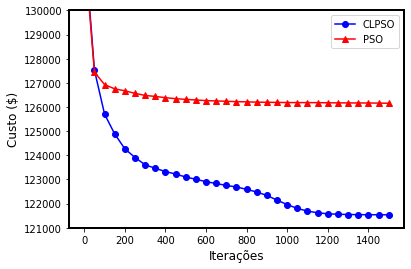
\includegraphics[width=100mm]{images/convergence_40.png}
\fonte{Autor.}
\label{conv40}
\end{figure}


Conforme pode-se observar na Tabela \ref{tempos40}, o tempo de execução obtido pelo algoritmo é semelhante ao dos métodos CPSO-SQP e ED-BFGS. Considerando os testes e comparações realizadas com o algoritmo híbrido CLPSO-SQP nesta seção, conclui-se que o método proposto mostrou-se competitivo obtendo resultados satisfatórios quando comparados a outros métodos determinísticos, metaheurísticos ou híbridos da literatura. Como observado, a metaheurística CLPSO realiza uma busca global no hiperespaço de soluções do problema e, em seguida, o método determinístico SQP aprimora localmente a solução. Quando comparadas as soluções obtidas pelo método híbrido com as dos métodos SQP e CLPSO separados, fica evidente que ambos se beneficiam da hibridização proposta.

Quando analisada a arquitetura híbrida que utiliza recorrentemente o método determinístico para aprimorar soluções durante a execução da metaheurística, conforme proposto por \citeonline{dissertacaojv} (ED-BFGS), \citeonline{cpso_sqp} (CPSO-SQP) e \citeonline{PSO-SQP} (PSO-SQP e EP-SQP), pode-se observar uma elevação do tempo de execução requerido e uma performance média na otimização do custo que é inferior à da arquitetura proposta neste trabalho. Isso deve-se ao fato de que algumas metaheurísticas são mais propensas a direcionar o processo de busca para a posição do agente melhor avaliado do grupo, que tende a ser a solução aperfeiçoada pelo método determinístico. No entanto, em um problema não convexo e multimodal, esta solução pode estar em uma região distante da solução ótima, o que acaba interferindo no processo de busca dos agentes direcionando-os a uma região não promissora do hiperespaço de soluções.

Na próxima seção, serão apresentados os resultados dos testes numéricos utilizando o método hibrido para o problema de DE com PCV, ZOP e RT nos sistemas IEEE de 14 e 30 barras.


\section{Despacho Econômico com Ponto de Carregamento de Válvula, Zonas de Operação Proibidas e Representação da Transmissão}

No Apêndice B, são apresentados os dados dos sistemas IEEE de 14 e 30 barras. Para os casos testes do problema DE com PCV, ZOP e RT, foram utilizadas as tolerâncias $\tau_p = 10^{-7}$ com $\tau_q = 10^{-7}$ para o método FD e $\tau_{opt} = 10^{-7}$ com $\tau_{fact} = 10^{-7}$ para o método SQP. Para execução do método BB, foi definida uma tolerância $\tau_{int} = 10^{-5}$ de desvio para as variáveis discretas para uma solução ser considerada factível e foi utilizada a estratégia de busca adaptativa na exploração dos nós. Nas metaheurísticas, foram consideradas infactíveis soluções com ultrapassagens superiores a $10^{-7}$ dos limites das variáveis dependentes dos sistemas.

\subsection{Caso 1: Sistema Elétrico IEEE de 14 Barras}

O sistema IEEE de 14 barras tem os seguintes elementos:

\begin{itemize}
    \item 1 barra de geração \emph{slack};
    \item 4 barras de geração com controle de reativos;
    \item 9 barras de carga;
    \item 20 linhas de transmissão;
    \item 3 transformadores com \emph{tap} variável;
    \item 1 banco de capacitores \emph{shunt} variável.
\end{itemize}

Os coeficientes $a_k$, $b_k$ e $c_k$ da porção quadrática da função custo de geração foram retirados do banco de dados do pacote \emph{pandapower}. Já os coeficientes $e_k$ e $f_k$ da porção referente aos efeitos de PCV foram estimados conforme proposto no trabalho de \citeonline{pinheiro}. Cada gerador do sistema possui três ZOP, também definidas conforme equação proposta no trabalho de \citeonline{pinheiro}. As ZOP utilizadas podem ser visualizadas na Tabela \ref{ZOPieee14}:


\begin{table}[h]
\caption{\label{ZOPieee14}ZOP dos geradores do sistema elétrico IEEE de 14 barras.}
\center
\begin{tabular}{c c c c}
\hline
 \rule{0mm}{3ex} Barra  & $(\underline{P^G_{k,1}}, \overline{P^G_{k,1}})$ (MW) & $(\underline{P^G_{k,2}}, \overline{P^G_{k,2}})$ (MW)& $(\underline{P^G_{k,3}}, \overline{P^G_{k,3}})$ (MW)
 \\[2mm]
 \hline
 
1& (47,4857; 94,9714) & (142,4571; 189,9429) & (237,4286; 284,9143) \\
2& (20; 40) & (60; 80)& (100; 120) \\
3& (14,2857; 28,5714) & (42,8571; 57,1429)& (71,4286; 85,7143) \\
6& (14,2857; 28,5714) & (42,8571; 57,1429)& (71,4286; 85,7143) \\
8& (14,2857; 28,5714) & (42,8571; 57,1429)& (71,4286; 85,7143) \\
\hline
\end{tabular}
\fonte{Autor.}
\end{table}

Na modelagem, considerou-se que a magnitude de tensão nas barras tem como
limites mínimos e máximos 0,95 e 1,05 \emph{pu}, respectivamente. Além disso, os \emph{taps} dos transformadores ($t_{4,7}$, $t_{4,9}$ e $t_{5,6}$) devem pertencer ao conjunto discreto \{0,90; 0,91; 0,92; 0,93; 0,94; 0,95; 0,96; 0,97; 0,98; 0,99; 1,0; 1,01; 1,02; 1,03; 1,04; 1,05; 1,06; 1,07; 1,08; 1,09; 1,1\} \emph{pu}. Já a susceptância \emph{shunt} ($b^{sh}_9$) do banco de capacitores deve pertencer ao conjunto discreto \{0; 0,01; 0,02; 0,03; 0,04; 0,05\} \emph{pu} \cite{antlion}.

Além do método híbrido, foram também implementados os métodos PSO, SQP-BB
(\emph{solver} APOPT) e CLPSO. Foram realizadas 50 execuções para a coleta de dados, sendo que para o método determinístico SQP-BB foram utilizados 50 pontos iniciais aleatoriamente criados. Na formulação matemática do problema, para o método SQP-BB, foram utilizadas variáveis binárias artificiais para tratar as restrições de ZOP, assim como a estratégia estabelecida por \citeonline{pan2018hybrid} para tratar a não diferenciabilidade da função objetivo. Os parâmetros utilizados pelas metaheurísticas PSO e CLPSO encontram-se na Tabela \ref{configieee14}. Foram utilizados enxames com 15 partículas e 120 iterações, com pesos de inércia linearmente decrescentes. No método híbrido, após encontrar as soluções pelo método CLPSO, os conjuntos de variáveis discretas foram reduzidos aos 4 vizinhos imediatamente inferiores e superiores possíveis para os \emph{taps} e \emph{shunts} de $g^{best}$, a fim de executar o método SQP-BB.


\begin{table}[h!]
\centering
\caption{\label{configieee14} Hiperparâmetros das metaheurísticas PSO e CLPSO.}

\begin{tabular}{c c c c c c c c c c c c c}
	\hline
    Método & $c_1$ & $c_2$ & $c$ & $w^{min}$ & $w^{max}$ & $r^{gap}$ & $p_t$ & \mu& \beta & $\zeta$ & $\omega$ & $\chi$ \\
    
    PSO & 2 & 2 & - & 0,4 & 0,9 & - & - & 0,25& 0,1 & $10^6$ & $10^2$ & $10^6$ \\
    
    CLPSO & - & - & 2 & 0,4  & 0,9 & 0 & 0,9 &  0,25 & 0,1  & $10^6$ & $10^2$ & $10^6$ \\    
    
    \hline
\end{tabular}
\fonte{Autor.}
\end{table}
A Tabela \ref{results_ieee14} mostra as estatísticas de desempenho na otimização do custo para todos os métodos testados no sistema IEEE de 14 barras, considerando apenas soluções factíveis. Já a Tabela \ref{temposieee14}, mostra as médias e desvios padrão de tempo de execução, número de agentes de busca e iterações de cada método.

\begin{table}[h!]
\centering
\caption{\label{results_ieee14}Valores mínimos, médios e desvios padrão obtidos para a função custo do problema de DE com PCV, ZOP e RT no sistema IEEE de 14 barras.}

\begin{tabular}{c c c c c}
	\hline
	\textbf{\makecell{Método}} & \textbf{\makecell{Custo\\Mínimo (\$)}} &
	\textbf{\makecell{Custo\\Médio (\$)}} & \textbf{\makecell{Desvio\\Padrão (\$)}} & \textbf{\makecell{Taxa de\\ Sucesso (\%)}}\\ 
	\hline

	\makecell{PSO} &  \makecell{8437,9364}   & \makecell{8693,7874}  & \makecell{261,9726} & 66 \\

	\makecell{CLPSO} &  \makecell{8437,1786}   & \makecell{8483,0977}  & \makecell{91,6669}& 64 \\
	
	\makecell{SQP-BB (APOPT)} &  \makecell{8436,9120}   & \makecell{8589,7214}  & 142,0256  & 98 \\
	
	\makecell{\textbf{CLPSO-SQP-BB}} &  \makecell{\textbf{8436,9120}}   & \makecell{\textbf{8506,6708}}  &  \textbf{116,9647} & \textbf{100} \\
	\hline
\end{tabular}
\fonte{Autor.}
\end{table}


\begin{table}[h!]
\centering
\caption{\label{temposieee14}Dados das performances dos métodos no sistema IEEE de 14 barras.}
\begin{tabular}{c c c c c}
	\hline
	\textbf{\makecell{Método}} & \textbf{\makecell{Tempo \\Médio(s)}} &
	\textbf{\makecell{Desvio \\Padrão(s)}} &
	\textbf{\makecell{Nº de\\ Agentes}} &
	\textbf{\makecell{Nº de \\Iterações}} &
	
	\hline

	\makecell{PSO} &  \makecell{29,14}   & \makecell{4,72} & 15 & 120 
	\\

	\makecell{CLPSO} &  \makecell{29,36}   & \makecell{1,91} & 15 & 120 
	\\
	\makecell{SQP-BB (APOPT)} &  \makecell{55,18}   & \makecell{35,92} & - & 6\tablefootnote[6]{Número médio de iterações para o método determinístico no sistema IEEE de 14 barras.} 
	\\
	
	\makecell{CLPSO-SQP-BB} &  \makecell{36,67}   & \makecell{2,12} & 15 & 126\tablefootnote[7]{Número médio de iterações para o método híbrido no sistema IEEE de 14 barras.}
	\\

\hline
\end{tabular}
\fonte{Autor.}
\end{table}

Analisando-se as Tabelas \ref{results_ieee14} e \ref{temposieee14}, pode-se observar que o método híbrido juntamente com o método determinístico encontraram as melhores soluções para o problema em questão. O método híbrido desenvolvido, em relação ao método determinístico, obteve uma menor média e desvio padrão do custo total de geração, além de uma maior taxa de sucesso na obtenção de soluções factíveis e um menor tempo médio de execução. Em relação as metaheurísticas, o método híbrido obteve uma maior média de custos quando comparado ao método CLPSO, no entanto, a taxa de obtenção de soluções factíveis foi consideravelmente maior. Para aprimorar a taxa de sucesso das metaheurísticas é necessário aumentar os parâmetros de penalização da função \emph{fitness} do algoritmo, o que acarreta na obtenção de soluções factíveis mas com degeneração dos valores médios da função objetivo.

A Figura \ref{ieee_14_curves} ilustra os valores médios da função objetivo da partícula $g^{best}$ em cada
uma das iterações das execuções das metaheurísticas PSO e CLPSO que obtiveram soluções factíveis. Pode-se observar que a partir da iteração de número 20, o método CLPSO tende a continuar melhorando a função objetivo do problema de forma mais acentuada que o algoritmo PSO.

\begin{figure}[h!]
    \caption{\label{ieee_14_curves}Média das curvas de convergência para as metaheurísticas PSO e CLPSO no sistema IEEE de 14 barras.}
    \centering
    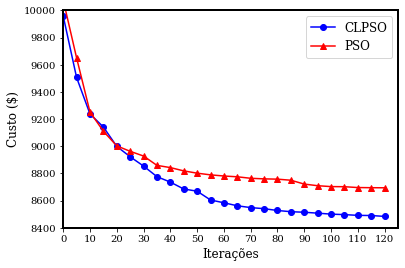
\includegraphics[width=100mm]{images/custo_medio_ieee14.png}
   
\fonte{Autor.}
\end{figure}

Nas Tabelas \ref{Pieee14} e \ref{Qieee14} estão os dados de potência ativa e reativa das melhores soluções factíveis de todos os métodos desenvolvidos no trabalho. Pode-se visualizar na Tabela \ref{Pieee14} que os melhores valores de potência ativa obtidos por cada método são semelhantes, sendo a geração da barra \emph{slack} a única a apresentar diferenças. Tais diferenças são resultantes das perdas de potência ativa nas linhas de transmissão, que acabam sendo supridas pelo gerador de tal barra. Os métodos determinístico e híbrido foram os que melhor conseguiram minimizar tal critério de forma indireta, uma vez que a função objetivo do problema é o custo total de geração e a geração é dependente das perdas do sistema. Neste sentido, vale ressaltar a vantagem da hibridização proposta, uma vez que a metaheurística encontra uma solução de boa qualidade e o método determinístico a aprimora localmente, realizando um ajuste preciso das variáveis do problema. Além disso, todas as potências encontradas estão fora das ZOP estabelecidas na Tabela \ref{ZOPieee14}. Pode-se observar também, através da Tabela \ref{Qieee14}, que as potências reativas encontradas por cada método encontram-se dentro dos limites estabelecidos pelos dados do sistema elétrico no Apêndice B.


\begin{table}[h!]
\centering
\caption{\label{Pieee14}Soluções de potência ativa obtidas pelos métodos PSO, SQP-BB, CLPSO e CLPSO-SQP-BB no sistema IEEE de 14 barras.}
\begin{tabular}{c c c c c}
	\hline
	\textbf{\makecell{Variável (MW)}} & \textbf{\makecell{PSO}} &
	\textbf{\makecell{SQP-BB}} &
	\textbf{\makecell{CLPSO}} &\textbf{\makecell{CLPSO-SQP-BB}}\\ 
	\hline

 \rule{0mm}{3ex} $P^G_1$& 232,7968 & 232,7641& 232,7726 & 232,7641\\[2mm]
$P^G_2$ & 40,0000 & 40,0000 & 40,0000& 40,0000 \\[2mm]
$P^G_3$ & 0,0000 &0,0000 & 0,0000 & 0,0000 \\[2mm]
$P^G_6$  & 0,0000 &0,0000 & 0,0000& 0,0000 \\[2mm]
$P^G_8$  & 0,0000 &0,0000 & 0,0000& 0,0000 \\[2mm]
Total  & 272,7968 & 272,7641& 272,7726& 272,7641 \\ [2mm]
Demanda & 259,0000 &259,0000 & 259,0000& 259,0000\\[2mm]
Perdas & 13,7968 & 13,7641 & 13,7726& 13,7641 \\[2mm]
\hline
\end{tabular}
\fonte{Autor.}
\end{table}


\begin{table}[h!]
\centering
\caption{\label{Qieee14}Soluções de potência reativa obtidas pelos métodos PSO, SQP-BB, CLPSO e CLPSO-SQP-BB no sistema IEEE de 14 barras.}
\begin{tabular}{c c c c c}
	\hline
	\textbf{\makecell{Variável (MVAr)}} & \textbf{\makecell{PSO}} &
	\textbf{\makecell{SQP-BB}} &
	\textbf{\makecell{CLPSO}} &\textbf{\makecell{CLPSO-SQP-BB}}\\ 
	\hline

 \rule{0mm}{3ex}
$Q^G_1 $ & 0,0311& 0,0000 &0,8310 & 0,0000 \\[2mm]
$Q^G_2$ &26,3280& 24,8852& 26,3365& 24,8852\\[2mm]
$Q^G_3$ &30,0802 & 31,1040& 29,2567	& 31,1040 \\[2mm]
$Q^G_6 $ & 23,3803& 24,0000& 23,8471& 24,0000 \\[2mm]
$Q^G_8$ &22,0175& 24,0000& 23,0763& 24,0000\\[2mm]
\hline
\end{tabular}
\fonte{Autor.}
\end{table}


Na Tabela \ref{tebshieee14} estão os dados das variáveis discretas das melhores soluções de cada método. Novamente, pode-se observar que os valores estão muito próximos, uma vez que as melhores soluções de todos os métodos obtiveram custos semelhantes. 

\begin{table}[h!]
\centering
\caption{\label{tebshieee14}Soluções de \emph{tap} e susceptância \emph{shunt}  obtidas pelos métodos PSO, SQP-BB, CLPSO e CLPSO-SQP-BB no sistema IEEE de 14 barras.}
\begin{tabular}{c c c c c}
	\hline
	\textbf{\makecell{Variável (\emph{pu})}} & \textbf{\makecell{PSO}} &
	\textbf{\makecell{SQP-BB}} &
	\textbf{\makecell{CLPSO}} &\textbf{\makecell{CLPSO-SQP-BB}}\\ 
	\hline

$t_{4,7}$ &1,00&1,03 &1,02& 1,03\\
$t_{4,9}$ &0,97&0,90 &0,91& 0,90\\
$t_{5,6}$ &0,98&0,99 &0,99& 0,99\\
$b^{sh}_9$ &0,05&0,05&0,05& 0,05\\
\hline
\end{tabular}
\fonte{Autor.}
\end{table}

Nas Figuras \ref{ieee_14_volt} e \ref{ieee_14_ang} estão, respectivamente, os dados de manitude e ângulo de tensão das melhores soluções obtidas pelos métodos CLPSO e CLPSO-SQP-BB. Assim como as demais variáveis, pode-se observar uma grande semelhança entre os valores obtidos.

\begin{figure}[h]
    \caption{\label{ieee_14_volt}Magnitudes de tensão obtidas pelos métodos CLPSO e CLPSO-SQP-BB no sistema IEEE de 14 barras.}
    \centering
    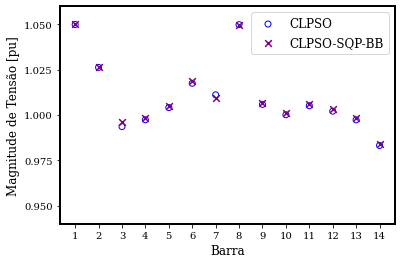
\includegraphics[width=100mm]{images/tensoes_ieee14.png}
   
\fonte{Autor.}
\end{figure}

\begin{figure}[h]
    \caption{\label{ieee_14_ang}Ângulos de tensão obtidos pelos métodos CLPSO e CLPSO-SQP-BB no sistema IEEE de 14 barras}
    \centering
    \includegraphics[width=100mm]{images/ângulos_ieee14.png}
   
\fonte{Autor.}
\end{figure}


De forma geral, para o sistema IEEE de 14 barras, o método híbrido proposto obteve resultados que justificam sua superioridade em relação aos demais métodos. Obteve médias menores que as dos métodos PSO e SQP-BB e custos mínimos inferiores aos métodos PSO e CLPSO. Além disso, foi o algoritmo que apresentou maior taxa de sucesso na obtenção de soluções factíveis.  O tempo de execução do método híbrido foi inferior ao do método determinístico, o que mostra que a estratégia de \emph{warm-start} acarreta em um menor número de iterações para o método SQP-BB. A metaheurística CLPSO se complementa com o método SQP-BB, uma vez que o método determinístico é ineficiente em explorar globalmente o espaço de soluções do problema e a metaheurística não é eficiente na exploração local. 


\subsection{Caso 2: Sistema Elétrico IEEE de 30 Barras}


O sistema IEEE de 30 barras tem os seguintes elementos:

\begin{itemize}
    \item 1 barra de geração \emph{slack};
    \item 5 barras de geração com controle de reativos;
    \item 24 barras de carga;
    \item 37 linhas de transmissão;
    \item 4 transformadores com \emph{tap} variável;
    \item 2 banco de capacitores \emph{shunt} variável.
\end{itemize}

Os coeficientes $a_k$, $b_k$ e $c_k$ da porção quadrática da função custo de geração foram retirados do banco de dados do pacote \emph{pandapower}. Já os coeficientes $e_k$ e $f_k$ da porção referente aos efeitos de PCV foram estimados conforme técnica proposta no trabalho de \citeonline{pinheiro}. As ZOP utilizadas podem ser visualizadas na Tabela \ref{ZOPieee30}:


\begin{table}[h]
\caption{\label{ZOPieee30}ZOP dos geradores do sistema elétrico IEEE de 30 barras.}
\center
\begin{tabular}{c c c}
\hline
 \rule{0mm}{3ex} Barra  & $(\underline{P^G_{k,1}}, \overline{P^G_{k,1}})$ (MW) & $(\underline{P^G_{k,2}}, \overline{P^G_{k,2}})$ (MW)
 \\[2mm]
 \hline
 
1& (55; 66) & (80; 120)  \\
2& (21; 24) & (45; 55)  \\
5& (30; 36) & -  \\
8& (25; 30) & -  \\
11& (25; 28) & -  \\
13& (24; 30) & -\\
\hline
\end{tabular}
\fonte{\citeonline{kasma}}
\end{table}

Na modelagem, considerou-se que a magnitude de tensão nas barras tem como
limites mínimos e máximos 0,95 e 1,05 \emph{pu}, respectivamente. Além disso, os \emph{taps} dos transformadores ($t_{6,9}$, $t_{6,10}$, $t_{4,12}$ e $t_{28,27}$) devem pertencer ao conjunto discreto \{0,90; 0,91; 0,92; 0,93; 0,94; 0,95; 0,96; 0,97; 0,98; 0,99; 1,0; 1,01; 1,02; 1,03; 1,04; 1,05; 1,06; 1,07; 1,08; 1,09; 1,1\} \emph{pu}. Já as susceptâncias \emph{shunt} ($b^{sh}_{10}$ e $b^{sh}_{24}$) dos bancos de capacitores devem pertencer ao conjunto discreto \{0; 0,01; 0,02; 0,03; 0,04; 0,05\} \emph{pu} \cite{antlion}.

Além do método híbrido, foram também implementados os métodos PSO, SQP-BB
(\emph{solver} APOPT) e CLPSO. Foram realizadas 50 execuções para a coleta de dados, sendo que para o método determinístico SQP-BB foram utilizados 50 pontos iniciais aleatoriamente criados. Na formulação matemática do problema, para o método SQP-BB, foram utilizadas variáveis binárias artificiais para tratar as restrições de ZOP, assim como a estratégia estabelecida por \citeonline{pan2018hybrid} para tratar a não diferenciabilidade da função objetivo. Os parâmetros utilizados pelas metaheurísticas PSO e CLPSO encontram-se na Tabela \ref{configieee30}. Foram utilizados enxames com 20 partículas e 150 iterações, com pesos de inércia linearmente decrescentes. No método híbrido, após encontrar as soluções pelo método CLPSO, os conjuntos de variáveis discretas foram reduzidos aos 4 vizinhos imediatamente inferiores e superiores possíveis para os \emph{taps} e \emph{shunts} de $g^{best}$, a fim de executar o método SQP-BB.


\begin{table}[h!]
\centering
\caption{\label{configieee30} Hiperparâmetros das metaheurísticas PSO e CLPSO.}

\begin{tabular}{c c c c c c c c c c c c c}
	\hline
    Método & $c_1$ & $c_2$ & $c$ & $w^{min}$ & $w^{max}$ & $r^{gap}$ & $p_t$ & \mu& \beta & $\zeta$ & $\omega$ & $\chi$ \\
    
    PSO & 2 & 2 & - & 0,4 & 0,9 & - & - & 0,25& 0,1 & $10^6$ & $10^3$ & $10^6$ \\
    
    CLPSO & - & - & 2 & 0,4  & 0,9 & 0 & 0,9 &  0,25 & 0,1  & $10^6$ & $10^3$ & $10^6$ \\    
    
    \hline
\end{tabular}
\fonte{Autor.}
\end{table}

A Tabela \ref{results_ieee30} mostra as estatísticas de desempenho na otimização do custo para todos os métodos testados no sistema IEEE de 30 barras, considerando apenas soluções factíveis. Já a Tabela \ref{temposieee30}, mostra as médias e desvios padrão de tempo de execução, número de agentes de busca e iterações de cada método.

\begin{table}[h!]
\centering
\caption{\label{results_ieee30}Valores mínimos, médios e desvios padrão obtidos para a função custo do problema de DE com PCV, ZOP e RT no sistema IEEE de 30 barras.}

\begin{tabular}{c c c c c}
	\hline
	\textbf{\makecell{Método}} & \textbf{\makecell{Custo\\Mínimo (\$)}} &
	\textbf{\makecell{Custo\\Médio (\$)}} & \textbf{\makecell{Desvio\\Padrão (\$)}} & \textbf{\makecell{Taxa de\\ Sucesso (\%)}}\\ 
	\hline

	\makecell{CLPSO} &  \makecell{9000,5544}   & \makecell{9057,2340}  & \makecell{63,0769}& 56 \\
	
	\makecell{SQP-BB (APOPT)} &  \makecell{8991,9089}   & \makecell{9406,3420}  & 256,0907  & 90 \\
	
	\makecell{PSO} &  \makecell{8989,2582}   & \makecell{9348,5909}  & \makecell{480,2962} & 57 \\
	
	\makecell{\textbf{CLPSO-SQP-BB}} &  \makecell{\textbf{8988,1156}}   & \makecell{\textbf{9026,4287}}  &  \textbf{41,5793} & \textbf{100} \\
	\hline
\end{tabular}
\fonte{Autor.}
\end{table}


\begin{table}[h!]
\centering
\caption{\label{temposieee30}Dados das performances dos métodos no sistema IEEE de 30 barras.}
\begin{tabular}{c c c c c}
	\hline
	\textbf{\makecell{Método}} & \textbf{\makecell{Tempo \\Médio(s)}} &
	\textbf{\makecell{Desvio \\Padrão(s)}} &
	\textbf{\makecell{Nº de\\ Agentes}} &
	\textbf{\makecell{Nº de \\Iterações}} &
	
	\hline

	\makecell{PSO} &  \makecell{47,69}   & \makecell{2,73} & 20 & 150 
	\\

	\makecell{CLPSO} &  \makecell{48,16}   & \makecell{3,40} & 20 & 150 
	\\
	\makecell{SQP-BB (APOPT)} &  \makecell{25,84}   & \makecell{21,63} & - & 7\tablefootnote[6]{Número médio de iterações para o método determinístico no sistema IEEE de 30 barras.} 
	\\
	
	\makecell{CLPSO-SQP-BB} &  \makecell{56,44}   & \makecell{3,79} & 20 & 156\tablefootnote[7]{Número médio de iterações para o método híbrido no sistema IEEE de 30 barras.}
	\\

\hline
\end{tabular}
\fonte{Autor.}
\end{table}

Analisando-se as Tabela \ref{results_ieee30} e \ref{temposieee30}, pode-se observar que o método híbrido obteve os melhores indicadores em todos os quesitos abordados: custo mínimo, custo médio e desvio padrão do custo. Embora o tempo computacional do método desenvolvido tenha sido o maior dentre os demais algoritmos, obteve-se uma taxa de sucesso de 100\% na obtenção de soluções factíveis sem degradação da média do custo. Ainda, nota-se que o método SQP-BB apresentou um menor tempo de execução para o sistema elétrico de 30 barras em relação ao sistema de 14 barras, o que pode ser explicado pela menor quantidade de ZOP estabelecidas, acarretando em um menor número de variáveis binárias artificiais nas restrições da formulação matemática do problema. Quando executado para um ponto inicial encontrado pela metaheurística CLPSO, o método SQP-BB apresentou um tempo de execução consideravelmente menor que em sua versão isolada, o que novamente ressalta a importância da associação de ambos os métodos.

A Figura \ref{ieee_30_curves} ilustra os valores médios da função objetivo da partícula $g^{best}$ em cada
uma das iterações das execuções das metaheurísticas PSO e CLPSO que obtiveram soluções factíveis. Pode-se observar que a partir da iteração de número 30, o método CLPSO tende a continuar melhorando a função objetivo do problema de forma mais acentuada que o algoritmo PSO, assim como no caso teste anterior. Em ambos os casos, tais curvas ajudam a entender a maior capacidade de exploração da metaheurística CLPSO proporcionada pela estratégia de aprendizagem abrangente.

\begin{figure}[h!]
    \caption{\label{ieee_30_curves}Média das curvas de convergência para as metaheurísticas PSO e CLPSO no sistema IEEE de 30 barras.}
    \centering
    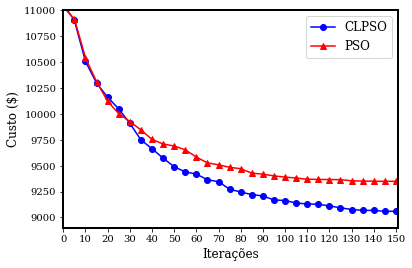
\includegraphics[width=100mm]{images/custo_medio_ieee30.png}
   
\fonte{Autor.}
\end{figure}

Nas Tabelas \ref{Pieee30} e \ref{Qieee30} estão os dados de potência ativa e reativa das melhores soluções factíveis de todos os métodos desenvolvidos no trabalho. 
O método híbrido proposto foi o que obteve maior sucesso na minimização indireta das perdas em relação aos demais métodos. Além disso, todas as potências encontradas estão fora das ZOP estabelecidas na Tabela \ref{ZOPieee30}. Pode-se observar também, através da Tabela \ref{Qieee30}, que as potências reativas encontradas por cada método encontram-se dentro dos limites estabelecidos pelos dados do sistema elétrico no Apêndice B.


\begin{table}[h!]
\centering
\caption{\label{Pieee30}Soluções de potência ativa obtidas pelos métodos PSO, SQP-BB, CLPSO e CLPSO-SQP-BB no sistema IEEE de 30 barras.}
\begin{tabular}{c c c c c}
	\hline
	\textbf{\makecell{Variável (MW)}} & \textbf{\makecell{PSO}} &
	\textbf{\makecell{SQP-BB}} &
	\textbf{\makecell{CLPSO}} &\textbf{\makecell{CLPSO-SQP-BB}}\\ 
	\hline

 \rule{0mm}{3ex} $P^G_1$& 182,4158 & 182,7554& 182,1720 & 182,3903\\[2mm]
$P^G_2$ & 34,9946 & 35,0000 & 35,3559& 35,0000 \\[2mm]
$P^G_5$ & 50,0021 &25,0000 & 50,0463 & 50,0000 \\[2mm]
$P^G_8$  & 25,0000	&25,0000 & 25,0000& 25,0000 \\[2mm]
$P^G_{11}$  & 0,0000 &25,0000 & 0,0000& 0,0000 \\[2mm]
$P^G_{13}$  & 0,0000 &0,0000 & 0,0029& 0,0000 \\[2mm]
Total  & 292,4125 & 292,7554& 292,5771& 292,3903 \\ [2mm]
Demanda & 283,4000 &283,4000 & 283,4000& 283,4000\\[2mm]
Perdas & 9,0125 & 9,3554 & 9,1771& 8,9903 \\[2mm]
\hline
\end{tabular}
\fonte{Autor.}
\end{table}


\begin{table}[h!]
\centering
\caption{\label{Qieee30}Soluções de potência reativa obtidas pelos métodos PSO, SQP-BB, CLPSO e CLPSO-SQP-BB no sistema IEEE de 30 barras.}
\begin{tabular}{c c c c c}
	\hline
	\textbf{\makecell{Variável (MVAr)}} & \textbf{\makecell{PSO}} &
	\textbf{\makecell{SQP-BB}} &
	\textbf{\makecell{CLPSO}} &\textbf{\makecell{CLPSO-SQP-BB}}\\ 
	\hline

 \rule{0mm}{3ex}
$Q^G_1 $ & 0,4666& 0,0000 &0,0000 & 0,0000 \\[2mm]
$Q^G_2$ &24,1610& 14,0351& 26,1401& 16,2514\\[2mm]
$Q^G_5$ &25,1220 & 28,4414& 23,9242	& 26,2711 \\[2mm]
$Q^G_8 $ & 39,7398& 40,0000	& 34,6769& 40,0000 \\[2mm]
$Q^G_{11}$ &14,2169& 18,7741& 15,9217& 17,6874\\[2mm]
$Q^G_{13}$ &18,8620& 23,2242& 19,0682& 23,4600\\[2mm]
\hline
\end{tabular}
\fonte{Autor.}
\end{table}

Na Tabela \ref{tebshieee30} estão os dados das variáveis discretas das melhores soluções de cada método. Nas Figuras \ref{ieee_30_volt} e \ref{ieee_30_ang} estão, respectivamente, os dados de manitude e ângulo de tensão das melhores soluções obtidas pelos métodos CLPSO e CLPSO-SQP-BB. Em relação ao caso anterior, nota-se uma maior divergência nos valores das magnitudes de tensões. De forma geral, para o sistema IEEE de 30 barras, o método híbrido proposto obteve resultados que também justificam sua superioridade em relação aos demais métodos. Obteve média e valor mínimo de custo menores que todos os demais métodos e a maior taxa de sucesso na obtenção de soluções factíveis. 

\begin{table}[h!]
\centering
\caption{\label{tebshieee30}Soluções de \emph{tap} e susceptância \emph{shunt}  obtidas pelos métodos PSO, SQP-BB, CLPSO e CLPSO-SQP-BB no sistema IEEE de 30 barras.}
\begin{tabular}{c c c c c}
	\hline
	\textbf{\makecell{Variável (\emph{pu})}} & \textbf{\makecell{PSO}} &
	\textbf{\makecell{SQP-BB}} &
	\textbf{\makecell{CLPSO}} &\textbf{\makecell{CLPSO-SQP-BB}}\\ 
	\hline

$t_{6,9}$ &1,00&1,03 &1,01& 1,02\\
$t_{6,10}$ &0,90&0,90 &0,99& 0,90\\
$t_{4,12}$ &0,98&1,00 &1,00& 1,00\\
$t_{28,27}$ &0,95&0,96 &0,95& 0,96\\
$b^{sh}_{10}$ &0,05&0,05&0,04& 0,05\\
$b^{sh}_{24}$ &0,05&0,05&0,05& 0,05\\
\hline
\end{tabular}
\fonte{Autor.}
\end{table}

\begin{figure}[h]
    \caption{\label{ieee_30_volt}Magnitudes de tensão obtidas pelos métodos CLPSO e CLPSO-SQP-BB no sistema IEEE de 30 barras.}
    \centering
    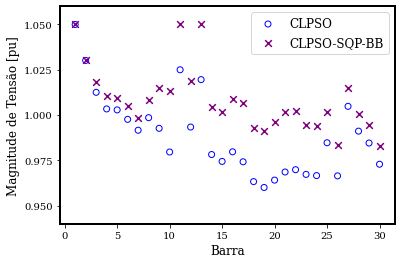
\includegraphics[width=100mm]{images/tensoes_ieee30.png}
   
\fonte{Autor.}
\end{figure}

\begin{figure}[h!]
    \caption{\label{ieee_30_ang}Ângulos de tensão obtidos pelos métodos CLPSO e CLPSO-SQP-BB no sistema IEEE de 30 barras}
    \centering
    \includegraphics[width=100mm]{images/ângulos_ieee30.png}
   
\fonte{Autor.}
\end{figure}


\section{Fluxo de Potência Ótimo Reativo}

No Apêndice C, são apresentados os dados dos sistemas IEEE de 118 e 300 barras. Para os casos testes do problema de FPOR, foram utilizadas as tolerâncias $\tau_p = 10^{-6}$ com $\tau_q = 10^{-6}$ para o método FD e $\tau_{opt} = 10^{-6}$ com $\tau_{fact} = 10^{-6}$ para o método SQP. Para execução do método BB, foi definida uma tolerância $\tau_{int} = 5\times10^{-5}$ de desvio para as variáveis discretas para uma solução ser considerada factível e foi utilizada a estratégia de busca adaptativa na exploração dos nós. Nas metaheurísticas, foram consideradas infactíveis soluções com ultrapassagens superiores a $10^{-6}$ dos limites das variáveis dependentes dos sistemas.

\subsection{Caso 1: Sistema Elétrico IEEE de 118 Barras}

O sistema IEEE de 118 barras tem os seguintes elementos:

\begin{itemize}
    \item 1 barra de geração \emph{slack};
    \item 53 barras de geração com controle de reativos;
    \item 64 barras de carga;
    \item 186 linhas de transmissão;
    \item 9 transformadores com \emph{tap} variável;
    \item 14 banco de capacitores ou reatores \emph{shunt} variável.
\end{itemize}


As perdas de potência ativa com os dados iniciais do sistema são de 132,8629 MW. Na modelagem, considerou-se que a magnitude de tensão nas barras tem como limites mínimos e máximos 0,94 e 1,06 \emph{pu}, respectivamente. Além disso, os \emph{taps} dos transformadores devem pertencer ao conjunto discreto \{0,90; 0,91; 0,92; 0,93; 0,94; 0,95; 0,96; 0,97; 0,98; 0,99; 1,0; 1,01; 1,02; 1,03; 1,04; 1,05; 1,06; 1,07; 1,08; 1,09; 1,1\} \emph{pu}. Já as susceptâncias \emph{shunt} dos bancos de capacitores ou reatores devem pertencer aos conjuntos discretos estabelecidos na Tabela \ref{tapseshunts118}. No trabalho de \citeonline{antlion} - um dos poucos a ter aplicado métodos metaheurísticos em sistemas elétricos de maior porte considerando a presença de variáveis discretas - os autores alteram os limites mínimos e máximos das potências reativas geradas pelos geradores do sistema para -500 MVAr e 500 MVAr, respectivamente. A mesma estratégia também é utilizada por \citeonline{IPGPSO}. 

Conforme será visto neste trabalho, a estratégia de ampliar os limites de geração de potência reativa dos geradores acaba favorecendo o funcionamento das metaheurísticas, uma vez que as penalizações de tais variáveis tornam-se menos relevantes na função \emph{fitness}. No entanto, a adoção de maiores limitantes acaba por gerar um cenário de operação pouco provável na prática. No trabalho proposto, serão avaliados dois casos distintos: no primeiro, serão adotados os mesmos limites de geração de potência reativa que os utilizados por \citeonline{antlion} e \citeonline{IPGPSO}; no segundo, serão adotados os limites do banco de dados do pacote \emph{pandapower}.

\begin{table}[h!]
\centering
\caption{\label{tapseshunts118}Susceptâncias dos bancos de capacitores e reatores \emph{shunt} do sistema elétrico IEEE de 118 barras.}
\begin{tabular}{c c c c}
	\hline
	\textbf{\makecell{Variável}} & 
	\textbf{\makecell{Valor \\ Mínimo}} &
	\textbf{\makecell{Valor \\ Máximo}} &
	\textbf{\makecell{Passo\\Discreto}} \\ 
	\hline

$b^{sh}_{5}$ &-0,40&0,00 &0,01\\
$b^{sh}_{34}$ &0,00&0,14 &0,01\\
$b^{sh}_{37}$ &-0,25&0,00 &0,01\\
$b^{sh}_{44}$ &0,00&0,10 &0,01\\
$b^{sh}_{45}$ &0,00&0,10 &0,01\\
$b^{sh}_{46}$ &0,00&0,10 &0,01\\
$b^{sh}_{48}$ &0,00&0,15 &0,01\\
$b^{sh}_{74}$ &0,00&0,12 &0,01\\
$b^{sh}_{79}$ &0,00&0,20 &0,01\\
$b^{sh}_{82}$ &0,00&0,20 &0,01\\
$b^{sh}_{83}$ &0,00&0,10 &0,01\\
$b^{sh}_{105}$ &0,00&0,20 &0,01\\
$b^{sh}_{107}$ &0,00&0,06 &0,01\\
$b^{sh}_{110}$ &0,00&0,06 &0,01\\
\hline
\end{tabular}
\fonte{\citeonline{antlion}}
\end{table}


Os resultados obtidos pelo método híbrido serão comparados aos dos métodos: SQP-BB, PSO, CLPSO, otimizador formiga-leão (do inglês \emph{ant lion optimizer} ou ALO), GWO e algoritmo de colônia de abelhas artificiais (do inglês \emph{artificial bee colony algorithm} ou ABC). Os métodos ALO, GWO e ABC foram desenvolvidos por \citeonline{antlion}, utilizando os mesmos dados do sistema elétrico e considerando os mesmos valores de \emph{taps} e susceptâncias \emph{shunt}. 

No primeiro caso, para as metaheurísticas PSO e CLPSO, foram utilizados enxames de 40 partículas com 100 iterações e peso de inércia linearmente decrescente. Já no segundo caso, foram utilizados enxames de 40 partículas com 250 iterações e peso de inércia linearmente decrescente. Os dados dos hiperparâmetros encontram-se na Tabela \ref{configieee1181}. No método híbrido, após encontrar as soluções pelo método CLPSO, os conjuntos de variáveis discretas foram reduzidos aos 2 vizinhos imediatamente inferiores e superiores possíveis para os \emph{taps} e \emph{shunts} de $g^{best}$, a fim de executar o método SQP-BB. Ao todo, foram realizadas 25 execuções dos métodos PSO, CLPSO e CLPSO-SQP-BB para mensurar seus respectivos desempenhos. Para o método determinístico SQP-BB, foi realizada a execução partindo do ponto inicial do banco de dados.

\begin{table}[h]
\centering
\caption{\label{configieee1181} Hiperparâmetros das metaheurísticas PSO e CLPSO.}

\begin{tabular}{c c c c c c c c c c c c}
	\hline
    Método & $c_1$ & $c_2$ & $c$ & $w^{min}$ & $w^{max}$ & $r^{gap}$ & $p_t$ & \mu& \beta & $\zeta$ & $\omega$ \\
    
    PSO (caso 1) & 2 & 2 & - & 0,4 & 0,9 & - & - & 0,1& 0,1 & $10^3$ & $10^3$ \\

    PSO (caso 2) & 2 & 2 & - & 0,4 & 0,9 & - & - & 0,1& 0,1 & $1$ & $5\times10^{-2}$ \\
    
    CLPSO (caso 1) & - & - & 1 & 0,4  & 0,9 & 0 & 0,9 &  0,1 & 0,1  & $10^3$ & $10^3$ \\    

    CLPSO (caso 2) & - & - & 1 & 0,4  & 0,9 & 0 & 0,9 &  0,1 & 0,1  & $1$ & $5\times10^{-2}$ \\    
    
    \hline
\end{tabular}
\fonte{Autor.}
\end{table}

Na Tabela \ref{resultsieee1181} estão os resultados obtidos pelos algoritmos CLPSO, PSO, ALO, GWO, ABC e CLPSO-SQP-BB, apenas para as soluções factíveis. Já na Tabela \ref{timesieee1181} estão os dados de tempo de execução, número de agentes de busca e iterações reportados pelos autores de cada método.

\begin{table}[h]
\centering
\caption{\label{resultsieee1181}Valores mínimos, médios e desvios padrão obtidos para a função perdas do problema de FPOR no sistema IEEE de 118 barras.}

\begin{tabular}{c c c c}
	\hline
	\textbf{\makecell{Método}} & \textbf{\makecell{Perda \\ Mínima (MW)}} &
	\textbf{\makecell{Perda\\Média (MW)}} & \textbf{\makecell{Desvio\\Padrão (MW)}} \\
	\hline

    \makecell{GWO\\
	\tiny\cite{antlion}} &  \makecell{131,2620}   & \makecell{-}  & -   \\
    \makecell{ABC\\
	\tiny\cite{antlion}} &  \makecell{120,4288}   & \makecell{-}  & -   \\
	
	\makecell{ALO\\
	\tiny\cite{antlion}} &  \makecell{119,7792}   & \makecell{-}  & -  \\

	\makecell{SQP-BB (caso 1)} &  \makecell{114,2876}   & \makecell{-}  & \makecell{-} \\
	
	\makecell{SQP-BB (caso 2)} &  \makecell{-}   & \makecell{-}  & \makecell{-} \\
	
	\makecell{PSO (caso 1)} &  \makecell{121,2664}   & \makecell{123,1461}  & \makecell{1,2349} \\
	
	\makecell{PSO (caso 2)} &  \makecell{-}   & \makecell{-}  & \makecell{-} \\

	\makecell{CLPSO (caso 1)} &  \makecell{117,7210}   & \makecell{118,9979}  & \makecell{0,5482} \\
	
	\makecell{CLPSO (caso 2)} &  \makecell{120,3600}   & \makecell{121,1000}  & \makecell{0,4700} \\
	
	\makecell{\textbf{CLPSO-SQP-BB (caso 1)}} &  \makecell{\textbf{114,3810}}   & \makecell{\textbf{115,4540}}  &  \textbf{1,8707}  \\
	
	\makecell{\textbf{CLPSO-SQP-BB (caso 2)}} &  \makecell{\textbf{115,1109}}   & \makecell{\textbf{115,8182}}  &  \textbf{1,603}  \\
	\hline
\end{tabular}
\fonte{Autor.}
\end{table}

Para o caso 1, todos os algoritmos desenvolvidos no trabalho apresentaram 100\% de sucesso na obtenção de soluções factíveis. No caso 2, os métodos PSO e SQP-BB não conseguiram obter uma solução factível para o problema, e os métodos CLPSO e CLPSO-SQP-BB apresentaram, respectivamente, taxas de sucesso de 56\% e 84\%. Vale destacar o desempenho da metaheurística CLPSO que obteve bons resultados até mesmo para o caso que considera os limites originais do banco de dados do sistema para as potências reativas geradas. 

Analisando-se a Tabela \ref{timesieee118}, pode-se observar que os métodos programados por \citeonline{antlion} tendem a gastar um elevado tempo de execução em comparação aos métodos desenvolvidos neste trabalho. Ainda, vale ressaltar o tempo obtido pelo método SQP-BB no caso 1, maior que o obtido pelas metaheurísticas e pelo método híbrido. Neste caso, o elevado tempo de execução tem relaçao com o grande número de variáveis discretas do problema, o que gera uma grande quantidade de nós a serem ramificados e explorados no processo de otimização. Neste sentido, a estratégia de limitar a vizinhança das variáveis discretas ao redor da solução $g^{best}$ ajuda a minimizar a quantidade de nós a serem explorados, garantindo um menor tempo de execução sem afetar significativamente a qualidade das soluções em relação ao caso de vizinhança ilimitada.

\begin{table}[h]
\centering
\caption{\label{timesieee118}Dados das performances dos métodos no sistema IEEE de 118 barras.}
\begin{tabular}{c c c c c}
	\hline
	\textbf{\makecell{Método}} & \textbf{\makecell{Tempo \\Médio(s)}} &
	\textbf{\makecell{Desvio \\Padrão(s)}} &
	\textbf{\makecell{Nº de\\ Agentes}} &
	\textbf{\makecell{Nº de \\Iterações}} &
	
	\hline

    \makecell{ABC\\
	\tiny\cite{antlion}} &  \makecell{730,40}   & -& \makecell{40}  & 100   \\
	
    \makecell{GWO\\
	\tiny\cite{antlion}} &  \makecell{722,45}   &- & \makecell{40}  & 100   \\

	\makecell{ALO\\
	\tiny\cite{antlion}} &  \makecell{716,76}   &  - & \makecell{40} &100  \\
	
	\makecell{SQP-BB (caso 1)} &  \makecell{434,31}   & \makecell{-}  & -& \makecell{100} \\
	
	\makecell{SQP-BB (caso 2)} &  \makecell{-}   & \makecell{-}  & -& \makecell{-} \\
	\makecell{PSO (caso 1)} &  \makecell{123,78}   & \makecell{11,98}  & 40& \makecell{100} \\
	
	\makecell{PSO (caso 2)} &  \makecell{268,14}   & \makecell{13,07}  & 40& \makecell{250} \\
	
	\makecell{CLPSO (caso 1)} &  \makecell{107,76}   & \makecell{5,57}  & \makecell{40} & \makecell{100} \\
	
	
	\makecell{CLPSO (caso 2)} &  \makecell{268,77}   & \makecell{21,73}  & \makecell{40} & \makecell{250} \\
	
	\makecell{\textbf{CLPSO-SQP-BB (caso 1)}} &  \makecell{\textbf{128,45}}   & \makecell{\textbf{29,27}}  &  \textbf{-}  & \textbf{248}\tablefootnote[8]{Número médio de iterações para o método híbrido no sistema IEEE de 118 barras (caso 1).}  \\
	
	
	\makecell{\textbf{CLPSO-SQP-BB (caso 2)}} &  \makecell{\textbf{274,52}}   & \makecell{\textbf{26,15}}  &  \textbf{-}  & \textbf{276}\tablefootnote[9]{Número médio de iterações para o método híbrido no sistema IEEE de 118 barras (caso 2).}  \\
	\hline
\end{tabular}
\fonte{Autor.}
\end{table}


A Figura \ref{ieee_1181_curves} ilustra os valores médios da função objetivo da partícula $g^{best}$ em cada uma das iterações das execuções das metaheurísticas PSO e CLPSO que obtiveram soluções factíveis no caso 1. Pode-se observar que a partir da iteração de número 20, o método CLPSO tende a continuar melhorando a função objetivo do problema de forma mais acentuada que o algoritmo PSO. Nas Figuras \ref{tensao11812} e \ref{angulo11812}, podem ser visualizados os valores de manigutes e ângulos de tensão obtidos pelo método híbrido em ambos os casos. Ainda, nas Figuras \ref{trafos11812} e \ref{tapseshunts118} estão os valores obtidos de \emph{taps} e susceptâncias \emph{shunt}. Todas as variáveis do problema encontram-se dentro dos limites especificados no trabalho, assim como as variáveis discretas pertencem aos conjuntos de valores discretos estabelecidos no início desta subseção.

\pagebreak

\begin{figure}[h!]
    \caption{\label{ieee_1181_curves}Média das curvas de convergência para as metaheurísticas PSO e CLPSO no sistema IEEE de 118 barras para o caso 1.}
    \centering
    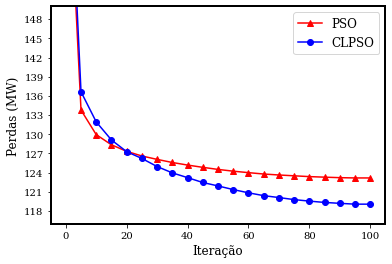
\includegraphics[width=100mm]{images/convergence_curves_ieee118_1.png}
   
\fonte{Autor.}
\end{figure}

\begin{figure}[h!]
    \caption{\label{tensao11812}Magnitudes de tensão obtidas pelo método CLPSO-SQP-BB nos casos 1 e 2.}
    \centering
    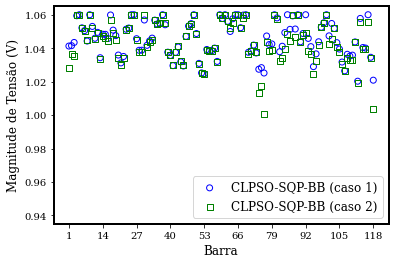
\includegraphics[width=100mm]{images/tensao_ieee118_hibrido.png}
   
\fonte{Autor.}
\end{figure}

\pagebreak

\begin{figure}[h!]
    \caption{\label{angulo11812}Ângulos de tensão obtidos pelo método CLPSO-SQP-BB nos casos 1 e 2.}
    \centering
    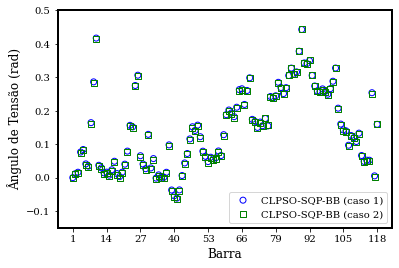
\includegraphics[width=100mm]{images/angulo_ieee118_hibrido.png}
   
\fonte{Autor.}
\end{figure}


\begin{figure}[h!]
    \caption{\label{trafos11812}\emph{Taps} obtidos pelo método CLPSO-SQP-BB nos casos 1 e 2.}
    \centering
    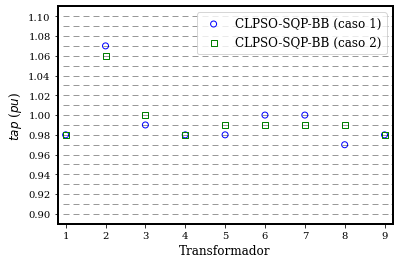
\includegraphics[width=100mm]{images/trafos_ieee118_hibrido.png}
   
\fonte{Autor.}
\end{figure}

\pagebreak

\begin{figure}[h!]
    \caption{\label{shunts11812}Susceptâncias \emph{shunt} obtidas pelo método CLPSO-SQP-BB nos casos 1 e 2.}
    \centering
    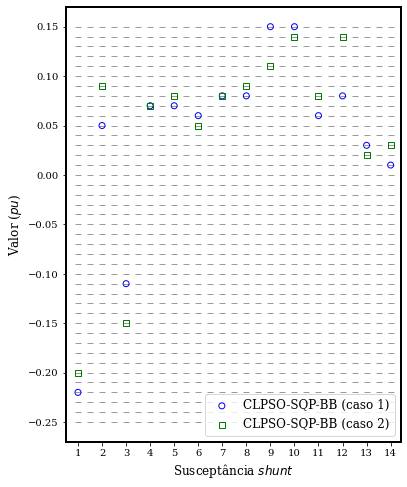
\includegraphics[width=100mm]{images/shunt_ieee118.png}
   
\fonte{Autor.}
\end{figure}


Novamente, o método híbrido desenvolvido apresentou performance superior aos demais métodos utilizados na comparação deste trabalho. No caso 1, embora não tenha conseguido obter soluções melhores que a do método SQP-BB, acabou apresentando tempo de execução consideravelmente menor. No caso 2, além da boa performance do método híbrido, vale ressaltar a capacidade da metaheurística CLPSO em resolver o problema de grande dimensão considerando também a presença de variáveis discretas. O algoritmo PSO, por exemplo, foi incapaz de encontrar soluções factíveis neste caso. Além disso, o método SQP-BB também não conseguiu resolver o problema partindo dos dados iniciais do banco de dados. Portanto, fica evidente que a estratégia de aprendizagem abrangente também traz benefícios quando utilizada em problemas de grandes dimensões, mesmo que não sejam do tipo multimodal.

\subsection{Caso 2: Sistema Elétrico IEEE de 300 Barras}



O sistema IEEE de 300 barras tem os seguintes elementos:

\begin{itemize}
    \item 1 barra de geração \emph{slack};
    \item 68 barras de geração com controle de reativos;
    \item 231 barras de carga;
    \item 411 linhas de transmissão;
    \item 107 transformadores com \emph{tap} variável;
    \item 14 banco de capacitores ou reatores \emph{shunt} variável.
\end{itemize}


As perdas de potência ativa com os dados iniciais do sistema são de 408,3160 MW. Na modelagem, considerou-se que a magnitude de tensão nas barras tem como limites mínimos e máximos 0,90 e 1,10 \emph{pu}, respectivamente. Além disso, os \emph{taps} dos transformadores devem pertencer ao conjunto discreto \{0,90; 0,91; 0,92; 0,93; 0,94; 0,95; 0,96; 0,97; 0,98; 0,99; 1,0; 1,01; 1,02; 1,03; 1,04; 1,05; 1,06; 1,07; 1,08; 1,09; 1,1\} \emph{pu} \cite{antlion}. Já as susceptâncias \emph{shunt} dos bancos de capacitores ou reatores devem pertencer aos conjuntos discretos estabelecidos na Tabela \ref{tapseshunts300}.


\begin{table}[h!]
\centering
\caption{\label{tapseshunts300}Susceptâncias dos bancos de capacitores e reatores \emph{shunt} do sistema elétrico IEEE de 300 barras.}
\begin{tabular}{c c c c}
	\hline
	\textbf{\makecell{Variável}} & 
	\textbf{\makecell{Valor \\ Mínimo}} &
	\textbf{\makecell{Valor \\ Máximo}} &
	\textbf{\makecell{Passo\\Discreto}} \\ 
	\hline

$b^{sh}_{96}$ &0,00&4,50 &0,01\\
$b^{sh}_{99}$ &0,00&0,59 &0,01\\
$b^{sh}_{133}$ &0,00&0,39 &0,01\\
$b^{sh}_{143}$ &-4,50&0,00 &0,01\\
$b^{sh}_{145}$ &-4,50&0,00 &0,01\\
$b^{sh}_{152}$ &0,00&0,59 &0,01\\
$b^{sh}_{158}$ &0,00&0,59 &0,01\\
$b^{sh}_{169}$ &-2,50&0,00 &0,01\\
$b^{sh}_{210}$ &-4,50&0,00 &0,01\\
$b^{sh}_{217}$ &-4,50&0,00 &0,01\\
$b^{sh}_{219}$ &-1,50&0,00 &0,01\\
$b^{sh}_{227}$ &0,00&0,59 &0,01\\
$b^{sh}_{268}$ &0,00&0,15 &0,01\\
$b^{sh}_{283}$ &0,00&0,15 &0,01\\
\hline
\end{tabular}
\fonte{\citeonline{antlion}}
\end{table}


\chapter{Conclusão}
% ---

\lipsum[31-33]

% ----------------------------------------------------------
% ELEMENTOS PÓS-TEXTUAIS
% ----------------------------------------------------------
\postextual
% ----------------------------------------------------------

% ----------------------------------------------------------
% Referências bibliográficas
% ----------------------------------------------------------
\bibliography{references}

% ----------------------------------------------------------
% Glossário
% ----------------------------------------------------------
%
% Consulte o manual da classe abntex2 para orientações sobre o glossário.
%
%\glossary

% ----------------------------------------------------------
% Apêndices
% ----------------------------------------------------------

% ---
% Inicia os apêndices
% ---
\begin{apendicesenv}

% Imprime uma página indicando o início dos apêndices
\partapendices

% ----------------------------------------------------------
\chapter{Dados dos Problemas de Despacho Econômico com Ponto de Carregamento de Válvula}
% ----------------------------------------------------------


\section{Caso 1: 13 Unidades Geradoras}

Os dados dos coeficientes da função custo e dos limites de geração de potência ativa das unidades geradoras encontram-se na Tabela \ref{13coef}.

\begin{table}[h]
\caption{\label{13coef}Dados para o caso 1 (Demanda: $P^D=2520$ MW).}
\center
\begin{tabular}{c c c c c c c c}
\hline
 $k$  & $a_k$       & $b_k$    & $c_k$     & $e_k$     & $f_k$     & $\underline{P^G_k}$ (MW)    & $\overline{P^G_k} $(MW)  \\
 \hline
1  & 0,00028 & 8,1  & 550,0 & 300,0 & 0,035 & 0,0  & 680,0 \\
2  & 0,00056 & 8,1  & 309,0 & 200,0 & 0,042 & 0,0  & 360,0 \\
3  & 0,00056 & 8,1  & 307,0 & 200,0 & 0,042 & 0,0  & 360,0 \\
4  & 0,00324 & 7,74 & 240,0 & 150,0 & 0,063 & 60,0 & 180,0 \\
5  & 0,00324 & 7,74 & 240,0 & 150,0 & 0,063 & 60,0 & 180,0 \\
6  & 0,00324 & 7,74 & 240,0 & 150,0 & 0,063 & 60,0 & 180,0 \\
7  & 0,00324 & 7,74 & 240,0 & 150,0 & 0,063 & 60,0 & 180,0 \\
8  & 0,00324 & 7,74 & 240,0 & 150,0 & 0,063 & 60,0 & 180,0 \\
9  & 0,00324 & 7,74 & 240,0 & 150,0 & 0,063 & 60,0 & 180,0 \\
10  & 0,00284 & 8,6  & 126,0 & 100,0 & 0,084 & 40,0 & 120,0 \\
11 & 0,00284 & 8,6  & 126,0 & 100,0 & 0,084 & 40,0 & 120,0 \\
12 & 0,00284 & 8,6  & 126,0 & 100,0 & 0,084 & 55,0 & 120,0 \\
13 & 0,00284 & 8,6  & 126,0 & 100,0 & 0,084 & 55,0 & 120,0\\
\hline
\end{tabular}
\fonte{\citeonline{dados13}}
\end{table}


Para definir os hiperparâmetros $c$, $p_t$ e $r^{gap}$ da metaheurística CLPSO, foram realizados 15 execuções do método para o problema em questão e calculados os valores médios e desvios padrão. Os parâmetros $c$ e $r^{gap}$ foram variados em passos unitários no intervalo de 1 a 3 e 0 a 3, respectivamente. Já $p_t$ foi variado em passos discretos de 0,1 no intervalo de 0,1 a 0,9. Os gráficos de barra de erro abaixo ilustram os valores médios centralizados nas barras de dispersão que possuem tamanho de 1 desvio padrão para mais e para menos. A melhor configuração para o caso teste de 13 unidades geradoras foi: $r_gap=0$, $c=1$ e $p_t=0,4$, com custo médio de 24234,3010 \$ e desvio padrão de 54,3240 \$.

\begin{figure}[h!]
    \caption{\label{rgap0_13}Configurações de $c$ e $p_t$ para $r^{gap}=0$ (caso 1).}
    \centering
    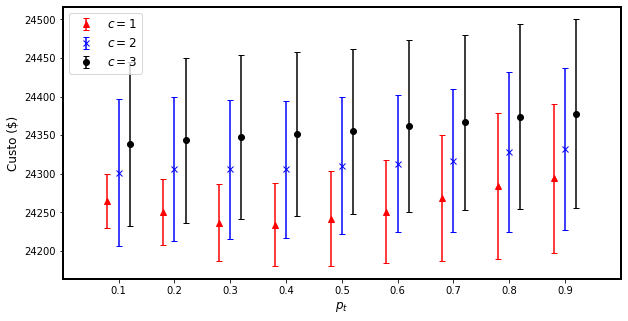
\includegraphics[width=120mm, height=60mm]{images/rgap0_13.png}
   
\fonte{Autor.}
\end{figure}

\begin{figure} [h!]
    \centering
    \caption{\label{rgap1_13}Configurações de $c$ e $p_t$ para $r^{gap}=1$ (caso 1).}
    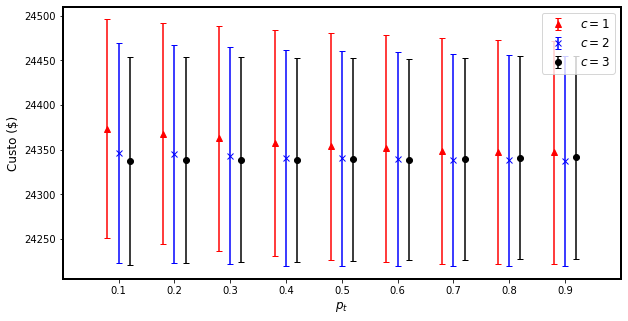
\includegraphics[width=120mm, height=60mm]{images/rgap1_13.png}
    \fonte{Autor.}
\end{figure}


\begin{figure}[h!]
    \caption{\label{rgap2_13}Configurações de $c$ e $p_t$ para $r^{gap}=2$ (caso 1).}
    \centering
    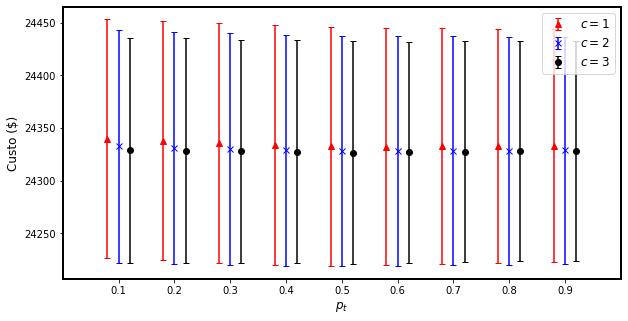
\includegraphics[width=120mm, height=60mm]{images/rgap2_13.png}

\fonte{Autor.}
\end{figure}

\begin{figure}[h!]
    \caption{\label{rgap3_13}Configurações de $c$ e $p_t$ para $r^{gap}=3$ (caso 1).}
    \centering
    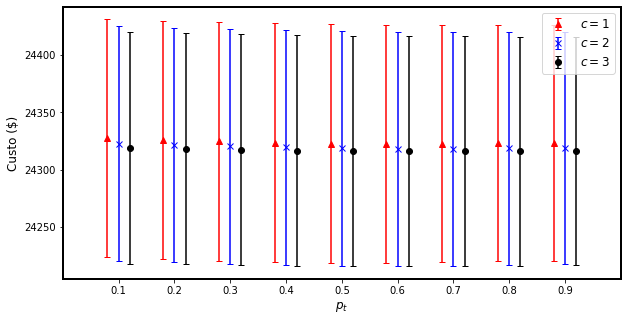
\includegraphics[width=120mm, height=60mm]{images/rgap3_13.png}
    \fonte{Autor.}
\end{figure}



\pagebreak
\section{Caso 2: 19 Unidades Geradoras}

Os dados dos coeficientes da função custo e dos limites de geração de potência ativa das unidades geradoras encontram-se na Tabela \ref{19coef}.

\begin{table}[h]
\caption{\label{19coef}Dados para o caso 2 (Demanda: $P^D=2908$ MW).}
\center
\begin{tabular}{c c c c c c c c}
\hline
 $k$  & $a_k$       & $b_k$    & $c_k$     & $e_k$     & $f_k$     & $\underline{P^G_k}$ (MW)    & $\overline{P^G_k} $(MW)  \\
 \hline
1  & 0,0097 & 6,8   & 119,0 & 90,0 & 0,72 & 100,0 & 300,0 \\
2  & 0,0055 & 4,0   & 90,0  & 79,0 & 0,05 & 120,0 & 438,0 \\
3  & 0,0055 & 4,0   & 45,0  & 0,0  & 0,0  & 100,0 & 250,0 \\
4  & 0,0025 & 0,85  & 0,0   & 0,0  & 0,0  & 8,0   & 25,0  \\
5  & 0,0    & 5,28  & 0,891 & 0,0  & 0,0  & 50,0  & 63,75 \\
6  & 0,008  & 3,5   & 110,0 & 0,0  & 0,0  & 150,0 & 300,0 \\
7  & 0,0    & 5,439 & 21,0  & 0,0  & 0,0  & 50,0  & 63,75 \\
8  & 0,0075 & 6,0   & 88,0  & 50,0 & 0,52 & 100,0 & 500,0 \\
9  & 0,0085 & 6,0   & 55,0  & 0,0  & 0,0  & 200,0 & 600,0 \\
10  & 0,009  & 5,2   & 90,0  & 0,0  & 0,0  & 15,0  & 40,0  \\
11 & 0,0045 & 1,6   & 65,0  & 0,0  & 0,0  & 50,0  & 150,0 \\
12 & 0,0025 & 0,85  & 78,0  & 58,0 & 0,02 & 25,0  & 75,0  \\
13 & 0,0    & 2,55  & 49,0  & 0,0  & 0,0  & 50,0  & 63,75 \\
14 & 0,0045 & 1,6   & 85,0  & 0,0  & 0,0  & 0,0   & 95,0  \\
15 & 0,0065 & 4,7   & 80,0  & 92,0 & 0,75 & 20,0  & 220,0 \\
16 & 0,0045 & 1,4   & 90,0  & 0,0  & 0,0  & 15,0  & 80,0  \\
17 & 0,0025 & 0,85  & 10,0  & 0,0  & 0,0  & 15,0  & 80,0  \\
18 & 0,0045 & 1,6   & 25,0  & 0,0  & 0,0  & 50,0  & 230,0 \\
19 & 0,008  & 5,5   & 90,0  & 0,0  & 0,0  & 400,0 & 500,0\\
\hline
\end{tabular}
\fonte{\citeonline{balamurugan}}
\end{table}


Para definir os hiperparâmetros $c$, $p_t$ e $r^{gap}$ da metaheurística CLPSO, foram realizados 15 execuções do método para o problema em questão e calculados os valores médios e desvios padrão. Os parâmetros $c$ e $r^{gap}$ foram variados em passos unitários no intervalo de 1 a 3 e 0 a 3, respectivamente. Já $p_t$ foi variado em passos discretos de 0,1 no intervalo de 0,1 a 0,9. Os gráficos de barra de erro abaixo ilustram os valores médios centralizados nas barras de dispersão que possuem tamanho de 1 desvio padrão para mais e para menos. A melhor configuração para o caso teste de 19 unidades geradoras foi: $r_gap=3$, $c=3$ e $p_t=0,9$, com custo médio de 16983,4578 \$ e desvio padrão de 28,5936 \$.

\begin{figure}[h!]
    \caption{\label{rgap0_19}Configurações de $c$ e $p_t$ para $r^{gap}=0$ (caso 2).}
    \centering
    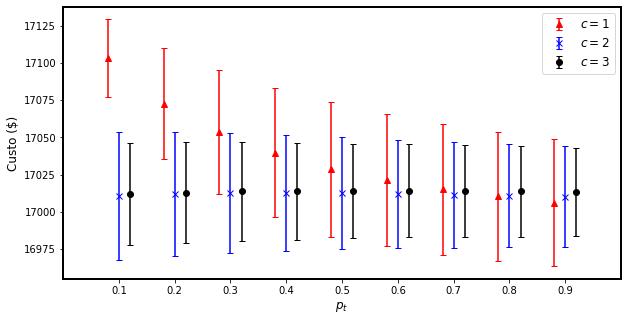
\includegraphics[width=120mm, height=60mm]{images/rgap0_19.png}
   
\fonte{Autor.}
\end{figure}

\begin{figure} [h!]
    \centering
    \caption{\label{rgap1_19}Configurações de $c$ e $p_t$ para $r^{gap}=1$ (caso 2).}
    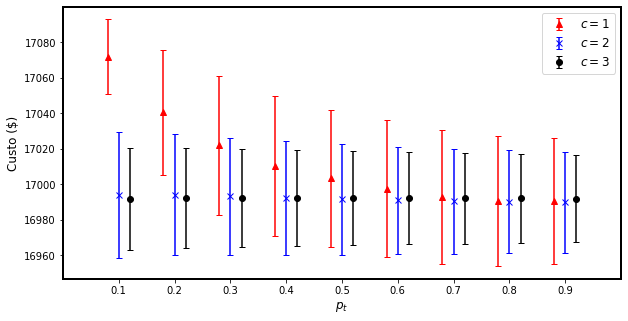
\includegraphics[width=120mm, height=60mm]{images/rgap1_19.png}
    \fonte{Autor.}
\end{figure}


\begin{figure}[h!]
    \caption{\label{rgap2_19}Configurações de $c$ e $p_t$ para $r^{gap}=2$ (caso 2).}
    \centering
    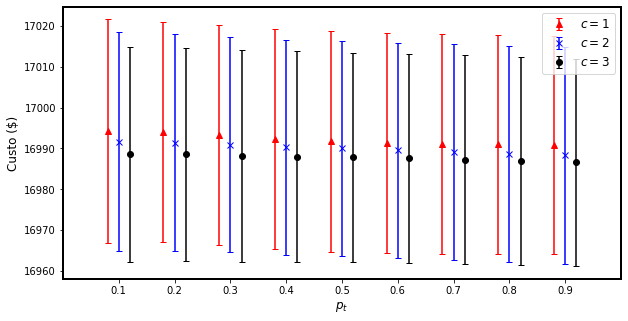
\includegraphics[width=120mm, height=60mm]{images/rgap2_19.png}

\fonte{Autor.}
\end{figure}

\begin{figure}[h!]
    \caption{\label{rgap3_19}Configurações de $c$ e $p_t$ para $r^{gap}=3$ (caso 2).}
    \centering
    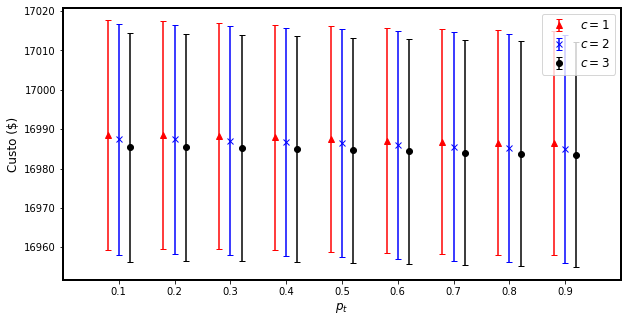
\includegraphics[width=120mm, height=60mm]{images/rgap3_19.png}
    \fonte{Autor.}
\end{figure}


\pagebreak
\\

\section{Caso 3: 40 Unidades Geradoras}

Os dados dos coeficientes da função custo e dos limites de geração de potência ativa das unidades geradoras encontram-se na Tabela \ref{40coef}. Para definir os hiperparâmetros $c$, $p_t$ e $r^{gap}$ da metaheurística CLPSO, foram realizados 15 execuções do método para o problema em questão e calculados os valores médios e desvios padrão. Os parâmetros $c$ e $r^{gap}$ foram variados em passos unitários no intervalo de 1 a 3 e 0 a 3, respectivamente. Já $p_t$ foi variado em passos discretos de 0,1 no intervalo de 0,1 a 0,9. Os gráficos de barra de erro abaixo ilustram os valores médios centralizados nas barras de dispersão que possuem tamanho de 1 desvio padrão para mais e para menos. A melhor configuração para o caso teste de 40 unidades geradoras foi: $r_gap=0$, $c=1$ e $p_t=0,9$, com custo médio de 121612,9850 \$ e desvio padrão de 191,0481 \$.


\begin{table}[h!]
\caption{\label{40coef}Dados para o caso 3 (Demanda: $P^D=10500$ MW).}
\center
\begin{tabular}{c c c c c c c c}
\hline
 $k$  & $a_k$       & $b_k$    & $c_k$     & $e_k$     & $f_k$     & $\underline{P^G_k}$ (MW)    & $\overline{P^G_k} $(MW)  \\
 \hline
1  & 0.0069  & 6.73 & 94.705 & 100.0 & 0.084 & 36.0  & 114.0 \\
2  & 0.0069  & 6.73 & 94.705 & 100.0 & 0.084 & 36.0  & 114.0 \\
3  & 0.02028 & 7.07 & 309.54 & 100.0 & 0.084 & 60.0  & 120.0 \\
4  & 0.00942 & 8.18 & 369.03 & 150.0 & 0.063 & 80.0  & 190.0 \\
5  & 0.0114  & 5.35 & 148.89 & 120.0 & 0.077 & 47.0  & 97.0  \\
6  & 0.01142 & 8.05 & 222.33 & 100.0 & 0.084 & 68.0  & 140.0 \\
7  & 0.00357 & 8.03 & 287.71 & 200.0 & 0.042 & 110.0 & 300.0 \\
8  & 0.00492 & 6.99 & 391.98 & 200.0 & 0.042 & 135.0 & 300.0 \\
9  & 0.00573 & 6.6  & 455.76 & 200.0 & 0.042 & 135.0 & 300.0 \\
10  & 0.00605 & 12.9 & 722.82 & 200.0 & 0.042 & 130.0 & 300.0 \\
11 & 0.00515 & 12.9 & 635.2  & 200.0 & 0.042 & 94.0  & 375.0 \\
12 & 0.00569 & 12.8 & 654.69 & 200.0 & 0.042 & 94.0  & 375.0 \\
13 & 0.00421 & 12.5 & 913.4  & 300.0 & 0.035 & 125.0 & 500.0 \\
14 & 0.00752 & 8.84 & 1760.4 & 300.0 & 0.035 & 125.0 & 500.0 \\
15 & 0.00708 & 9.15 & 1728.3 & 300.0 & 0.035 & 125.0 & 500.0 \\
16 & 0.00708 & 9.15 & 1728.3 & 300.0 & 0.035 & 125.0 & 500.0 \\
17 & 0.00313 & 7.97 & 647.85 & 300.0 & 0.035 & 220.0 & 500.0 \\
18 & 0.00313 & 7.95 & 649.69 & 300.0 & 0.035 & 220.0 & 500.0 \\
19 & 0.00313 & 7.97 & 647.83 & 300.0 & 0.035 & 242.0 & 550.0 \\
20 & 0.00313 & 7.97 & 647.81 & 300.0 & 0.035 & 242.0 & 550.0 \\
21 & 0.00298 & 6.63 & 785.96 & 300.0 & 0.035 & 254.0 & 550.0 \\
22 & 0.00298 & 6.63 & 785.96 & 300.0 & 0.035 & 254.0 & 550.0 \\
23 & 0.00284 & 6.66 & 794.53 & 300.0 & 0.035 & 254.0 & 550.0 \\
24 & 0.00284 & 6.66 & 794.53 & 300.0 & 0.035 & 254.0 & 550.0 \\
25 & 0.00277 & 7.1  & 801.32 & 300.0 & 0.035 & 254.0 & 550.0 \\
26 & 0.00277 & 7.1  & 801.32 & 300.0 & 0.035 & 254.0 & 550.0 \\
27 & 0.52124 & 3.33 & 1055.1 & 120.0 & 0.077 & 10.0  & 150.0 \\
28 & 0.52124 & 3.33 & 1055.1 & 120.0 & 0.077 & 10.0  & 150.0 \\
29 & 0.52124 & 3.33 & 1055.1 & 120.0 & 0.077 & 10.0  & 150.0 \\
30 & 0.0114  & 5.35 & 148.89 & 120.0 & 0.077 & 47.0  & 97.0  \\
31 & 0.0016  & 6.43 & 222.92 & 150.0 & 0.063 & 60.0  & 190.0 \\
33 & 0.0016  & 6.43 & 222.92 & 150.0 & 0.063 & 60.0  & 190.0 \\
33 & 0.0016  & 6.43 & 222.92 & 150.0 & 0.063 & 60.0  & 190.0 \\
34 & 0.0001  & 8.95 & 107.87 & 200.0 & 0.042 & 90.0  & 200.0 \\
35 & 0.0001  & 8.62 & 116.58 & 200.0 & 0.042 & 90.0  & 200.0 \\
36 & 0.0001  & 8.62 & 116.58 & 200.0 & 0.042 & 90.0  & 200.0 \\
37 & 0.0161  & 5.88 & 307.45 & 80.0  & 0.098 & 25.0  & 110.0 \\
38 & 0.0161  & 5.88 & 307.45 & 80.0  & 0.098 & 25.0  & 110.0 \\
39 & 0.0161  & 5.88 & 307.45 & 80.0  & 0.098 & 25.0  & 110.0 \\
40 & 0.00313 & 7.97 & 647.83 & 300.0 & 0.035 & 242.0 & 550.0\\
\hline
\end{tabular}
\small\fonte{\citeonline{dados13}}
\end{table}


\begin{figure}[h]
    \caption{\label{rgap0_40}Configurações de $c$ e $p_t$ para $r^{gap}=0$ (caso 3).}
    \centering
    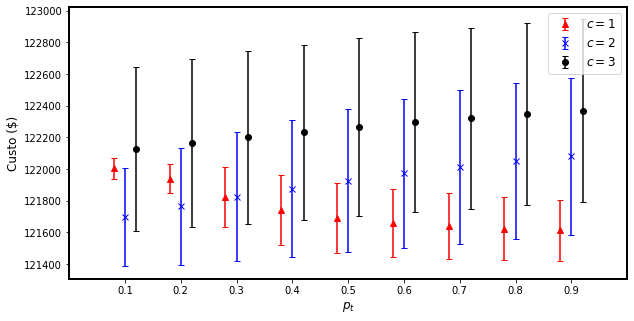
\includegraphics[width=120mm, height=60mm]{images/rgap0_40.png}
   
\fonte{Autor.}
\end{figure}

\begin{figure} [h]
    \centering
    \caption{\label{rgap1_40}Configurações de $c$ e $p_t$ para $r^{gap}=1$ (caso 3).}
    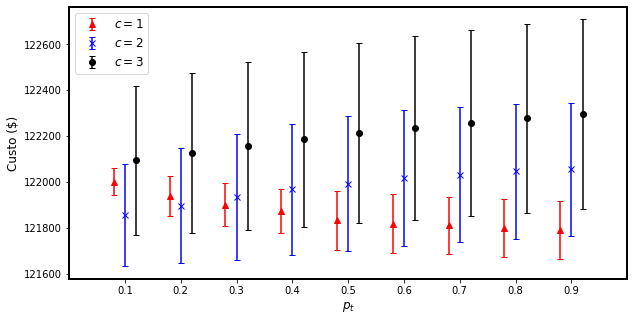
\includegraphics[width=120mm, height=60mm]{images/rgap1_40.png}
    \fonte{Autor.}
\end{figure}


\begin{figure}[h]
    \caption{\label{rgap2_40}Configurações de $c$ e $p_t$ para $r^{gap}=2$ (caso 3).}
    \centering
    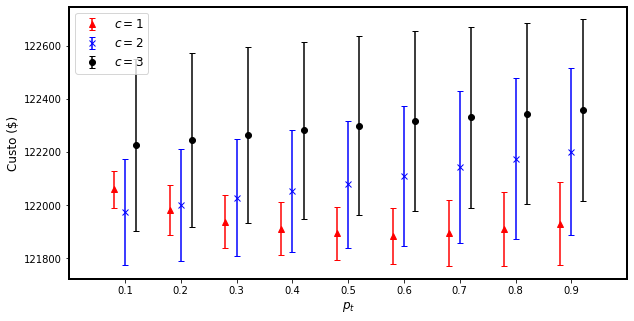
\includegraphics[width=120mm, height=60mm]{images/rgap2_40.png}

\fonte{Autor.}
\end{figure}

\begin{figure}[h]
    \caption{\label{rgap3_40}Configurações de $c$ e $p_t$ para $r^{gap}=3$ (caso 3).}
    \centering
    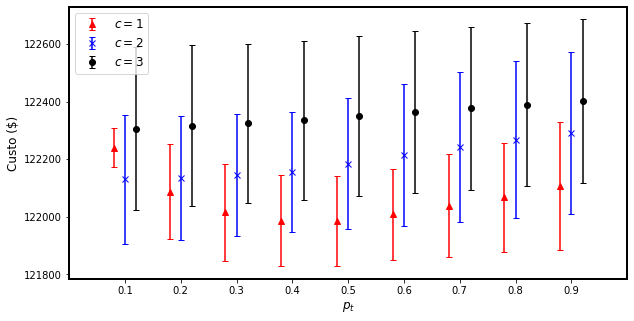
\includegraphics[width=120mm, height=60mm]{images/rgap3_40.png}
    \fonte{Autor.}
\end{figure}

\end{apendicesenv}
% ---

% ----------------------------------------------------------
% Anexos
% ----------------------------------------------------------

% ---
% Inicia os anexos
% ---
\begin{anexosenv}

% Imprime uma página indicando o início dos anexos
\partanexos

% ---
\chapter{Morbi ultrices rutrum lorem.}
% ---
\lipsum[30]

% ---
\chapter{Cras non urna sed feugiat cum sociis natoque penatibus et magnis dis
parturient montes nascetur ridiculus mus}
% ---

\lipsum[31]

% ---
\chapter{Fusce facilisis lacinia dui}
% ---

\lipsum[32]

\end{anexosenv}

%---------------------------------------------------------------------
% INDICE REMISSIVO
%---------------------------------------------------------------------
\phantompart
\printindex
%---------------------------------------------------------------------
% termina a cor

\end{document}
